\documentclass[toc=bibliographynumbered, liststotoc]{scrartcl} %mit [draft] vor den {} erreicht man, daß statt der Grafiken nur ein Rahmen in Größe der Grafik gezeichnet wird. Zusätzlich wird der Name der einzufügenden Datei in diesen Rahmen geschrieben]{book}
\usepackage[utf8]{inputenc}
\usepackage[T1]{fontenc}
\usepackage{lmodern}
%\usepackage[english,ngerman]{babel} %Deutsch als Hauptsprache, z.b. für Inhaltsverzeichnis etc.
\usepackage[ngerman,english]{babel} % Englisch als Hauptsprache!!!

\usepackage{graphicx}
\usepackage{xspace}
\usepackage{amstext}
\usepackage{amssymb}
\usepackage{setspace}
\doublespacing
\usepackage{longtable}
\usepackage{booktabs}
\usepackage{todonotes}
\usepackage{placeins}

\usepackage[paper=a4paper,margin=2.5cm]{geometry}
\usepackage{helvet}
\renewcommand*{\familydefault}{\sfdefault} %gehört zum Font


\usepackage{here} %erzwingt Platzierung von Bildern ("H" bei Option)
\usepackage{colortbl} % Tabellen: Spalten, Zeilen oder einzelne Zellen einfärben
\usepackage[round]{natbib}	%\citep   \cite
\bibliographystyle{apalike} % beides für Literaturverzeichnis bzw. Zitate

\usepackage{subfig} %lässt einen 2 Bilder oder Tabellen nebeneinander einfügen, mit dem Befehl "\subfloat[Unter-/Überschrift]{...}"
%\usepackage{subcaption}
\usepackage{rotating} %erlaubt das Drehen von Grafiken um 90° ohne angle=90
\usepackage{sidecap} %für Tabellen und Grafiken, die weiter sind als Textweite


% zum besseren Steuern des Anhangs /appendices statt /appendix benutzen

\usepackage[title,titletoc]{appendix}
\usepackage{lscape}


\newcommand{\bigcell}[2]{\begin{tabular}{@{}#1@{}}#2\end{tabular}}


\begin{document}

\begin{titlepage}
%\begin{figure}[t]
\begin{center}

\includegraphics[scale=0.65]{pics/hulogo.pdf}\\[1cm]

%\end{figure}
\textsc{\textbf{\normalsize LEBENSWISSENSCHAFTLICHE FAKULTÄT\\[0.2cm]  INSTITUT FÜR BIOLOGIE\\[1.5cm]
\LARGE MASTERARBEIT\\[0.5cm]
\normalsize ZUM ERWERB DES AKADEMISCHEN GRADES\\[0.5cm] MASTER OF SCIENCE\\[2cm]}
\normalfont %Kapitälchen deaktivieren
\textit{\large "Körpergrößentrends in fossilen Landschildkröten aus dem Neogen"\\[0.5cm]
"Body size trends in Neogene testudinid tortoises" }\\[2cm]
\small vorgelegt von\\[0.5cm] Julia Joos \\[0.2cm] geb. am 18.05.1991 in Freudenstadt \\[1cm] angefertigt in der Arbeitsgruppe Paläozoologie\\[0.2cm]
am Institut für Biologie/Museum für Naturkunde\\[1cm]
Berlin, im Septenber 2017}
\end{center}


\end{titlepage}


\tableofcontents
\newpage
\listoffigures  
\newpage                       
\listoftables                     
\newpage
\section{Introduction}
\subsection{Body size evolution}

%Laurin, 2004
The body size of organisms has been of interest to researchers for a long time \citep{Haldane1928,Peters1983}. It is a universal trait, that can be easily measured and compared among different organisms \citep{.}. Furthermore, it is readily available for many animals in the fossil record which allows for comparison with extant species \citep{.}. A number of biotic and abiotic factors including habitat, resource availability, competition, climate and many more influence body size and it is linked to ecological and evolutionary processes \citep{Blackburn1994a,Blueweiss1978,Smith2009}.
%, for example \todo{example?!}.
Patterns of body size variation across spatial and/or temporal scales have been described for many animal groups and some have been summarised as ecological rules \citep{Millien2006,Angielczyk2015}.
%and many biogeographical rules concern body size evolution: 
Cope's rule describes the gradual within-lineage body size increase over time \citep{Cope1887}. According to the island rule large species become smaller on islands while small species often show an increase in body size \citep{Foster1964}. Bergmann's rule \citep{Bergmann1848} states that animals attain larger at higher latitudes, which can be considered a special case of the temperature-size rule, which predicts an increase in body size at lower temperatures \citep{AngillettaJr2004a}.
While such patterns have been well documented
%described in many animal groups and species 
\citep{Millien2006}, the underlying mechanisms might not be the same in all taxa and require further investigation \citep{Smith2009}.
The development of body size or any other trait over time can follow different evolutionary trajectories, that describe general trends of trait evolution. If a trait does not significantly change, it is described as stasis. If a trait does change, this change can either be directional, referred to as a generalized random walk, or non-directional, which is described as an unbiased random walk. Recently, new analytical tools have been developed, to be able to determine which evolutionary model fits the development of a trait, for example size trends, best over time \citep{Hunt2006,Hunt2015}.
Changes in body size on the clade level can either be due to selective forces acting on the whole clade (trends) or individual species being influenced by different causes (tendencies) \citep{Hunt2006}. A trend can be an increase or decrease in minimum, mean or maximum size and can be caused by differing speciation and extinction rates and therefore occur independently of tendencies \citep{Smith2016}. Maximum size, for example, is usually expected to increase without being selected for \citep{Smith2016}.

%Smith et al., 2016
%However, when patterns of size increase are examined within lower-level taxa (e.g., phyla, classes), the trends found there are generally more consistent with the null (Table 2)

%\todo{include evolutionary models here!!}


\subsection{Maximal body size - Megafauna}
Many taxa have a right-skewed body size distribution, which means that smaller body sizes are more abundant than large ones \citep{Blackburn1994a,Kozlowski2002,Lyons2008}. This raises the question of why organisms are a certain size, if there is an optimal body size for each organisms, why some species attain larger sizes than others and which 
structural, physical and physiological properties determine and limit minimum or maximum body size
%the maximum possible body size depends on, structurally, physically and physiologically 
\citep{Smith2009}.
%are distribution yA potential optimal body size and extreme body size - either large or small - are of particular interest to many researchers . 
A large body size is associated with certain advantages, e. g. decreased predation risk, higher fasting endurance, higher competitive ability, all of which results in a higher fitness \citep{.}.
On the other hand, there are some disadvantages to having a larger body size since usually a larger range size and more resources are needed and generation times are often longer \citep{.}.
%a lot of implications regarding resource availability, resilience, fecundity, 
%but it has also been debated whether larger body sizes may entail a higher risk of extinction (...).
In the history of Earth, animals have again and again attained very large body sizes, although patterns of when and how often maximum body size is achieved are inconsistent across time and different animal groups \citep{Smith2016}.
%(Also, different patterns in minimum size, which could be due to poorer preservation of smaller forms.)
Some famous examples of giant forms are the large insects from the Carboniferous/Permian period, the giant non-avian dinosaurs from the Jurassic/Triassic, the giant mammals from the Quatenary or today's largest animal, the blue whale \citep{.}.
%Giant animal forms are often intrigiung, because they usually present the upper limit of what is possibe physically, physiologically and structurally. 
%For example, the large insect (dragonflies etc.) from the Carbonian/Permian border (?) seem absolutely surreal to us as well as the later non-avian dinosaurs, which still fascinate many people. And today's largest animal, the blue whale, is of interest to many people.
Animals with a body mass exceeding 44 kg (or sometimes 10 kg \citep{Sandom2014}) are referred to as megafauna \citep{Barnosky2004, Rhodin2015}.
%Animals are considered megafauna, if their body mass/body length exceeds 44 kg \citep{Barnosky2004} .
%Large size can have many advantages but also some disadvantages.
%Especially the mammalian megafauna has been in the focus of research, wooly mammoths, giant sloths, waldelefanten?, etc.
It has been suggested, that large animals are more prone to extinction than smaller ones \citep{.}. Reasons for this may be that large species usually need more resources, have a larger range and longer generation times \citep{.}. 
During the Quaternary, a huge number of large mammals which were considered megafauna went extinct \citep{.}.
A number of causes for these extinction events have been discussed, but while a meteorite and disease were dismissed as possible causes due to lack of evidence \citep{.}, two possible scenarios are still under discussion: climate change and anthropogenic influence \citep{.}.
Some recent studies suggest that human influence has been the main driver of these extinctions of mammalian megafauna \citep{Barnosky2004,Sandom2014,Gibbons2004,Schuster2000}.

%- extinctions seem to be more size-biased in vertebrates

While the mammalian megafauna as well as their extinction %Pleistocene extinctions 
have been well investigated, the herpetofauna has also lost a considerable number of species during the Quaternary \citep{Blain2016}. 
For example, many turtle and tortoise species have gone extinct, among those quite a few large species \cite{Rhodin2015}.
In former times, giant tortoises were abundant on the continents as well as on many islands, whereas today giant tortoises are present only on two island regions in the tropics \citep{.}
% - the Galapagos islands and the West Indian islands
.


%Some basic questions deal with the issue of optimal body size: is there one for every organism and if so, how is it determined, how does it evolve?
%Animals --> magintudes of body size, many have their greatest body size right now, possible maximum has not been reached! BUT reptiles not


% Smith et al., 2016:
%For body size evolution in particular, the most commonly observed and documentable kind of trend—a rise in the maximum—does not by itself tell us much about underlying tendencies. Maxima are expected to increase even if no tendencies, no evolutionary forces, are present. Thus, we cannot infer the existence of a selective advantage of large size merely from an increase in the maximum.
%If a clade first evolves at a size close to the minimum size possible for a particular body plan or ecology and subsequent speciation events are random with respect to size (i.e., descendants are equally likely to be larger or smaller than their ancestors), thenmean size will increase, because the lower bound prevents the variance from increasing in the direction of smaller sizes. This is an example of a passive trend, one with no increasing tendency.
%A positive association between body size and extinction risk has been demonstrated for Pleistocene and living mammals (Lyons et al. 2004, Davidson et al. 2009), marine and fresh- water fishes (Olden et al. 2007), and birds (Boyer 2010). The association between body size and extinction risk is widely interpreted to result from the inverse association of body size with ecologically important traits such as population size, fecundity, and total resource requirements (Brown 1995).



%\subsection{Megfauna extinctions (mammals)}


%\subsection{Ectothermic megfauna}

%--> dinos BUT also giant tortoises


\subsection{Giant Tortoises - Testudinidae}
In the fossil record two clades of terrestrial tortoises have been identified, which both contained giant forms. One is the family Meiolaniidae, which occurred exclusively in Australia and is completely extinct nowadays \citep{.}. The other is the family Testudinidae, which comprises all extant terrestrial tortoises as well as many extinct or fossil taxa \citep{.}. The testudinids included giant forms and occurred on all continents but Australia \citep{.}.
Testudinidae have been known in the fossil record from the Eocene on, the earliest fossils stemming from Africa \citep{.}.
Body size played an important role in the earlier times of testudinid taxonomy \citep{.}. In the beginning, all tortoise fossils were assigned to the genus Testudo, but around the 20th century(??), tortoises were grouped into two clades based on body size. Large taxa were all assigned to the genus \textit{Geochelone}, while small tortoises were assigned to \textit{Testudo}.
Eventually, over the past few decades, the taxonomy has been revised for many regions, based on morphological and biogeographical clues \citep{.}. In the Americas, all tortoises are now referred to as either \textit{Hesperotestudo}, \textit{Gopherus} or \textit{Chelonoidis}, the latter contains all extant Galapagos giant tortoises \citep{.}. In Europe, the genus \textit{Cheirogaster} has been introduced but is currently being replaced by \textit{Titanochelon}, although not all species have been revised accordingly yet \citep{.}. Small species still belong to \textit{Testudo}, which contains the extant \textit{Testudo graeca}-group \citep{.}.
In Asia and Africa, the two current biodiversity hotspots for turtles and tortoises in general \citep{.}, many different taxa have now been differentiated \citep{.}.
In Asia, the genera \textit{Geochelone}, \textit{Indotestudo} and \textit{Manouria} are present \citep{.}. On mainland Africa there are seven extant genera: \textit{Homopus}, \textit{Psammobates}, \textit{Kinixys}, \textit{Malacochersus}, \textit{Chersina}, \textit{Stigmochelys} and \textit{Centrochelys}, the latter consisting of one species, \textit{Centrochelys sulcata}, which is the largest extant continental tortoise with a carapace length of about 80 cm \citep{.}. In the West Indian Islands (Madagascar, Seychelles, Aldabra etc.), there are three extant gerena, \textit{Astrochelys}, \textit{Pyxis} and the giant \textit{Aldabrachelys}, as well as the extinct \textit{Cylindraspis} \citep{.}.

On the contintents as well as remote islands giant tortoises exceeding carapace lengths of 2 m were abundant in former times and have frequently been found in fossil deposits \citep{.}. The presence of large tortoises on islands has been explained by their ability to float and to survive for months without water or food \citep{Gerlach2006, Patterson1973, Cheke2016}. 
%Cheke et al. 2016: Meilania also floated to islands!!

%The colonization of islands has been achieved by tortoises due to their resilience, they can cope without food or water for months (which is why they have been exploited by humans in the past --> whaling industry), their bouyancy. 

However, the abundance of giant tortoises on these remote oceanic islands along with their resilience and survivability without resources made them a very attractive food item for humans, especially in the whaling industry \citep{.}.
In addition to the exploitation of giant tortoises on islands, both small and large tortoises and turtles were also frequently eaten on the mainland \citep{.}.
%But also on the mainlands, and also small species have frequently been eaten, since turtles and tortoises 
Tortoises are easily captured, do not need a great amount of preparation before they can be cooked and can even be kept as a "staple" since they stay alive for quite a while withoud food or water \citep{Thompson2002,Thompson2014}. Intensive hunting and exploitation has been suggested to affect tortoise body size \citep{.} since larger individuals are more easily visible and yield more meat, they are more prone to exploitation than small ones \citep{Rhodin2015}. This may have lead to a decreased body size within a tortoise population, where tortoise consumption is common.
For this reason, tortoise body size has even been suggested as a proxy for human population size in some areas \citep{Steele2005,Stiner1999,Stiner2000}.
To this day, turtles and tortoises are still being eaten in some countries, although many are endangered \citep{.}.
Apart from anthropogenic influences, climate probably also affected tortoises \citep{.}. 
As ectotherms, turtles and tortoises are inherently more dependent on climate than endotherms \citep{.}. Especially large tortoises are very temperature-sensitive due to their unique physiology and morphology \citep{Swingland1979a, Swingland1979b}. In the fossil record, large tortoises are considered to be an indicator for mild winters in \citep{Hibbard1960,Schleich1981}, since they are thought to not have been able to dig themselves burrow for hibernation like modern Gopherus tortoises do (?? only in some places, I guess?)\citep{Carlson1999, Stojanov2009}. Additionally, giant tortoises run a high risk of overheating and display behavioral thermoregulation to keep their body temperature below a dangerous or even lethal value \citep{Sturbaum1982, Schleich1981}.
It has not been concluded with certainty, if anthropogenic influence or climate change or a mixture of both have caused the extinction of giant tortoises\citep{.}.

% \todo{over which time period??} 

%There, giant tortoises were abundant, just like they have been until a couple of hundreds of years ago on the Galapagos islands. On the West Indies, 2 species of Aldabrachelys actually went extinct in the past centuries (??)
 
%- mention Meiolania?
%- taxonomy
%- occurence
%- evolution/distribution
%- tortoises are temperature sensitive (?), well, giant tortoises seem to be.
%- have always been a preferred food source for humans (whaling industry)

\subsection{Body size trends in Testudinidae}

The aim of this work is to identify general body size distributions in tortoises (Testudinidae) on a global scale across the last 20 million years. Further, to investigate the general evolutionary mode of body size in testudinidae. 
%For this, the methods of Hunt (...) are used, which fit the mean trait, in this case carapace length, over time to different evolutionary models: either stasis, unbiased random walk or a generalized random walk. ... These mean and have been tested for ....????
Apart from that, focusing on giant tortoises, which were abundant in former times, but are extinct nowadays apart from a few remaining populations on tropical islands, to discuss where and when they occurred in the fossil record and which underlying reasons for the extinction of many giant forms have been stated in the literature.
Understanding how and why giant tortoises went extinct in the past, can hold valuable information for conservation work today. Many tortoise species are endangered and extinction rates have been especially high for insular species since the Pleistocene \citep{Rhodin2015}.

%- general body size distribution on a temporal and spatial scale
%- when/where did giant tortoises occurr, when/where did they disappear?
%- evolutionary mode of giant tortoises
%- how did they go extinct?


%- unbiased random walk: descendants are equally likely to be larger or smaller than their ancestors

\newpage
\section{Material \& Methods}

\subsection{Data collection}
I collected data on body size of fossil testudinids from the Upper Miocene until recent times. The body size data set includes 26 genera, comprising over 70 fossil and extant species. The majority of the data was obtained from the primary literature (\ref{TabS1}). To find relevant publications, I relied mostly on the references listed in FosFarBase (CITE), PDBD (cite), and "Fossil Turtle Checklist (CITE).
Furthermore, the FosFarBase provided fossil occurences of testudinids all over the world, including their exact localities and age (\ref{TabS2}), which were used to get an overview over the availability of body size data. 
For extant taxa, I measured dry material (n = 67) from the collection of the Museum für Naturkunde zu Berlin (MFN). In addition, body size data from the literature was included (\ref{TabS3}).

\subsection{Body size estimation}
Body size is reported as straight carapace length (SCL). Where SCL was not available from the primary literature, it was estimated either from plastron length (PL), femur length or humerus length (\ref{TabS1}). For carapace length estimations based on plastron length, the measurements from the MFN collection material was used to calculate the ratio between SCL and PL. Since the SC/PL ratio was similar for all species and genera, a single general ratio was calculated for all testudinids and hence used for the SCL estimations unless stated otherwise. For estimations based on humeri or femora, the ratios provided by Franz et al. (2001) were used.

TO DO: check Franz \& Quitmyer, 2005 again!! (CL regression)

\subsection{Analyses}
All subsequent analyses were performed with R (version ...), including the packages dplyr (cite) to manipulate the data and ggplot2 (cite) to create figures. Species Accumulation Curves were created to see if sample size sufficed. This was repeated on genus level, since genera of fossil testudinids are relatively well resolved by now whereas determination on the species level is still somewhat obscure in many cases, as quite some species were based on scarce material. Since the data set relies on literature, occurrences increase with each added reference and reach a maximum, when no new species/genera are added.



- only used samples > 11.000 mya?!

\subsection{Body size trends over time}
To investigate trends in body size over time, the R package paleoTS (cite) was used. Data were split into time bins according to the stratigraphic timescale (\ref{Tab1}). 
\newpage
\section{Results}

%read Willis et al., 2010 and Willis and Fortey, 2003 on use of paleontological data.

% read Thompson and Withers, 2003: Species Accumulation Curve
\subsection{Sample-based accumulation curves}
The sample-based accumulation curve (SAC) on the generic level shows a relatively low intial slope and a long upward slope to the asymptote, which does not reach full saturation (Fig. \ref{fig:SACGen}).
%Although the SAC does not completely plateau, considering the large area covered and the high number of rare genera in the dataset, it can be considered well enough sampled for our purposes.
In contrast, the species accumulation curves, both per reference and per locality, show only a slight initial increase and, for the same number of references/sampling units, are far from reaching an asymptote (Fig. \ref{fig:SACall} (a), (b)).
% DISCUSSION: as could be expected, since there are less genera than species \citep{Gotelli2001}. At a large geographic scale, it can be expected, that an asymptote is not reached \citep{Thompson2002}. Fig. \ref{fig:SACGen} corresponds to the shape one would expect, when there are many genera that are rare and only a few abundant ones. For the different continents, only Europe and Eurasia show some sort of "typical" SAC shape.
%%%____
% DISCUSSION ? 
%Since there are less genera than species, it is to be expected that genera reach an asymptote earlier than species.
%%%____
Accumulation curves for individual continents show that Europe reflects the trend of the overall dataset, with a long upward slope after the inflection point, whereas the other continents require further sampling (Fig. \ref{fig:SACall} (c) - (i)). For this reason, the timescale analysis was only conducted for Europe and Eurasia, but not for the other continents.

%--> genera sufficiently sampled, species not
%--> for genera, when splitting up continents only Europe and Eurasia are sampled well enough --> ask Johannes again, I feel like Asia is screwing up the results, would stick with Europe.
%--> maybe refer to table 20: overview over fossil genera per time bin??

%_______________________________________________________________________
\begin{figure}[htbp]
	\centering
	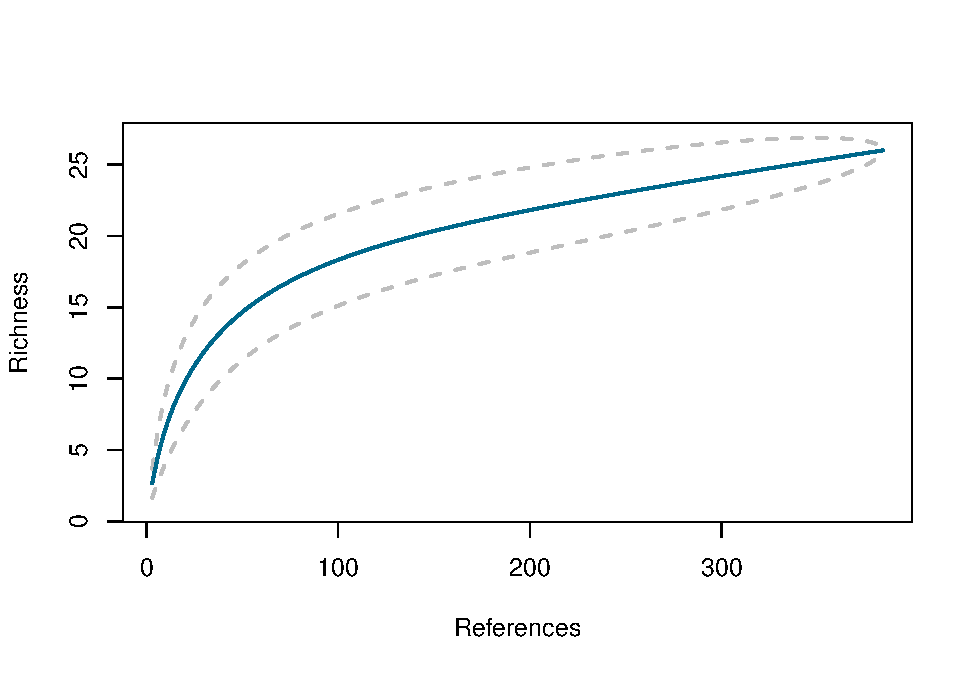
\includegraphics[width=0.8\textwidth]{MA_JJ_files/figure-latex/SACGenera-1.pdf}
	\caption[Sample-based accumulation curve on generic level]{Sample-based accumulation curve of fossil genera per reference. Dashed lines represent the confidence inteval.}
	\label{fig:SACGen}
\end{figure}


\FloatBarrier


%read: Smith and Lyons, 2010 (?) and Smith et al., 2016
%--> body size patterns (see also table 22, general statistics)

%data is bimodal (not normally distributed --> fig. ), still visible in pretty much all subgroups that you could split them into.
%as most animal groups/clades (?) right-skewed = smaller body size more frequent, BUT island species are left-skewed with more larger body sizes! (logtransformed data, skewness: negative for Zanclean, Messinian ??, insular, fossil-insular, but not modern-insular!!)
\subsection{Descriptive statistics}

The histograms indicate that testudinid body size is not normally distributed (Fig. \ref{fig:histAll}), which is supported by QQ-Plots for raw as well as log-transformed data (Fig. \ref{fig:NormDis}).

The body size distribution is moderately right-skewed (Table \ref{tab:stats}), with a higher frequency of smaller body sizes.
Body size ranges from a minimum of 80 mm to a maximum of 2500 mm for the entire data set. When comparing body sizes on a temporal scale, the minimum body size per stratigraphic stages excluding modern taxa ranges from 90 mm to 270 mm, while the maximum 1100 mm to 2500 mm. The highest maximum body size was observed in the fossil record from continental Europe (CL = 2500 mm).
%________________________________________________________________________

\begin{figure}[htbp]
	\centering
	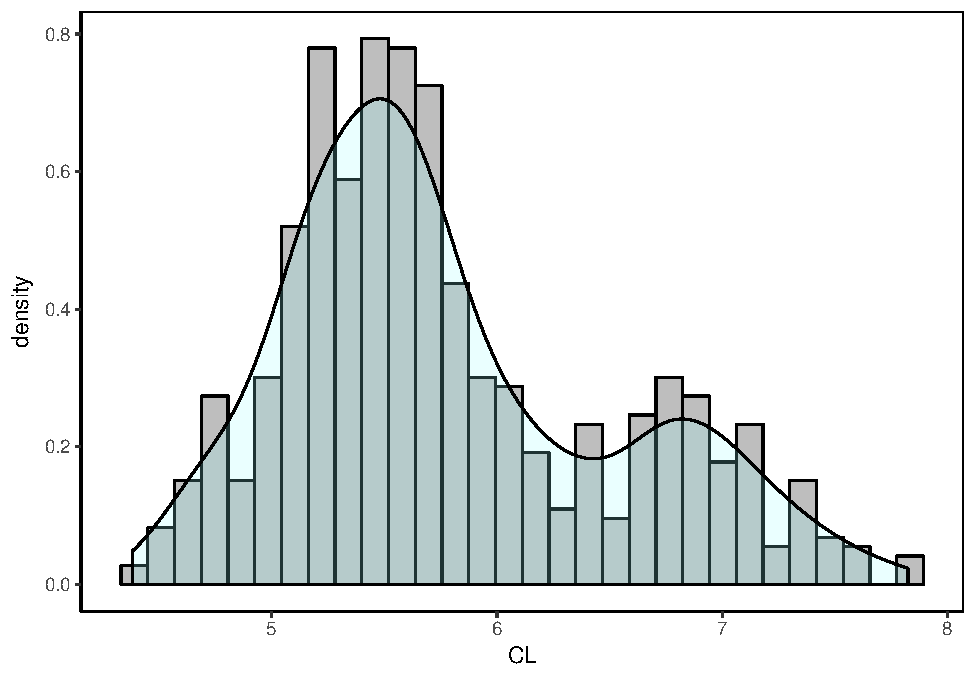
\includegraphics[width=0.8\textwidth]{MA_JJ_files/figure-latex/HistAll-1.pdf}
	\caption[CL distribution]{Body size distribution of complete data set. Bimodally distributed and right-skewed.}
	\label{fig:histAll}
\end{figure}

This pattern is also apparent when splitting the data set into fossil and modern taxa (Fig. \ref{fig:HistFMCI} (a)). Considering insularity, body size distribution is right-skewed for continental taxa, but left-skewed for insular species, meaning larger body size is more frequent than smaller body size on islands. Insular taxa are also left-skewed when only considering fossil taxa, but modern insular taxa have a skewness close to 0, indicating a symmetric distribution (Table \ref{tab:stats}).
Kurtosis suggests light tails with no/few outliers (kurtosis < 3) for insular and modern insular species, whereas continental species have a heavy tail (kurtosis > 3; Table \ref{tab:stats}).

\begin{center}
	\begin{figure}[htbp]
		\subfloat[Fossil vs. modern]{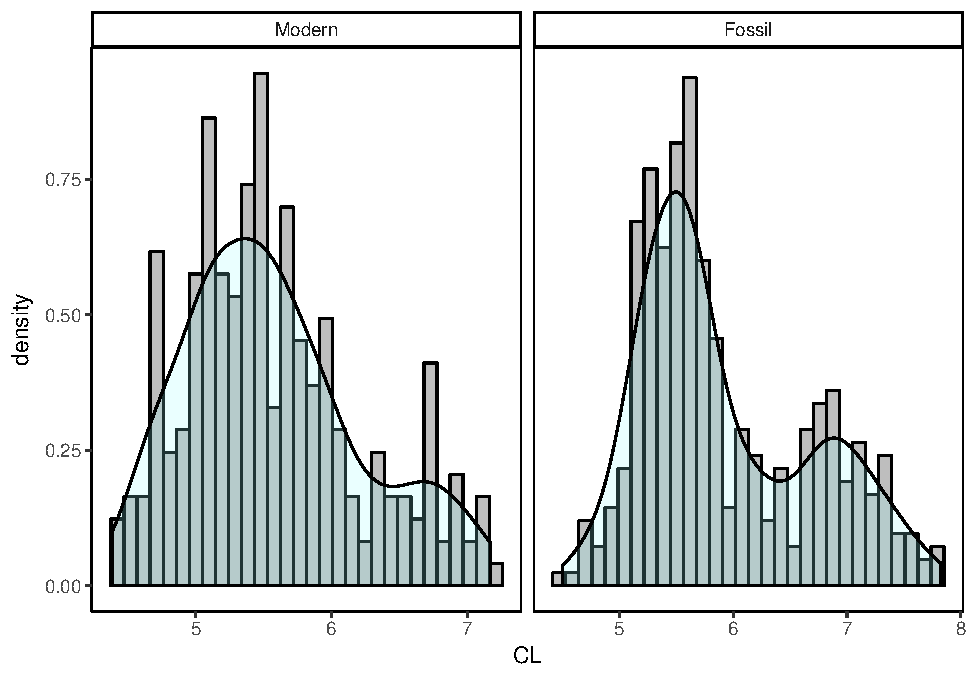
\includegraphics[scale=0.45]{MA_JJ_files/figure-latex/HistFosMo-1.pdf}}
		\subfloat[Continental vs. insular]{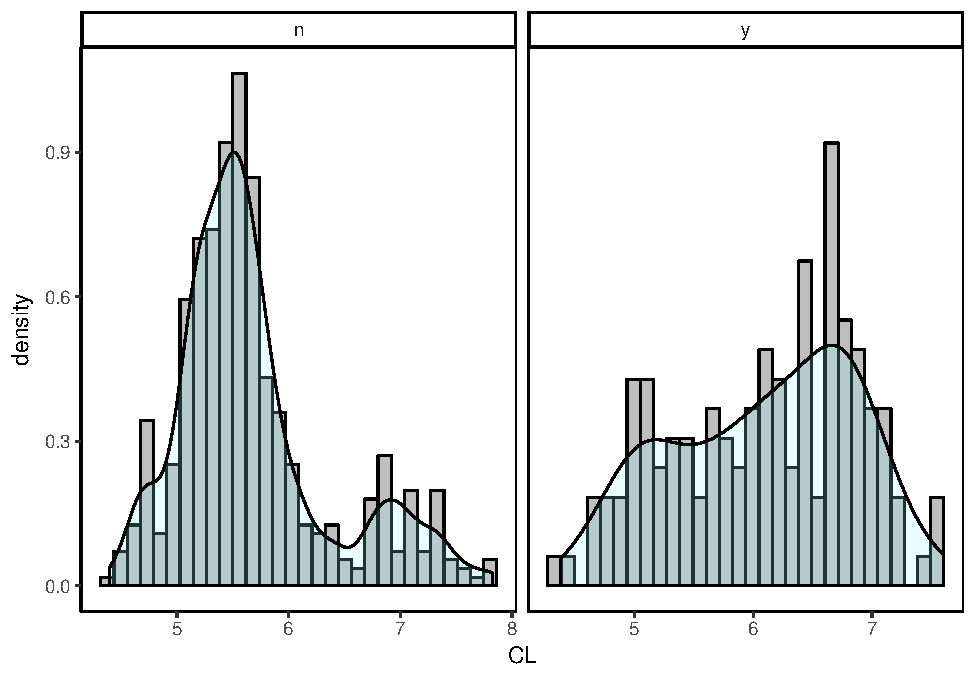
\includegraphics[scale=0.45]{MA_JJ_files/figure-latex/HistCI-1.pdf}}	
		\caption[Fossil vs. modern, continental vs. insular.]{Histograms for fossil vs. modern and continental vs. insular data.}
		\label{fig:HistFMCI}
	\end{figure}
\end{center}

The histograms show a bimodal distribution, wich is also apparent on most sublevels, except for modern insular species (Fig. \ref{fig:HistRest} (a)).
Body size distributions are similar, right-skewed and bimodal, for the four continents and reflect the overall trend (Fig. \ref{fig:HistRest} (b)).




\FloatBarrier

%__________________________



Mean body size differs significantly across time bins (Kruskal Wallis Test, $\chi^2$ = 71.441, P < 0.01; Fig. \ref{fig:boxBins}). 
The multiple comparison test showed that modern median body size is smaller than body size in the Upper Pleistocene. %(Wilcoxon Rank Sum Test, W = 3853.5, P < 0.01 )
There is no difference in body size within the Pleistocene %(Wilcoxon Rank Sum Test, P > 0.05)
and Pleistocene body size does not differ from body size in the Upper Miocene%(Wilcoxon Rank Sum Test, P > 0.05)
. Serravallian body size is smaller than Langhian body size in the Middle Miocene%(Wilcoxon Rank Sum Test, W = 45, P < 0.01)
, but Langhian body size is not different from Lower Miocene body size%(Wilcoxon Rank Sum Test, W = 311, P = 0.06)
.


%__________________________________________________________________________
\begin{figure}[hbtp]
	\centering
	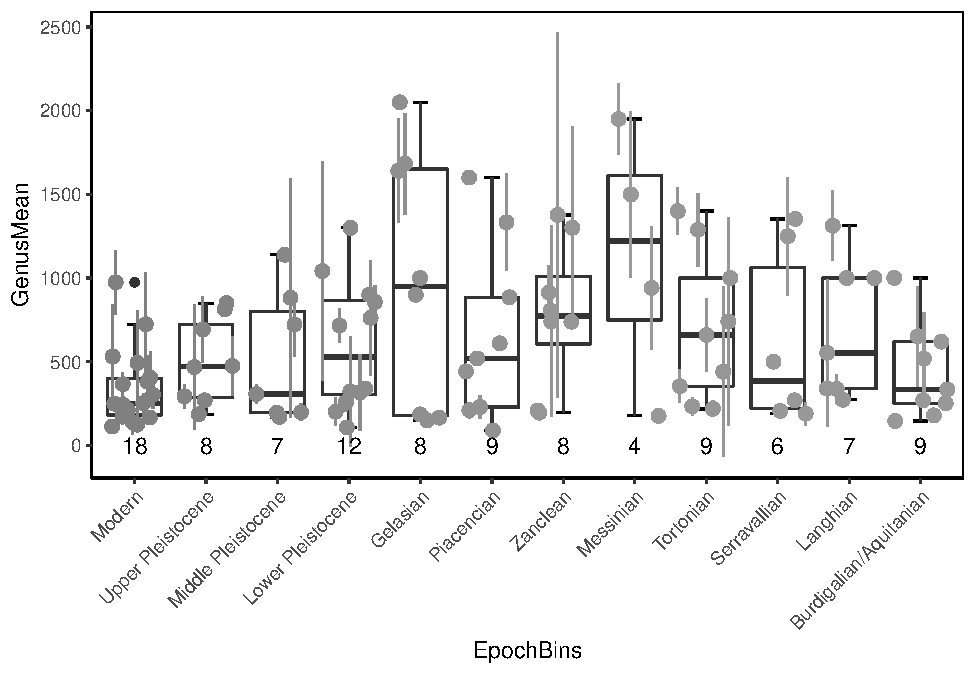
\includegraphics{MA_JJ_files/figure-latex/BPGBins-1.pdf}
	\caption{Boxplots of mean CL per time bin, including mean and sd CL for
		each genus (as pointrange).}
	\label{fig:boxBins}
\end{figure}

%\todo{random sampling necessary?}
% = 71.441, df = 11, p-value = 6.496e-11


%need statistics for boxplot!! kruskal-wallis-test plus post-hoc test (+ bonferroni correction?) or moving mean (faysal?)
%you can kind of see how the median increases and then decreases again
%(compare in order: Modern < Upper Pleistocene etc., do median and variance??)

% FOR ALL TIME STAGES

%	Kruskal-Wallis rank sum test

%data:  list(M, UPle, MPle, LPle, G, Pia, Z, Mess, Tort, S, L, BA)
%Kruskal-Wallis chi-squared = 71.441, df = 11, p-value = 6.496e-11

%Multiple comparison test after Kruskal-Wallis 
%p.value: 0.05 
%Comparisons
%obs.dif critical.dif difference
%Modern-Upper Pleistocene                  116.987013     93.54915       TRUE
%Modern-Middle Pleistocene                  80.140652     90.54349      FALSE
%Modern-Lower Pleistocene                   66.123604     87.87753      FALSE
%Modern-Gelasian                             1.627566    114.05459      FALSE
%Modern-Piacencian                         113.296537    136.11314      FALSE
%Modern-Zanclean                           205.945804    123.43828       TRUE
%Modern-Messinian                          137.122727    193.24680      FALSE
%Modern-Tortonian                           61.739394     96.96976      FALSE
%Modern-Serravallian                        21.764310    121.34770      FALSE
%Modern-Langhian                           202.487013    164.56067       TRUE
%Modern-Burdigalian/Aquitanian              70.472727    115.73561      FALSE
%Upper Pleistocene-Middle Pleistocene       36.846361    118.78423      FALSE
%Upper Pleistocene-Lower Pleistocene        50.863409    116.76486      FALSE
%Upper Pleistocene-Gelasian                115.359447    137.55006      FALSE
%Upper Pleistocene-Piacencian                3.690476    156.32773      FALSE
%Upper Pleistocene-Zanclean                 88.958791    145.42551      FALSE
%Upper Pleistocene-Messinian                20.135714    207.98052      FALSE
%Upper Pleistocene-Tortonian                55.247619    123.75260      FALSE
%Upper Pleistocene-Serravallian            138.751323    143.65527      FALSE
%Upper Pleistocene-Langhian                 85.500000    181.63641      FALSE
%Upper Pleistocene-Burdigalian/Aquitanian   46.514286    138.94713      FALSE
%Middle Pleistocene-Lower Pleistocene       14.017047    114.37094      FALSE
%Middle Pleistocene-Gelasian                78.513086    135.52379      FALSE
%Middle Pleistocene-Piacencian              33.155885    154.54785      FALSE
%Middle Pleistocene-Zanclean               125.805152    143.51048      FALSE
%Middle Pleistocene-Messinian               56.982075    206.64601      FALSE
%Middle Pleistocene-Tortonian               18.401258    121.49644      FALSE
%Middle Pleistocene-Serravallian           101.904962    141.71632      FALSE
%Middle Pleistocene-Langhian               122.346361    180.10681      FALSE
%Middle Pleistocene-Burdigalian/Aquitanian   9.667925    136.94153      FALSE
%Lower Pleistocene-Gelasian                 64.496038    133.75738      FALSE
%Lower Pleistocene-Piacencian               47.172932    153.00123      FALSE
%Lower Pleistocene-Zanclean                139.822200    141.84356      FALSE
%Lower Pleistocene-Messinian                70.999123    205.49188      FALSE
%Lower Pleistocene-Tortonian                 4.384211    119.52289      FALSE
%Lower Pleistocene-Serravallian             87.887914    140.02804      FALSE
%Lower Pleistocene-Langhian                136.363409    178.78144      FALSE
%Lower Pleistocene-Burdigalian/Aquitanian    4.349123    135.19364      FALSE
%Gelasian-Piacencian                       111.668971    169.39706      FALSE
%Gelasian-Zanclean                         204.318238    159.39129       TRUE
%Gelasian-Messinian                        135.495161    217.97454      FALSE
%Gelasian-Tortonian                         60.111828    139.89893      FALSE
%Gelasian-Serravallian                      23.391876    157.77782      FALSE
%Gelasian-Langhian                         200.859447    192.99946       TRUE
%Gelasian-Burdigalian/Aquitanian            68.845161    153.50345      FALSE
%Piacencian-Zanclean                        92.649267    175.85199      FALSE
%Piacencian-Messinian                       23.826190    230.28513      FALSE
%Piacencian-Tortonian                       51.557143    158.39839      FALSE
%Piacencian-Serravallian                   135.060847    174.39088      FALSE
%Piacencian-Langhian                        89.190476    206.80215      FALSE
%Piacencian-Burdigalian/Aquitanian          42.823810    170.53342      FALSE
%Zanclean-Messinian                         68.823077    223.02794      FALSE
%Zanclean-Tortonian                        144.206410    147.64914      FALSE
%Zanclean-Serravallian                     227.710114    164.68880       TRUE
%Zanclean-Langhian                           3.458791    198.68908      FALSE
%Zanclean-Burdigalian/Aquitanian           135.473077    160.59847      FALSE
%Messinian-Tortonian                        75.383333    209.54137      FALSE
%Messinian-Serravallian                    158.887037    221.87771      FALSE
%Messinian-Langhian                         65.364286    248.16258      FALSE
%Messinian-Burdigalian/Aquitanian           66.650000    218.85882      FALSE
%Tortonian-Serravallian                     83.503704    145.90588      FALSE
%Tortonian-Langhian                        140.747619    183.42158      FALSE
%Tortonian-Burdigalian/Aquitanian            8.733333    141.27276      FALSE
%Serravallian-Langhian                     224.251323    197.39708       TRUE
%Serravallian-Burdigalian/Aquitanian        92.237037    158.99725      FALSE
%Langhian-Burdigalian/Aquitanian           132.014286    193.99761      FALSE


% FOR MODERN - PLEISTOCENE - PLIOCENE - MIOCENE
%Kruskal-Wallis rank sum test

%data:  list(Modern, Plei, Plio, Mio)
%Kruskal-Wallis chi-squared = 37.764, df = 3, p-value = 3.172e-08


%Multiple comparison test after Kruskal-Wallis 
%p.value: 0.05 
%Comparisons
%obs.dif critical.dif difference
%Modern-Pleistocene   110.904114     49.80480       TRUE
%Modern-Pliocene       67.623302     58.35513       TRUE
%Modern-Miocene        64.510137     49.57182       TRUE
%Pleistocene-Pliocene  43.280812     64.36704      FALSE
%Pleistocene-Miocene   46.393977     56.52575      FALSE
%Pliocene-Miocene       3.113165     64.18694      FALSE



%__________________________________________________________________________
\begin{center}
	\begin{figure}[htbp]
		\subfloat[Fossil vs. modern]{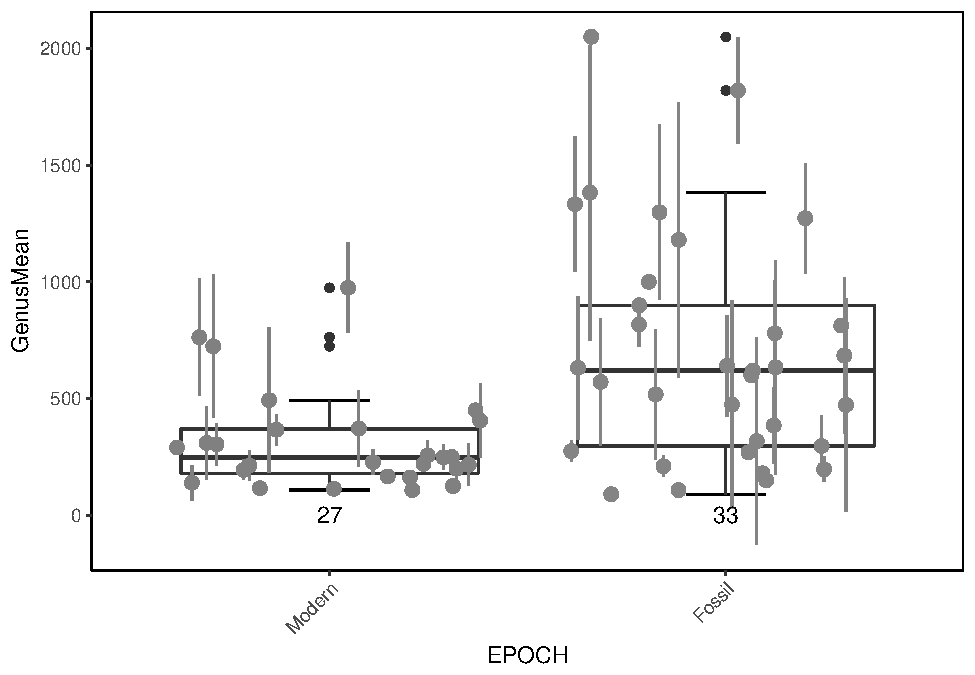
\includegraphics[scale=0.45]{MA_JJ_files/figure-latex/BPMF-1.pdf}}
		\subfloat[Continental vs. insular]{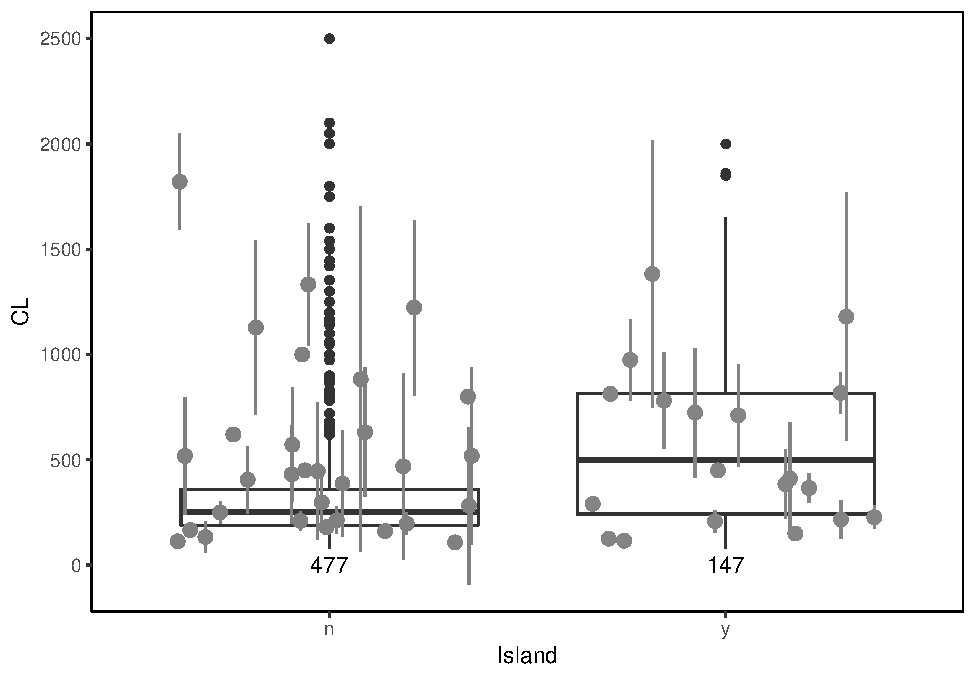
\includegraphics[scale=0.45]{MA_JJ_files/figure-latex/BPCI-1.pdf}}
		\caption{Boxplots of CL split into fossil vs. modern (a) and cotinental vs. insular (b)}
		\label{fig:boxFMCI}
	\end{figure}
\end{center}



Comparison of modern and fossil testudinids showed that modern tortoises are significantly smaller than fossil ones (Wilcoxon Rank Sum Test, W = 22318, P < 0.01; Fig. \ref{fig:boxFMCI}). Furthermore, continental testudinids are significantly smaller than insular taxa (Wilcoxon Rank Sum Test, W = 13854, P < 0.01; Fig. \ref{fig:boxFMCI}).
These results can even be considered in combination: modern continental taxa are smaller than fossil continental taxa (Wilcoxon Rank Sum Test, W = 8046, P < 0.01; Fig. \ref{BoxFoMCI}) and modern insular taxa are smaller than fossil insular taxa (Wilcoxon Rank Sum Test, W = 631.5, P < 0.01; Fig. \ref{BoxFoMCI}))

Finally, body size differs among continents (Kruskal Wallis Test, $\chi^2$ = 34.343, P < 0.01; Fig. \ref{fig:boxCon}). The multiple comparison test showed that African testudinids differ significantly from the other three continents in body size. American testudinid body size is comparable to that of Asia, but differs from those of Africa and Europe. Furthermore, Asian and European testidinids are similar in body size. %Since only Europe/Eurasia are well sampled, these relationships could change with further sampling. ??


\begin{figure}[htbp]
	\centering
	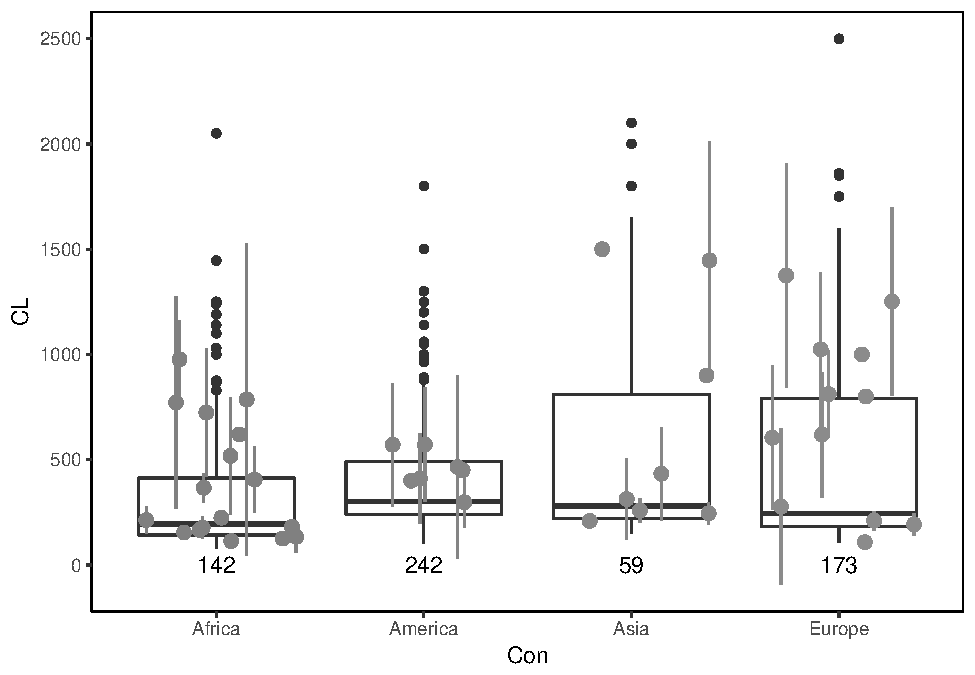
\includegraphics[width=0.75\textwidth]{MA_JJ_files/figure-latex/BPCon-1.pdf}
	\caption{Boxplot: body size on different continents, genera summarised}
	\label{fig:boxCon}
\end{figure}



\FloatBarrier
%__________________________________________________________________________

\subsection{paleoTS analysis}\label{paleots-analysis}




\subsubsection{complete dataset}\label{all-continental-and-insular}

Fitting of the three evolutionary models favoured stasis for the entire data set, although model support was only 51\,\% followed by 33\,\% support for the unbiased random walk (Fig. \ref{fig:pTSall}, Table \ref{tab:pTSall}). When solely considering continental genera, the best-fitting model was the unbiased random walk, but again not ideally supported with 55\,\% followed by a modest model support of 30\,\% for generalized random walk (Fig. \ref{fig:pTSC}, Table \ref{tab:pTSCEM}). In contrast, insular genera are best described by stasis, which was very well supported (100\,\%; Fig. \ref{fig:pTSI}, Table \ref{tab:pTSIEM})). 


\begin{figure}[H]
	\centering
	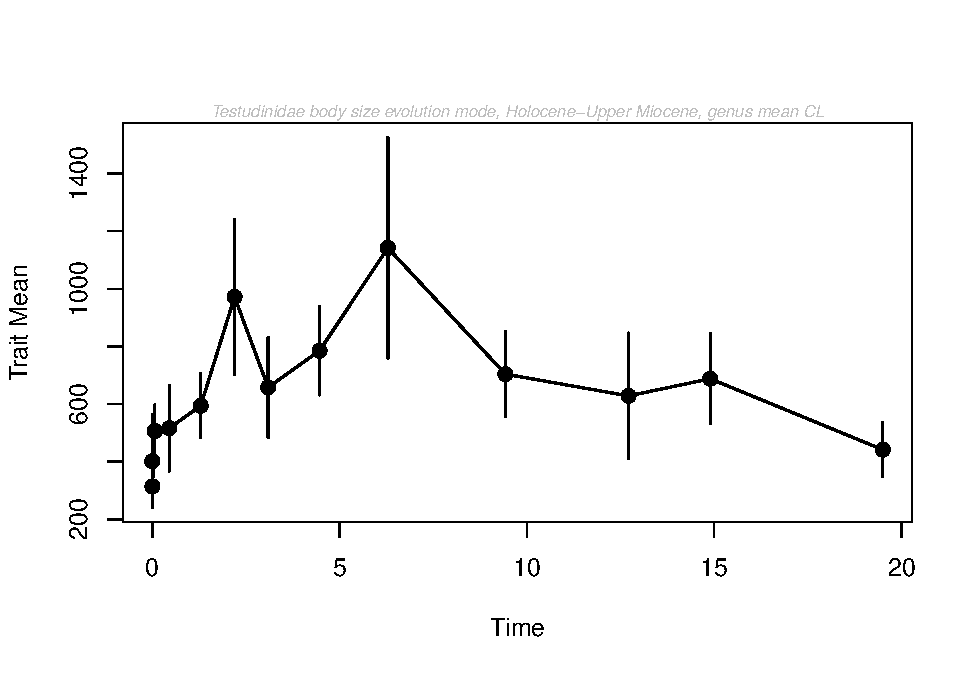
\includegraphics{MA_JJ_files/figure-latex/paleoTSAll-1.pdf}
	\caption{paleoTS plot with genus mean, all}
	\label{fig:pTSall}
\end{figure}

\begin{longtable}[]{@{}lrrrr@{}}
	\caption{Model-fitting results for testudinidae, genera,
		all}
	\label{tab:pTSallEM}\tabularnewline
	\toprule
	& logL & K & AICc & Akaike.wt\tabularnewline
	\midrule
	\endfirsthead
	\toprule
	& logL & K & AICc & Akaike.wt\tabularnewline
	\midrule
	\endhead
	GRW & -81.31790 & 2 & 167.9691 & 0.161\tabularnewline
	URW & -82.05721 & 1 & 166.5144 & 0.332\tabularnewline
	Stasis & -80.16802 & 2 & 165.6694 & 0.507\tabularnewline
	\bottomrule
\end{longtable}

\FloatBarrier
%__________________________________________________________________________

\subsubsection{continental dataset (excluding insular
	species)}\label{continental-excluding-insular-species}


\begin{figure}[H]
	\centering
	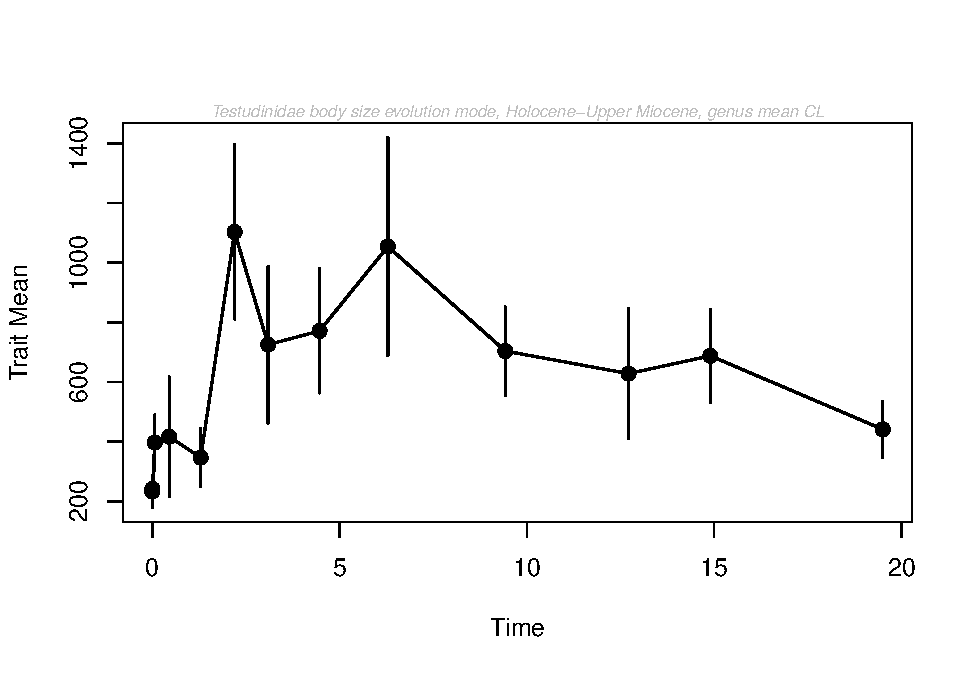
\includegraphics{MA_JJ_files/figure-latex/paleoTSC-1.pdf}
	\caption{paleoTS plot with genus mean, continental}
	\label{fig:pTSC}
\end{figure}

\begin{longtable}[]{@{}lrrrr@{}}
	\caption{Model-fitting results for testudinidae, genera,
		continental}
	\label{tab:pTSCEM}\tabularnewline
	\toprule
	& logL & K & AICc & Akaike.wt\tabularnewline
	\midrule
	\endfirsthead
	\toprule
	& logL & K & AICc & Akaike.wt\tabularnewline
	\midrule
	\endhead
	GRW & -82.26287 & 2 & 169.8591 & 0.300\tabularnewline
	URW & -83.12577 & 1 & 168.6515 & 0.548\tabularnewline
	Stasis & -82.93984 & 2 & 171.2130 & 0.152\tabularnewline
	\bottomrule
\end{longtable}


\FloatBarrier
%__________________________________________________________________________

\subsubsection{insular dataset (excluding
	continental)}\label{insular-excluding-continental}




\begin{figure}[H]
	\centering
	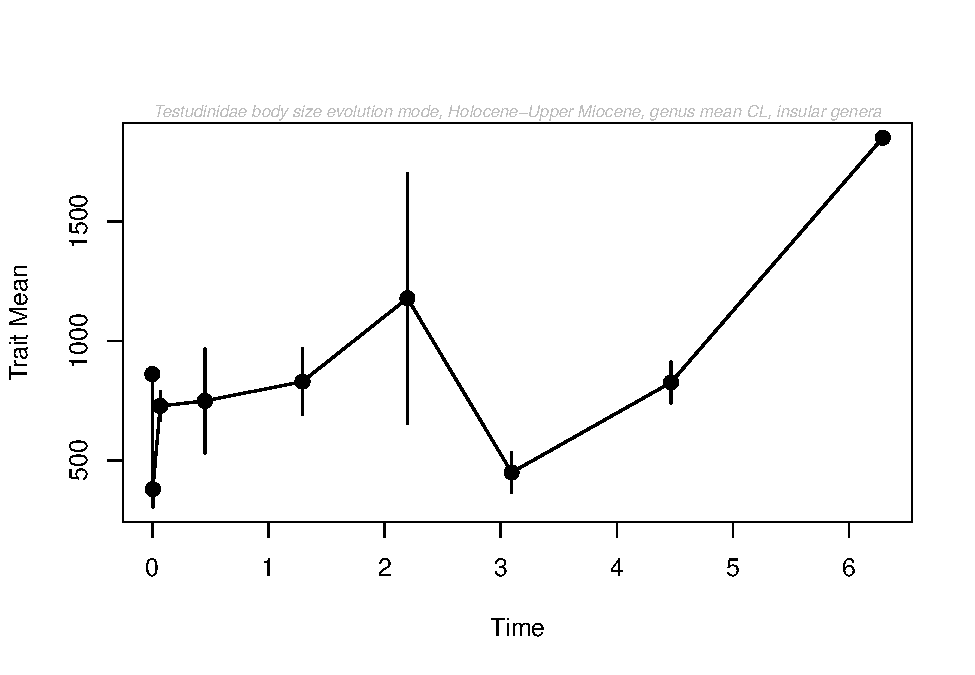
\includegraphics{MA_JJ_files/figure-latex/paleoTSI-1.pdf}
	\caption{paleoTS plot with genus mean, insular}
	\label{fig:pTSI}
\end{figure}

\begin{longtable}[]{@{}lrrrr@{}}
	\caption{Model-fitting results for testudinidae, genera,
		insular}
	\label{tab:pTSIEM}\tabularnewline
	\toprule
	& logL & K & AICc & Akaike.wt\tabularnewline
	\midrule
	\endfirsthead
	\toprule
	& logL & K & AICc & Akaike.wt\tabularnewline
	\midrule
	\endhead
	GRW & -68.57344 & 2 & 143.5469 & 0\tabularnewline
	URW & -75.76576 & 1 & 154.1982 & 0\tabularnewline
	Stasis & -60.41581 & 2 & 127.2316 & 1\tabularnewline
	\bottomrule
\end{longtable}

\FloatBarrier
%__________________________________________________________________________

\subsubsection{per continent}\label{per-continent}

\paragraph{Europe, genera}\label{europe-genera}

When repeating the analysis for European taxa only, all three groups -- complete, continental and insular data -- are best described by stasis with a model support between 92\,-\,99\,\% (Fig. \ref{fig:pTSEu}, \ref{fig:pTSEuC}, \ref{fig:pTSEuI}; Tables \ref{tab:pTSEuEM}, \ref{tab:pTSEuCEM}, \ref{tab:pTSEuIEM}).

\begin{figure}[H]
	\centering
	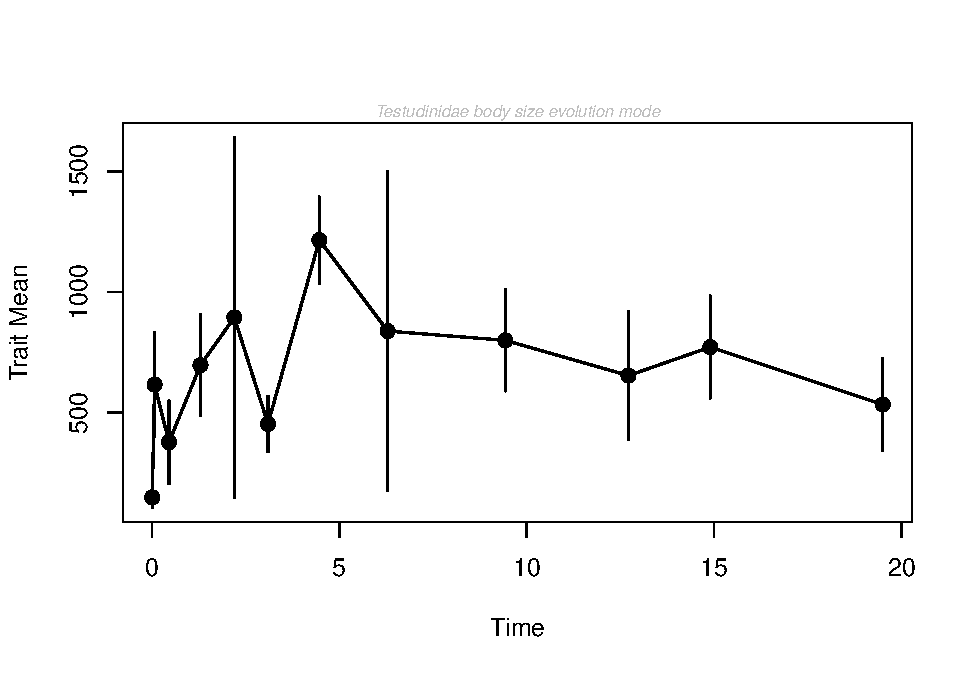
\includegraphics{MA_JJ_files/figure-latex/paleoTSEurope-1.pdf}
	\caption{Genera, Europe}
	\label{fig:pTSEu}
\end{figure}

\begin{longtable}[]{@{}lrrrr@{}}
	\caption{Model-fitting results for testudinidae, genera,
		Europe}
	\label{tab:pTSEuEM}\tabularnewline
	\toprule
	& logL & K & AICc & Akaike.wt\tabularnewline
	\midrule
	\endfirsthead
	\toprule
	& logL & K & AICc & Akaike.wt\tabularnewline
	\midrule
	\endhead
	GRW & -84.14010 & 2 & 173.7802 & 0.006\tabularnewline
	URW & -85.90727 & 1 & 174.2590 & 0.005\tabularnewline
	Stasis & -79.01365 & 2 & 163.5273 & 0.990\tabularnewline
	\bottomrule
\end{longtable}

\FloatBarrier
%__________________________________________________________________________



\paragraph{Eurasia,	genera}\label{eurasia-genera}


For Eurasia, the entire data as well as continental genera are best described by the unbiased random walk, although the model support is weak again. Continental species still have a better support (78\,\%; Fig. \ref{fig:pTSEsC}, Table \ref{tab:pTSEsCEM}) than all Eurasian data with only 56 \% (Fig. \ref{fig:pTSEs}, Table \ref{tab:pTSEsEM}). Insular Eurasian species, however, conform to stasis again, although with lower support values (68\,\%; Fig. \ref{fig:pTSEsI}, Table \ref{tab:pTSEsIEM}).



\begin{figure}[H]
	\centering
	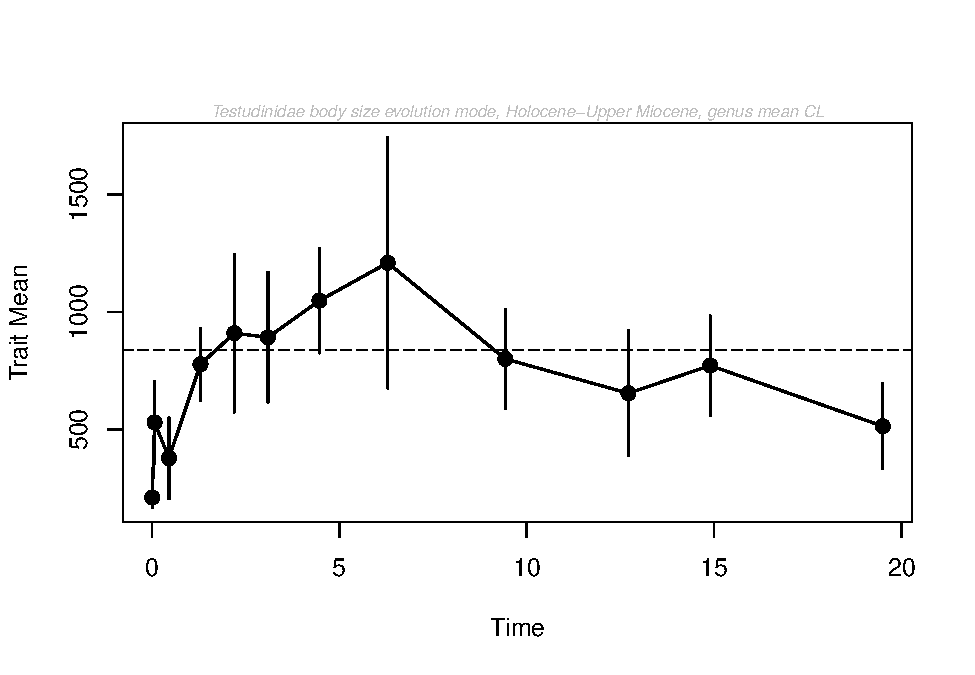
\includegraphics{MA_JJ_files/figure-latex/paleoTSEurasia-1.pdf}
	\caption{paleoTS, genera, Eurasia}
	\label{fig:pTSEs}
\end{figure}

\begin{longtable}[]{@{}lrrrr@{}}
	\caption{Model-fitting results for testudinidae, genera,
		Eurasia}
	\label{tab:pTSEsEM}\tabularnewline
	\toprule
	& logL & K & AICc & Akaike.wt\tabularnewline
	\midrule
	\endfirsthead
	\toprule
	& logL & K & AICc & Akaike.wt\tabularnewline
	\midrule
	\endhead
	GRW & -85.25195 & 2 & 175.8372 & 0.149\tabularnewline
	URW & -85.39072 & 1 & 173.1814 & 0.562\tabularnewline
	Stasis & -84.58890 & 2 & 174.5111 & 0.289\tabularnewline
	\bottomrule
\end{longtable}



\FloatBarrier
%__________________________________________________________________________


\newpage
\section{Discussion}

\subsection{Completeness of data set}

completeness of data set/benefits of additional sampling (SACs)
- how much of the "actual" data is represented by our data set?

- how many species/genera are there, how many are present in my data set?
lapparent de broin, 2001 + rhodin et al., 2015
--> check turtles of the world checklist, how many extant genera + species?


\subsection{Population structure?}

As has been reported for many animals, 

- compare with Lyons and Smith, 2010 (mammals though, but)
- is there a study about population structure in testudinidae?
- kozlowski and gawelczyk, 2002 --> body size distributions usually right-skewed

\subsection{Time-scale analysis}

--> what does model support depend on? what does a relatively low model support mean?


% LIMITATIONS
%\todo{add at some point that phylogenetics were not considered because not enough data for fossil species --> or only in discussion? full-evidence analysis would be nice as in Slater et al., 2017 (baleen whales) --> cite Lapparent de Broin, 2006 + 2001: phylogenetic relationships between genera are not definitely established, }


- study would benefit from more sampling! (SAC, model supports paleoTS)

- include more data, not only literature but actually measure shells/other skeletal elements --> maybe gather further data to more reliably estimate body sizes

- include shapes/geometric morphometrics --> volume/body mass?

- paleoTS --> is designed to deal with incomplete data (FOSSIL)

- unbiased random walk on continents --> CL fluctuates more than on islands --> "giant" forms completetely disappeared in comparison to insular species

- what can influence distribution: climate, selective pressures, diet, intra-specific competition (Madagascar)

- I guess: climate affects body size reduction, but extinctions were human-driven
--> Aldabra/Galapagos (whaling industry)
--> mammal megafauna was hunted to extinction by humans




%____________________________________________________

Aldabra tortoise: no evidence of size increase, probably originate from giant continental tortoises (large tortoises are able to float: bouyancy and fasting endurance)

- Meiolania --> study that they were extirpated by humans?

%___________________________
\subsection{Conclusion}


This study would definitely benefit from further sampling, ideally by directly measuring fossil specimens in museum collections.

beyond literature research but actual measurements of museum collections, especially on the continents other than Europe. Possibly, a nearly complete (as complete as it can be, based on fossils) dataset could be achieved, if estimates based on single scutes/shell fragments could be established.

Giant tortoises seem to occupy only a small temperature range, since they are in danger of overheating (...), but also cannot cope with cold winters (...). However, obviously appropriate climates are still available, since giant tortoises are still present in some places, which means climate alone cannot have driven the extinction, at least not on tropical islands.
I would assume, that climate drove some decrease in body size (as exemplified by Gopherus agassizi (...) and Cherins angulata), although in the last example the size decrease has been labeled human-induced (since large individuals are hunted more frequently, shifting the body size distribution to the smaller scale).


- studies on individual species which seem to decrease in size: gopherus und chersina angulata --> stone age

- smith et al., 2016: on higher taxa level, most groups seem to conform to the null model (changes occur on species level, display trends, but no tendencies)

%Smith et al., 2016
%As drawn, there is no upward tendency, as increases and decreases in size are equally frequent. This is the pattern expected in the null case with no evolutionary forces acting at the scale of the lineage. Notice, however, that there is nevertheless a trend—a trend in the maximum. The distinction is that “tendency” refers to the pattern of change at the lower level, in this case the species level, whereas “trend” refers to a change in a summary statistic at the clade level, in this case an increase in the clademaximum.Other summary statistics of interest include the mean, median, and minimum. Thus, there is not necessarily a connection between tendency and trend: One can have a trend without a tendency. For body size evolution in particular, the most commonly observed and documentable kind of trend—a rise in the maximum—does not by itself tell us much about underlying tendencies. Maxima are expected to increase even if no tendencies, no evolutionary forces, are present. Thus, we cannot infer the existence of a selective advantage of large size merely from an increase in the maximum. The

would be interesting to investigate body size trends for individual genera or even species, for this further sampling is needed. use ancestor-descendant data! 
some pap

\newpage
%\bibliography{file}
\FloatBarrier
\begin{appendices}
%\section{Appendix}
\section{Sampling accumulation curves}

\begin{center}
	\begin{figure}[H]
		\subfloat[Species per locality]{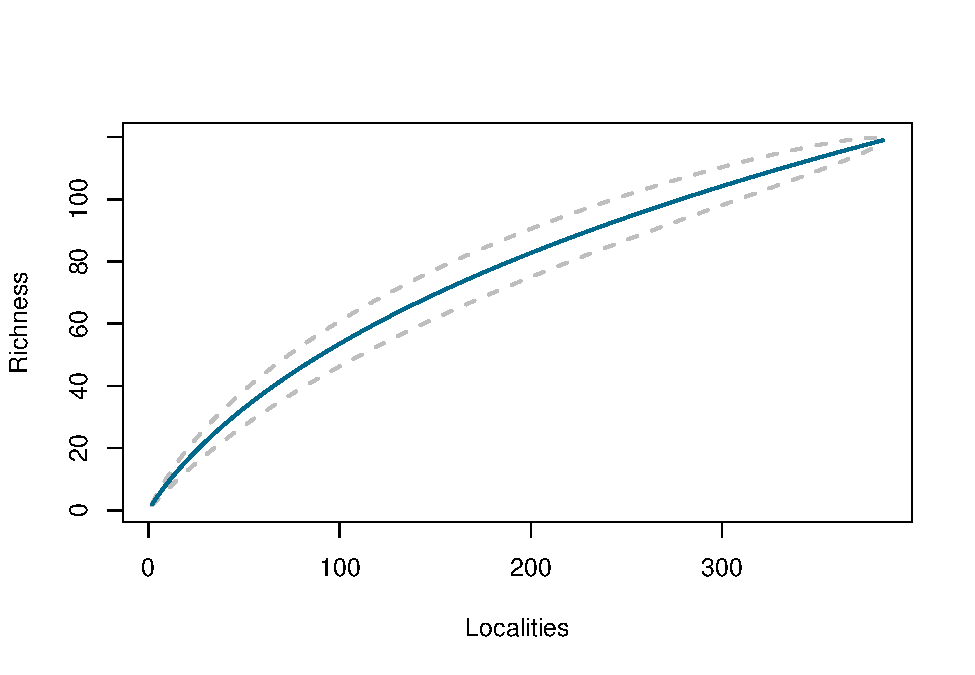
\includegraphics[scale=0.3]{MA_JJ_files/figure-latex/SACSpecies-1.pdf}}
		\subfloat[Species per reference]{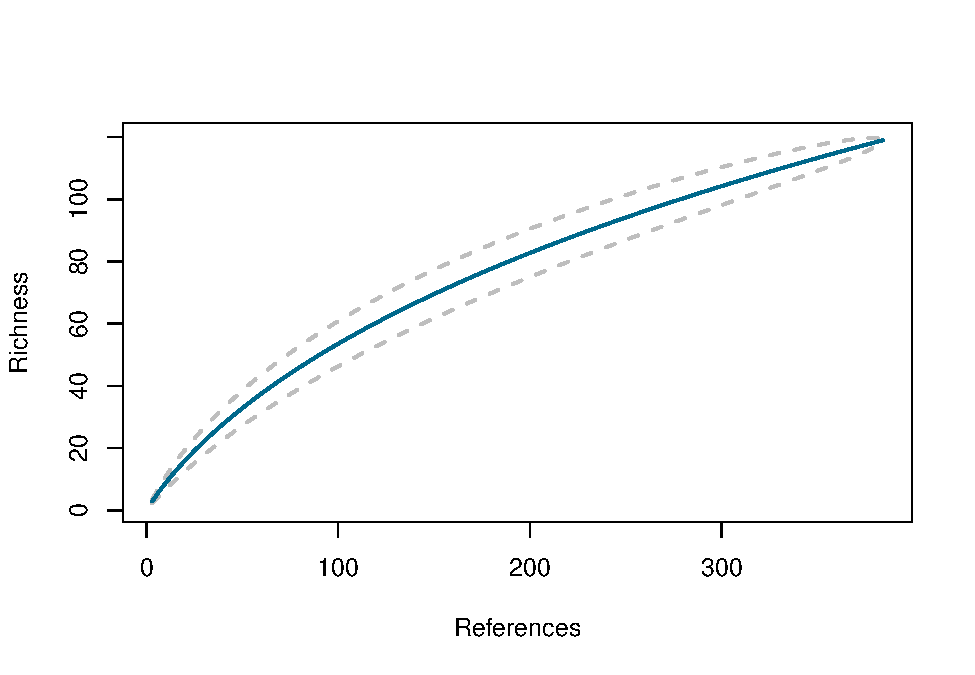
\includegraphics[scale=0.3]{MA_JJ_files/figure-latex/SACSpecies-2.pdf}}	\subfloat[Africa]{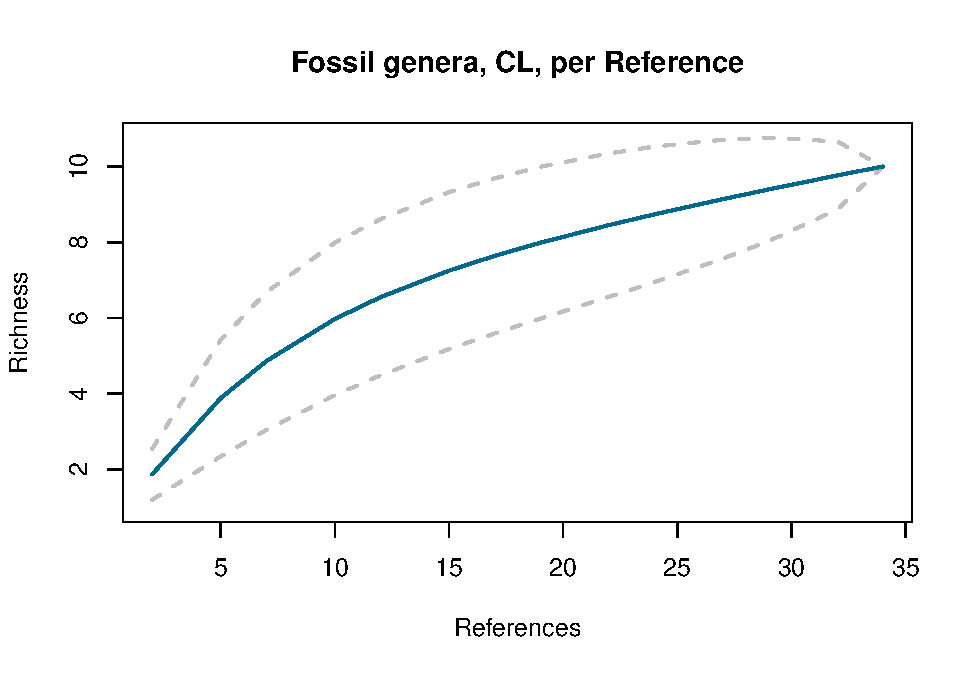
\includegraphics[scale=0.3]{MA_JJ_files/figure-latex/SACGAfrica-1.pdf}}
		\hfill %
		\subfloat[America]{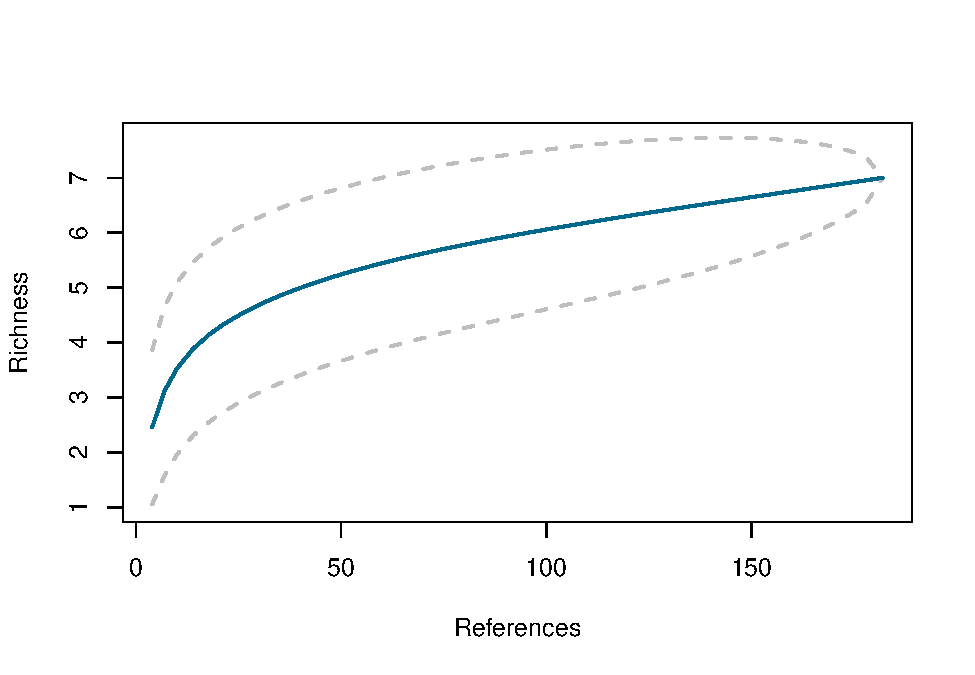
\includegraphics[scale=0.3]{MA_JJ_files/figure-latex/SACGAmerica-1.pdf}}
		\subfloat[North America]{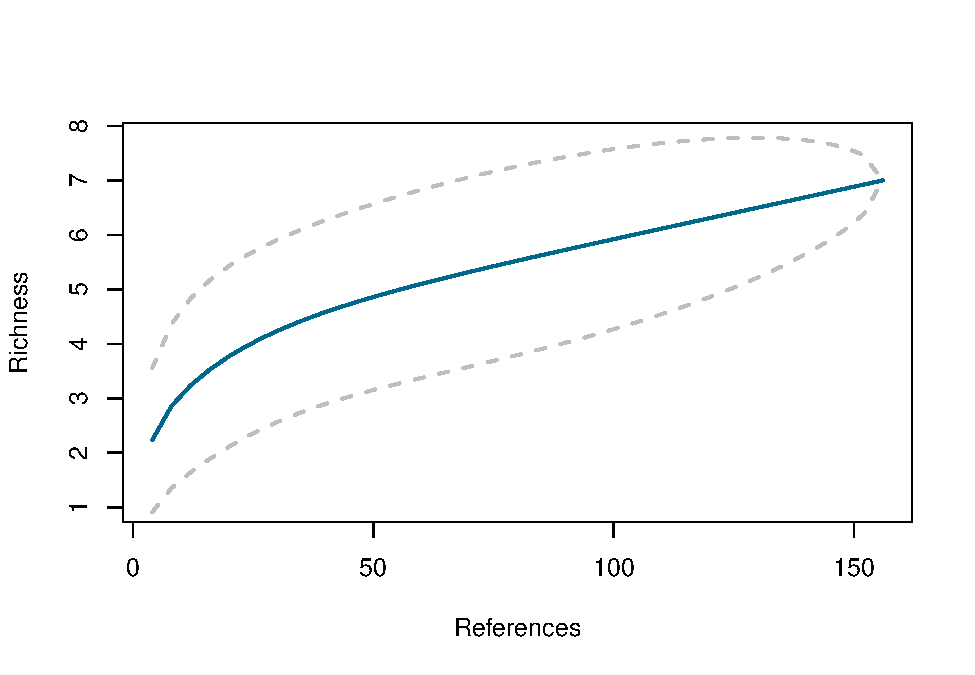
\includegraphics[scale=0.3]{MA_JJ_files/figure-latex/SACGNAmerica-1.pdf}}
		\subfloat[South America]{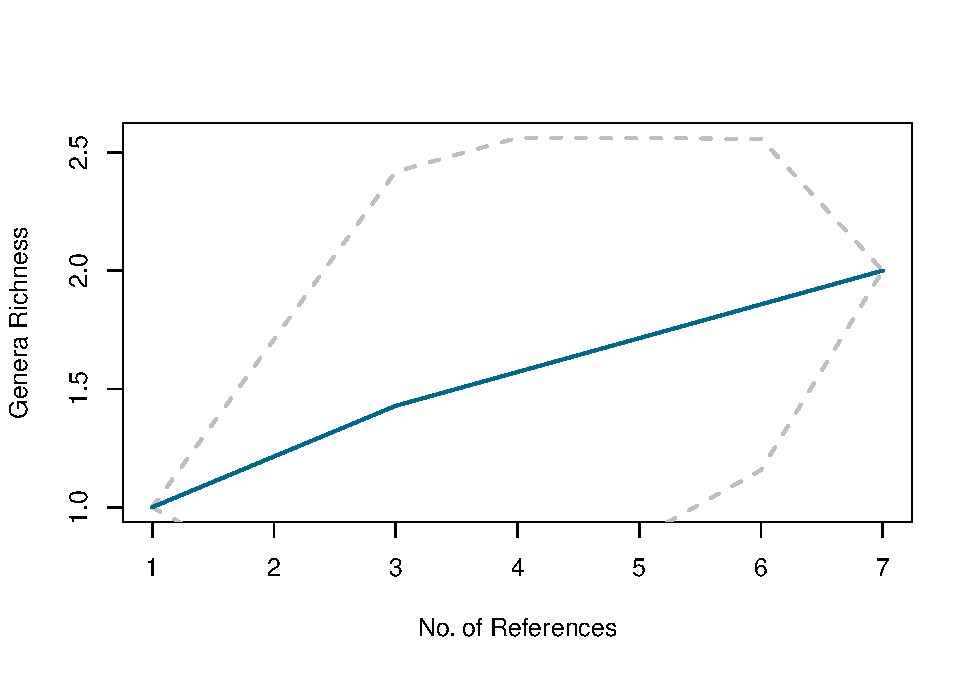
\includegraphics[scale=0.3]{MA_JJ_files/figure-latex/SACGSAmerica-1.pdf}}
		\hfill %
		\subfloat[Asia]{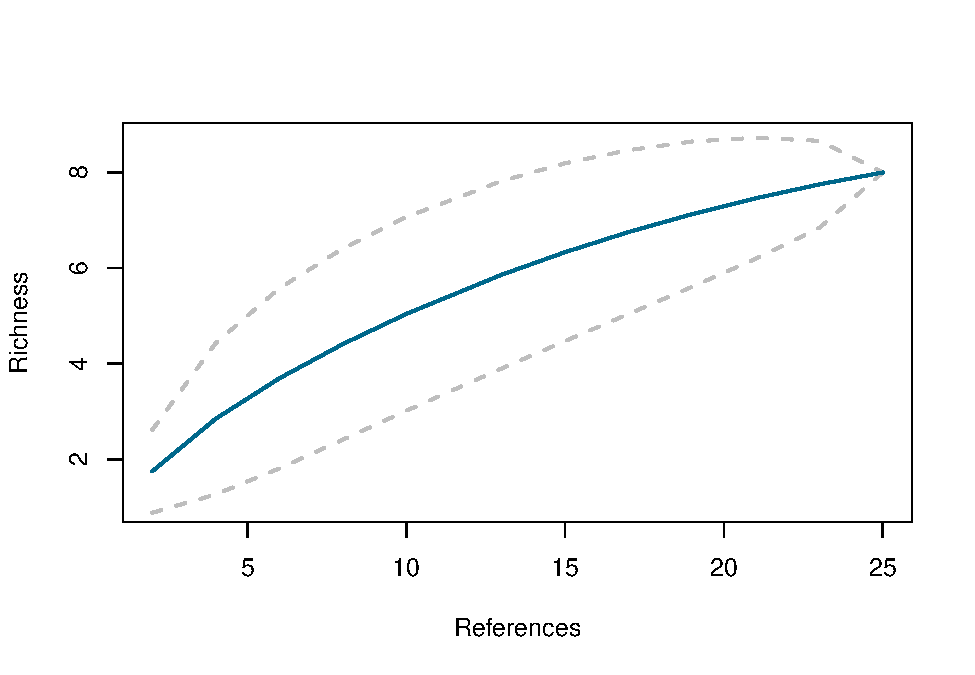
\includegraphics[scale=0.3]{MA_JJ_files/figure-latex/SACGAsia-1.pdf}}
		\subfloat[Europe]{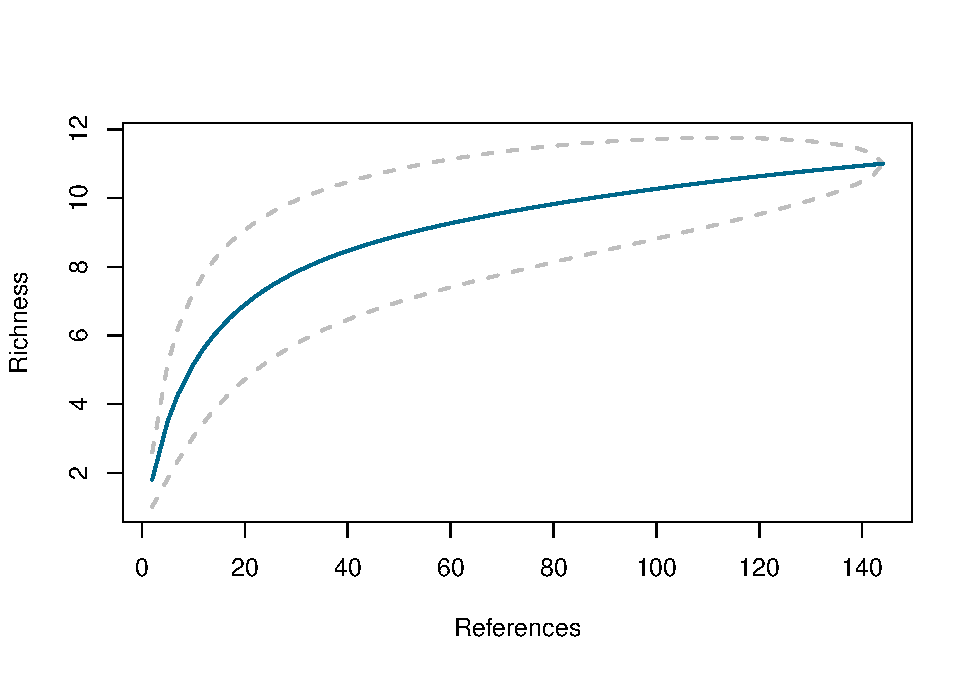
\includegraphics[scale=0.3]{MA_JJ_files/figure-latex/SACGEurope-1.pdf}}
		\subfloat[Eurasia]{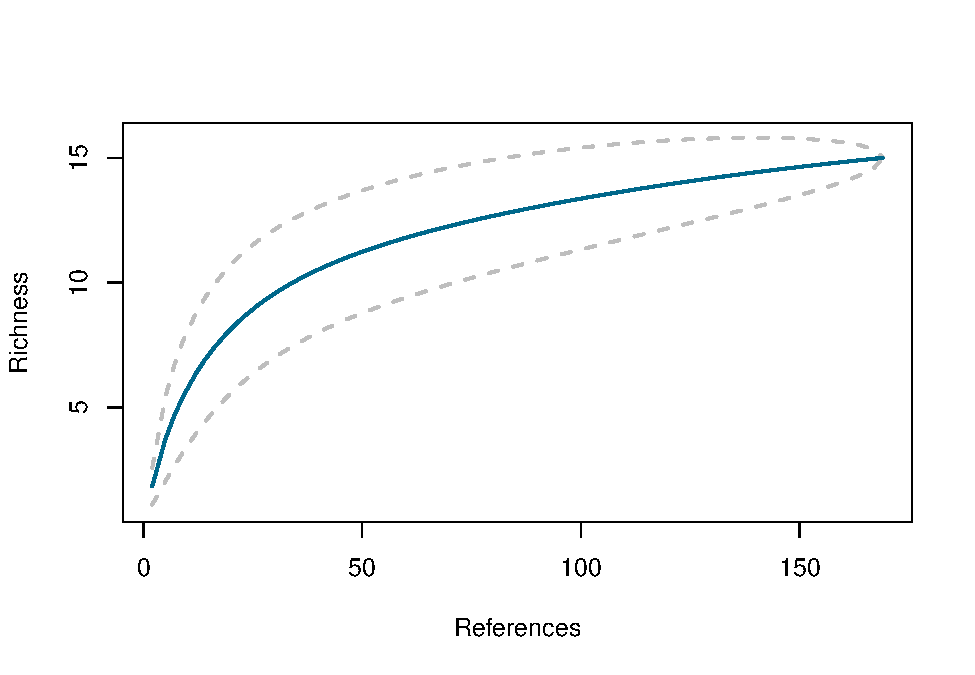
\includegraphics[scale=0.3]{MA_JJ_files/figure-latex/SACGEurasia-1.pdf}}
		\caption[Additional sampling accumulation curves]{Sampling accumulation curves: (a) - (b) Species are not sufficiently sampled, regardless of sampling unit. (c) - (i) Sampling Accumulation Curves on generic level per continent. Only Europe (h) and Eurasia (i) are sufficiently sampled. Dashed lines represent the confidence interval.}
		\label{fig:SACall}
	\end{figure}
\end{center}

\FloatBarrier


\begin{longtable}[]{@{}llllllll@{}}
	\caption{Genera abundance across the continents.}
	\label{tab:SAC}
	\toprule
	Genus & Africa.x & America & N-America & S-America & Asia.x & Europe.x &
	n\tabularnewline
	\midrule
	\endhead
	Aldabrachelys & 4 & - & - & - & 2 & - & 2\tabularnewline
	Caudochelys & - & 4 & 4 & - & - & - & -\tabularnewline
	Centrochelys & 2 & - & - & - & - & 12 & 12\tabularnewline
	Cheirogaster & - & - & - & - & - & 9 & 9\tabularnewline
	Chelonoidis & - & 28 & - & 6 & - & - & -\tabularnewline
	Ergilemys & - & - & - & - & 2 & 3 & 4\tabularnewline
	Eurotestudo & - & - & - & - & - & 10 & 10\tabularnewline
	Geochelone & 4 & 10 & 8 & 1 & 1 & 2 & 3\tabularnewline
	Gopherus & - & 92 & 88 & - & - & - & -\tabularnewline
	``Hadrianus'' & - & - & - & - & - & 1 & 1\tabularnewline
	Hesperotestudo & - & 46 & 43 & - & - & - & -\tabularnewline
	Homopus & 1 & - & - & - & - & - & -\tabularnewline
	Impregnochelys & 1 & - & - & - & - & - & -\tabularnewline
	Indotestudo & - & - & - & - & 1 & - & 1\tabularnewline
	Kinixys & 1 & - & - & - & - & - & -\tabularnewline
	Manouria & - & - & - & - & 2 & - & 2\tabularnewline
	Megalochelys & - & - & - & - & 12 & - & 12\tabularnewline
	Mesocherus & 5 & - & - & - & - & - & -\tabularnewline
	Namibchersus & 9 & - & - & - & - & - & -\tabularnewline
	Paleotestudo & - & - & - & - & - & 26 & 26\tabularnewline
	Psammobates & 1 & - & - & - & - & - & -\tabularnewline
	Stylemys & - & 1 & 1 & - & - & - & -\tabularnewline
	Taraschelon & - & - & - & - & - & 1 & 1\tabularnewline
	Testudo & 5 & 1 & 1 & - & 4 & 51 & 54\tabularnewline
	Titanochelon & - & - & - & - & - & 22 & 22\tabularnewline
	gen. & - & - & - & - & 1 & 7 & 8\tabularnewline
	\bottomrule
\end{longtable}

\newpage
\section{Histograms}


\begin{center}
	\begin{figure}[H]
		\subfloat[Raw data]{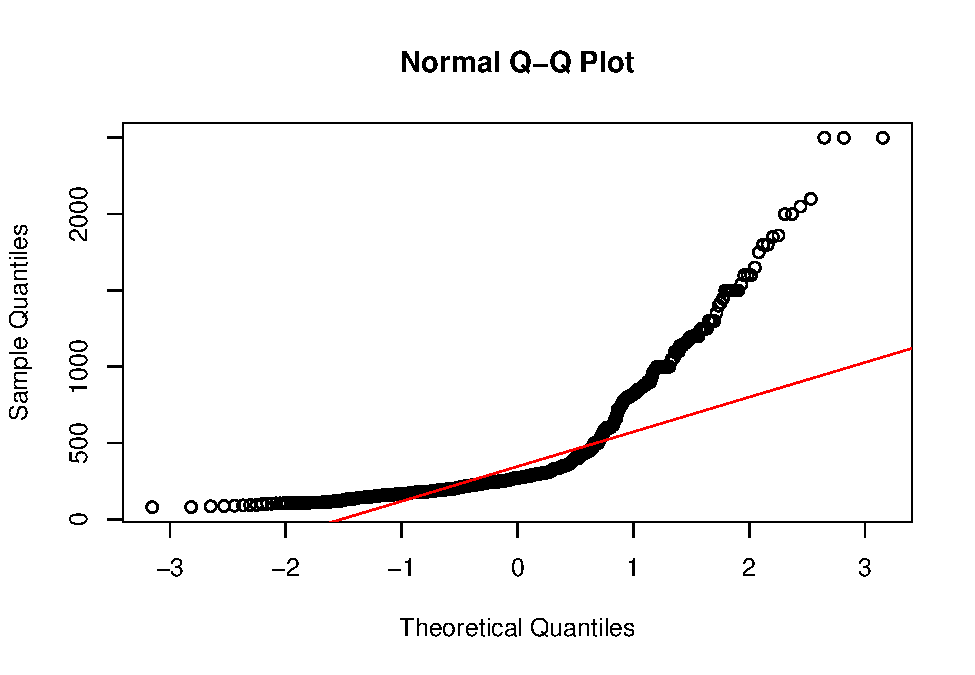
\includegraphics[scale=0.45]{MA_JJ_files/figure-latex/normalDistribution-1.pdf}}
		\subfloat[Logtransformed data]{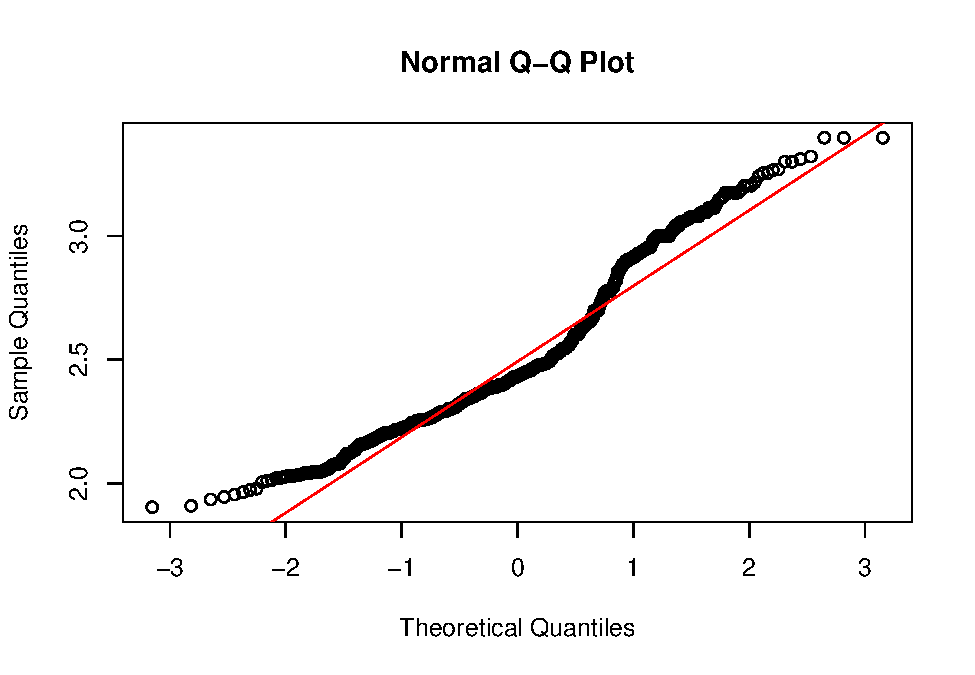
\includegraphics[scale=0.45]{MA_JJ_files/figure-latex/normalDistribution-2.pdf}}	
		\caption[Testing normal distribution]{Visual test for normal distribution. In case of normally distributed data, the black circles should follow the red line, which is not the case for either raw data (a) nor logtransformed data (b). Therefore, data is not normally distributed.}
		\label{fig:NormDis}
	\end{figure}
\end{center}


\begin{center}
	\begin{figure}[H]
		\subfloat[Fossil vs. modern, continental vs. insular]{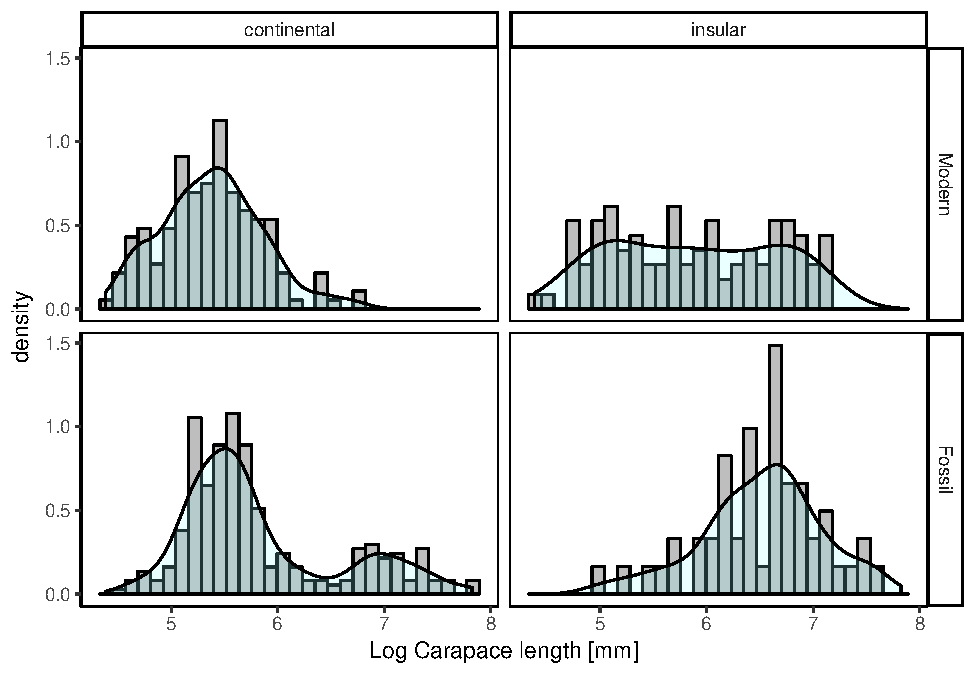
\includegraphics[scale=0.45]{MA_JJ_files/figure-latex/HistFMCI-1.pdf}}
		\subfloat[Per continent]{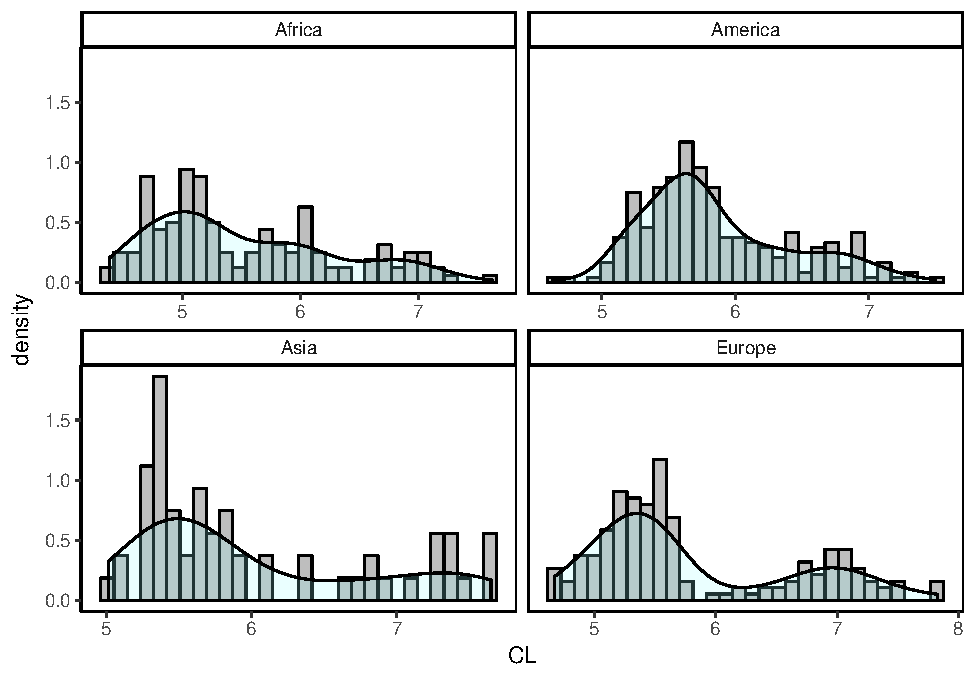
\includegraphics[scale=0.45]{MA_JJ_files/figure-latex/HistCon-1.pdf}}	
		\caption[Additional histograms]{Histograms for several subgroups of the dataset.}
		\label{fig:HistRest}
	\end{figure}
\end{center}
\section*{Boxplots}
\section{Random Sampling}


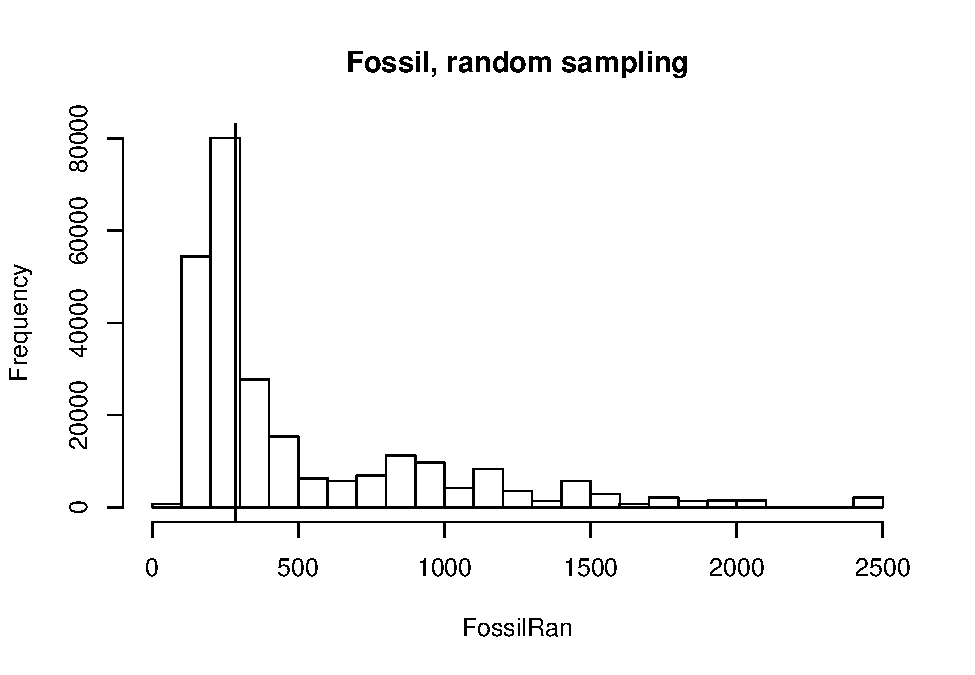
\includegraphics{MA_JJ_files/figure-latex/RSFM-1.pdf}


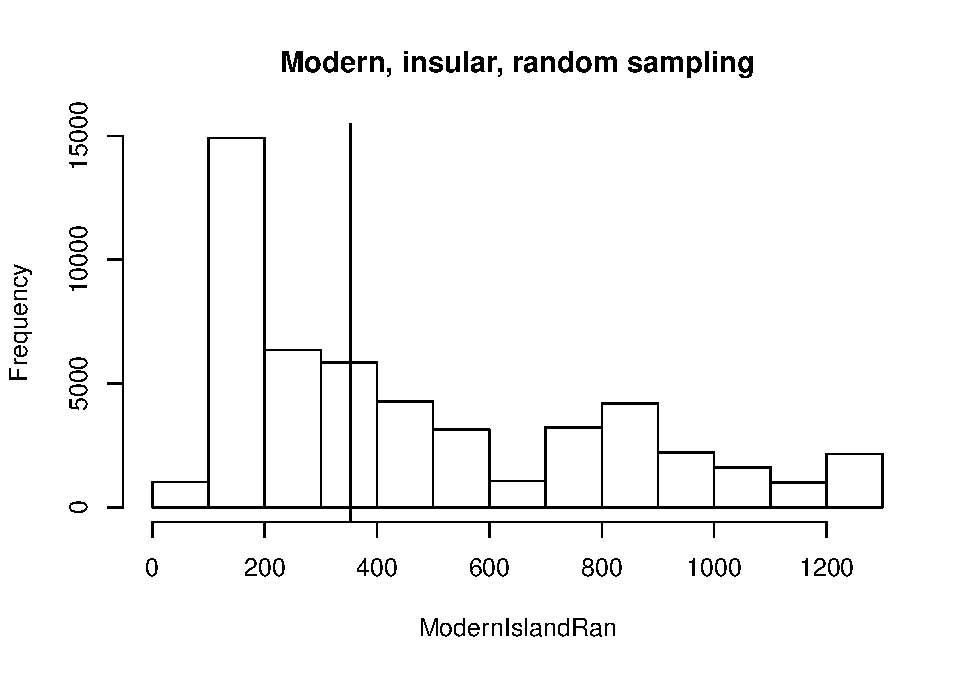
\includegraphics{MA_JJ_files/figure-latex/RSMFCI-1.pdf}


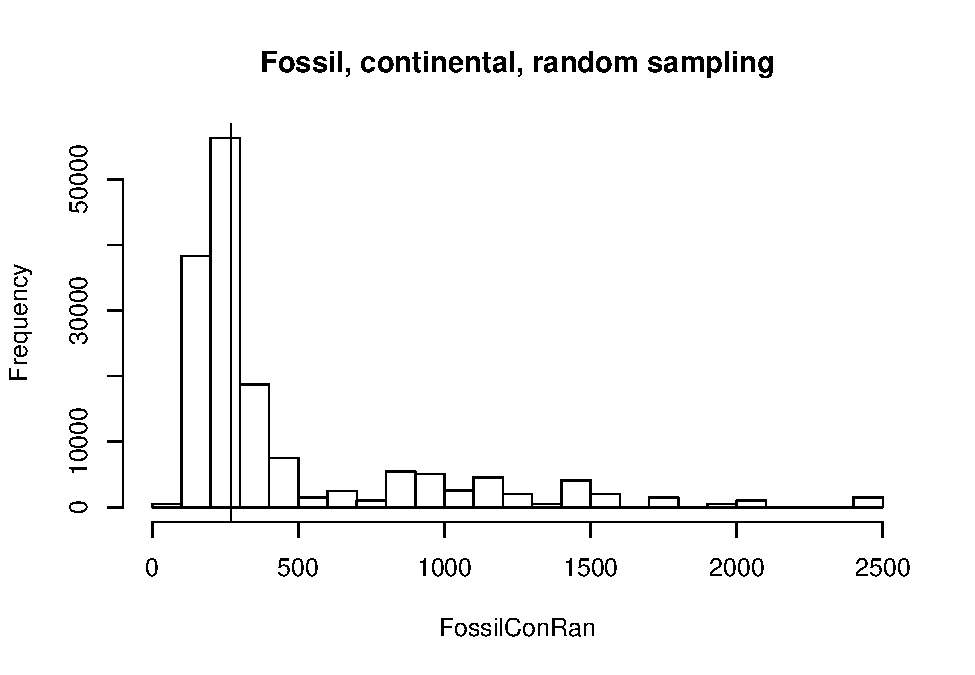
\includegraphics{MA_JJ_files/figure-latex/RSMFCI-2.pdf}



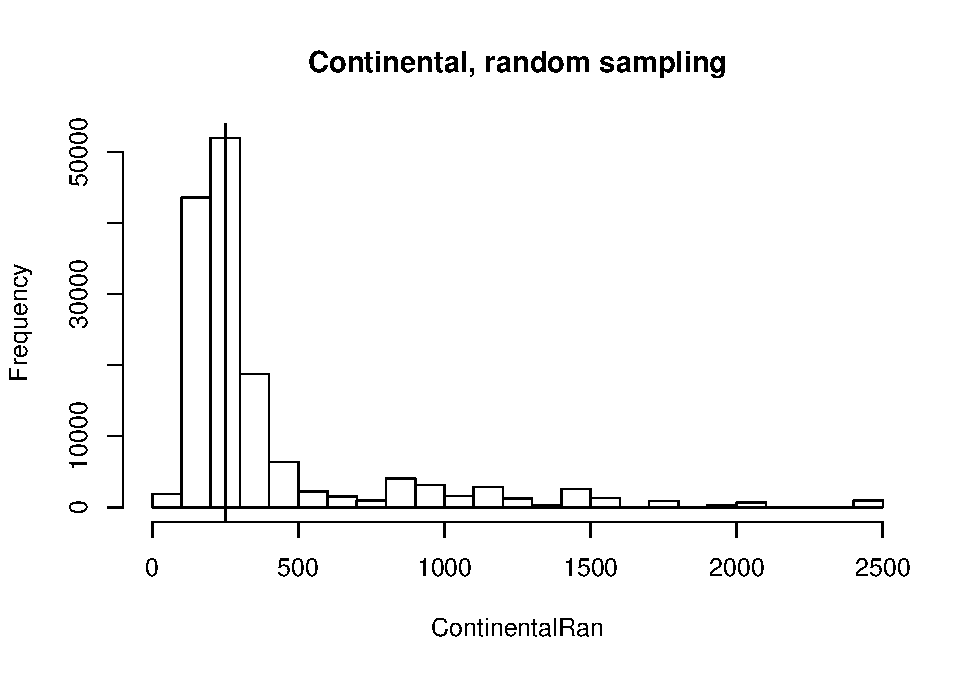
\includegraphics{MA_JJ_files/figure-latex/RSCI-1.pdf}



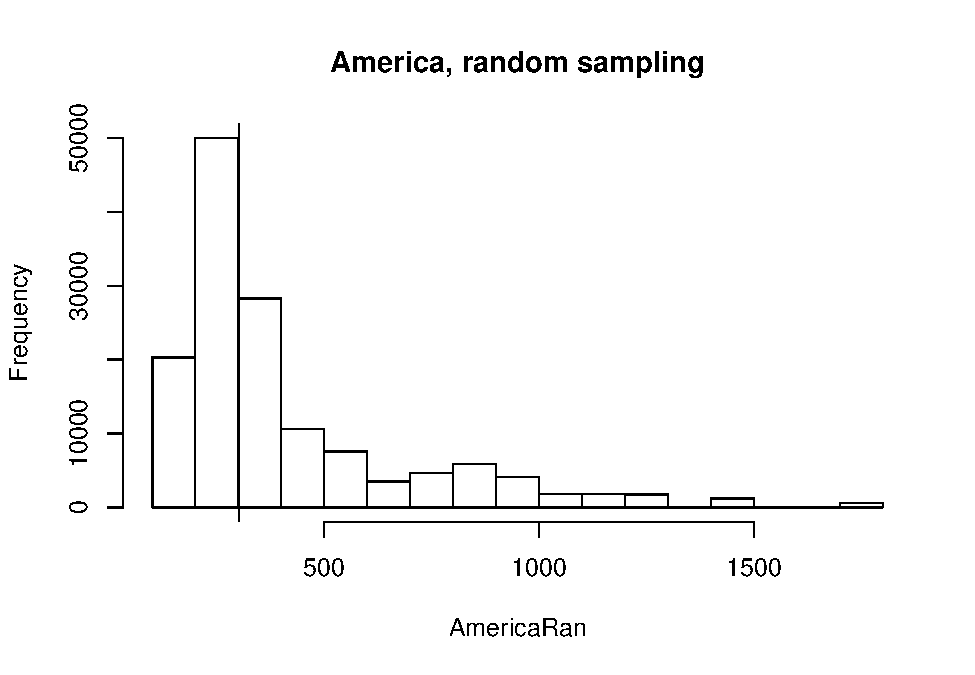
\includegraphics{MA_JJ_files/figure-latex/RSCon-1.pdf}
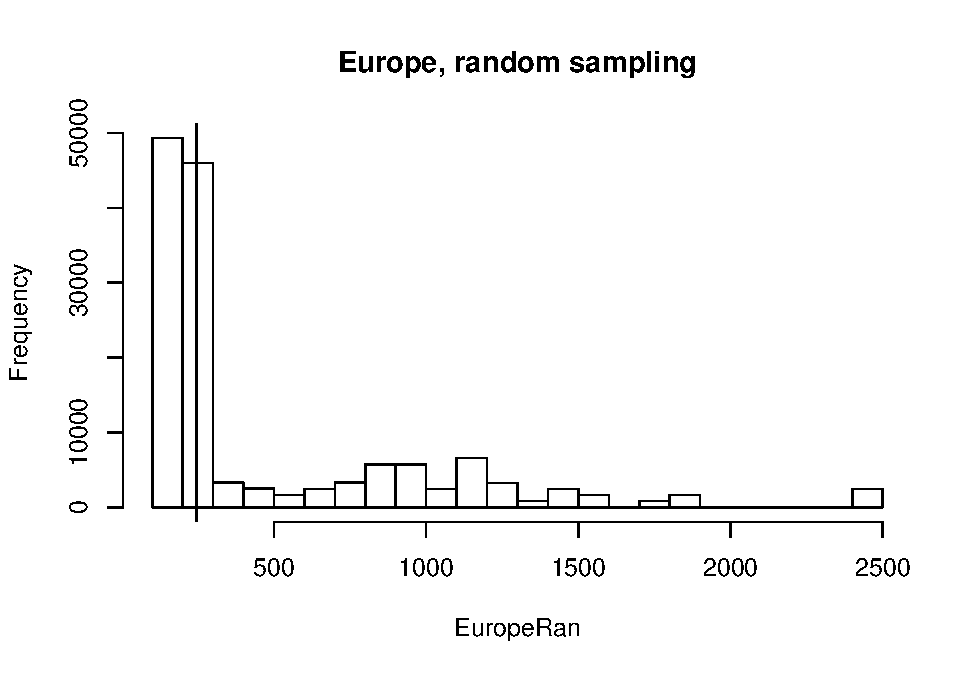
\includegraphics{MA_JJ_files/figure-latex/RSCon-2.pdf}
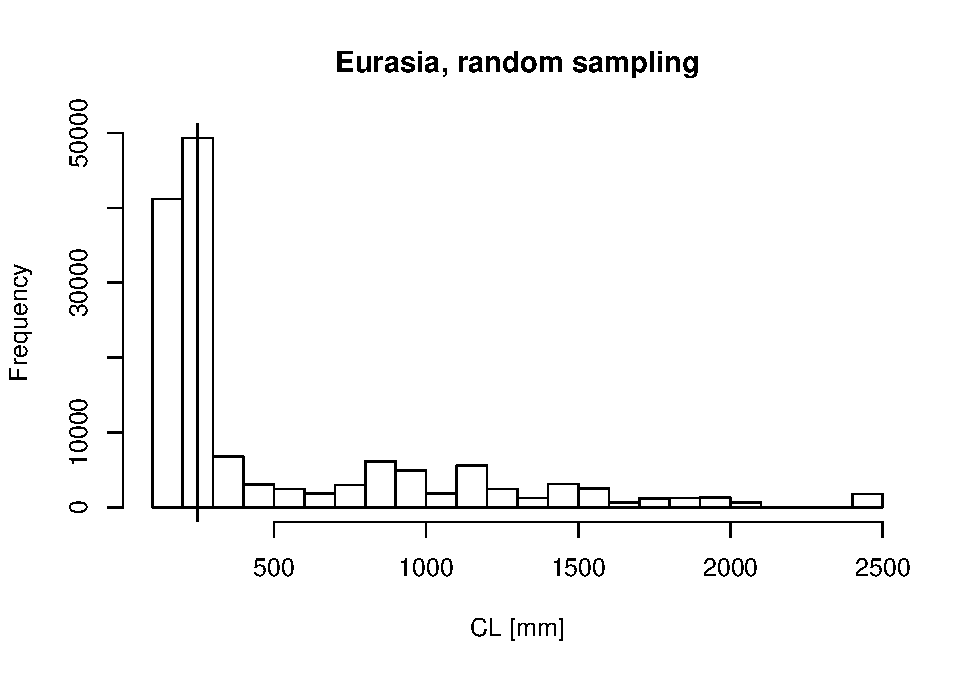
\includegraphics{MA_JJ_files/figure-latex/RSCon-3.pdf}
\section{Tables}

\begin{landscape}
\begin{longtable}[]{@{}rrrrrrrrrrrrl@{}}
	\caption[General statistics]{General statistics of body size data: all, per time bin,
		insular and continental, per continent (all referring to CL: min, max,
		variance, mean, logmean, median, logmedian, skewness, logskewness,
		kurosis, logkurtosis}
	\label{tab:stats}\tabularnewline
	\toprule
	nCL & min & max & var & mean & logm & med & logmed & skew & logsk & kurt
	& logku & Variable\tabularnewline
	\midrule
	\endfirsthead
	\multicolumn{4}{c}%
	{\tablename\ \thetable\ -- \textit{continued from previous page}}\tabularnewline
	\toprule
	nCL & min & max & var & mean & logm & med & logmed & skew & logsk & kurt
	& logku & Variable\tabularnewline
	\midrule
	\endhead
	616 & 80.00 & 2500 & 164537.80 & 437.2 & 2.5 & 270.5 & 2.4 & 2.14 & 0.69
	& 8.00 & 2.73 & all\tabularnewline
	253 & 80.00 & 1300 & 67485.50 & 330.3 & 2.4 & 242.0 & 2.4 & 1.83 & 0.58
	& 5.87 & 2.69 & Modern\tabularnewline
	49 & 102.44 & 1250 & 69690.66 & 445.9 & 2.6 & 334.7 & 2.5 & 1.20 & 0.24
	& 3.61 & 2.56 & Upper Pleistocene\tabularnewline
	53 & 132.00 & 1800 & 97910.83 & 387.1 & 2.5 & 292.9 & 2.5 & 3.03 & 1.52
	& 12.24 & 5.55 & Middle Pleistocene\tabularnewline
	57 & 107.80 & 2000 & 161948.82 & 463.5 & 2.5 & 263.0 & 2.4 & 1.74 & 0.73
	& 5.76 & 2.40 & Lower Pleistocene\tabularnewline
	31 & 118.90 & 2050 & 411224.51 & 555.2 & 2.5 & 194.9 & 2.3 & 1.31 & 0.93
	& 3.12 & 2.11 & Gelasian\tabularnewline
	21 & 90.00 & 1600 & 270535.82 & 610.6 & 2.6 & 428.0 & 2.6 & 1.00 & 0.14
	& 2.50 & 1.99 & Piacencian\tabularnewline
	26 & 176.00 & 2500 & 476162.71 & 955.2 & 2.9 & 857.5 & 2.9 & 1.11 &
	-0.40 & 3.56 & 2.30 & Zanclean\tabularnewline
	10 & 140.00 & 2100 & 602611.21 & 948.9 & 2.8 & 916.0 & 2.9 & 0.26 &
	-0.22 & 1.49 & 1.29 & Messinian\tabularnewline
	45 & 107.00 & 1540 & 175470.12 & 462.7 & 2.5 & 250.0 & 2.4 & 1.49 & 0.81
	& 3.74 & 2.54 & Tortonian\tabularnewline
	27 & 111.00 & 1500 & 126060.40 & 337.7 & 2.4 & 220.0 & 2.3 & 2.49 & 1.77
	& 7.77 & 5.30 & Serravallian\tabularnewline
	14 & 270.00 & 1600 & 230451.33 & 747.9 & 2.8 & 700.0 & 2.8 & 0.30 & 0.03
	& 1.55 & 1.18 & Langhian\tabularnewline
	30 & 113.00 & 1100 & 76288.76 & 406.8 & 2.5 & 302.4 & 2.5 & 1.27 & 0.45
	& 3.45 & 2.26 & Burdigalian/Aquitanian\tabularnewline
	253 & 80.00 & 1300 & 67485.50 & 330.3 & 2.4 & 242.0 & 2.4 & 1.83 & 0.58
	& 5.87 & 2.69 & Modern\tabularnewline
	363 & 90.00 & 2500 & 219004.66 & 511.7 & 2.6 & 285.6 & 2.5 & 1.83 & 0.68
	& 6.11 & 2.42 & Fossil\tabularnewline
	469 & 81.00 & 2500 & 157808.79 & 392.9 & 2.5 & 250.0 & 2.4 & 2.65 & 1.07
	& 10.57 & 3.74 & continental\tabularnewline
	147 & 80.00 & 2000 & 160834.35 & 578.5 & 2.6 & 500.0 & 2.7 & 1.02 &
	-0.27 & 3.95 & 2.05 & insular\tabularnewline
	157 & 81.00 & 830 & 17009.02 & 244.0 & 2.3 & 221.0 & 2.3 & 1.92 & 0.29 &
	8.09 & 2.98 & modern-con\tabularnewline
	96 & 80.00 & 1300 & 118641.09 & 471.5 & 2.6 & 353.0 & 2.5 & 0.82 & 0.01
	& 2.47 & 1.77 & modern-ins\tabularnewline
	312 & 90.00 & 2500 & 212116.79 & 467.9 & 2.5 & 270.0 & 2.4 & 2.11 & 0.96
	& 7.25 & 2.96 & fossil-con\tabularnewline
	51 & 150.00 & 2000 & 180825.40 & 780.0 & 2.8 & 750.0 & 2.9 & 1.11 &
	-0.40 & 4.02 & 3.18 & fossil-ins\tabularnewline
	142 & 80.00 & 2050 & 112417.26 & 347.7 & 2.4 & 193.5 & 2.3 & 2.10 & 0.68
	& 7.97 & 2.48 & Africa\tabularnewline
	242 & 102.44 & 1800 & 82209.71 & 415.0 & 2.5 & 302.2 & 2.5 & 1.92 & 0.75
	& 6.79 & 2.91 & America\tabularnewline
	59 & 150.00 & 2100 & 323123.20 & 585.5 & 2.6 & 280.0 & 2.4 & 1.43 & 0.85
	& 3.61 & 2.24 & Asia\tabularnewline
	173 & 107.00 & 2500 & 254222.84 & 491.2 & 2.5 & 245.0 & 2.4 & 1.86 &
	0.81 & 6.30 & 2.34 & Europe\tabularnewline
	\bottomrule
\end{longtable}
\end{landscape}

%\begin{longtable}[]{@{}llrr@{}}
	\caption[Species per time bins]{Overview over fossil species per time bin, with sample size and
		mean CL.}
	\label{tab:SpecBins}\tabularnewline
	\toprule
	EpochBins & Taxon & n & meanCL\tabularnewline
	\midrule
	\endfirsthead
	\toprule
	EpochBins & Taxon & n & meanCL\tabularnewline
	\midrule
	\endhead
	Upper Pleistocene & Centrochelys robusta & 1 & 850.0000\tabularnewline
	Upper Pleistocene & Chelonoidis denticulata & 1 &
	616.0000\tabularnewline
	Upper Pleistocene & Chelonoidis lutzae & 1 & 830.0000\tabularnewline
	Upper Pleistocene & Chelonoidis marcanoi & 4 & 672.2500\tabularnewline
	Upper Pleistocene & Chelonoidis monensis & 1 & 500.0000\tabularnewline
	Upper Pleistocene & Chelonoidis sombrerensis & 1 &
	990.0000\tabularnewline
	Upper Pleistocene & Chelonoidis sp. & 3 & 666.6667\tabularnewline
	Upper Pleistocene & Eurotestudo hermanni & 1 & 187.0000\tabularnewline
	Upper Pleistocene & gen. indet. & 1 & 813.0000\tabularnewline
	Upper Pleistocene & Geochelone sp. & 2 & 475.0000\tabularnewline
	Upper Pleistocene & Gopherus agassizi & 1 & 252.0000\tabularnewline
	Upper Pleistocene & Gopherus polyphemus & 20 & 292.9700\tabularnewline
	Upper Pleistocene & Gopherus praecedens & 1 & 360.0000\tabularnewline
	Upper Pleistocene & Hesperotestudo crassiscutata & 6 &
	435.1667\tabularnewline
	Upper Pleistocene & Hesperotestudo incisa & 1 & 232.7600\tabularnewline
	Upper Pleistocene & Hesperotestudo sp. & 2 & 806.5000\tabularnewline
	Upper Pleistocene & Hesperotestudo wilsoni & 1 & 226.0000\tabularnewline
	Upper Pleistocene & Indotestudo elongata & 1 & 270.0000\tabularnewline
	Middle Pleistocene & Centrochelys burchardi & 4 &
	722.5000\tabularnewline
	Middle Pleistocene & Chelonoidis cubensis & 1 & 1139.0000\tabularnewline
	Middle Pleistocene & Eurotestudo aff. hermanni & 2 &
	187.0000\tabularnewline
	Middle Pleistocene & Eurotestudo hermanni & 2 & 204.0500\tabularnewline
	Middle Pleistocene & Geochelone sp. & 1 & 170.0000\tabularnewline
	Middle Pleistocene & Gopherus agassizi & 1 & 445.0000\tabularnewline
	Middle Pleistocene & Gopherus laticaudatus & 1 & 375.0000\tabularnewline
	Middle Pleistocene & Gopherus polyphemus & 31 & 300.4316\tabularnewline
	Middle Pleistocene & Hesperotestudo bermudae & 2 &
	385.0000\tabularnewline
	Middle Pleistocene & Hesperotestudo equicomes & 1 &
	340.0000\tabularnewline
	Middle Pleistocene & Hesperotestudo sp. & 2 & 1650.0000\tabularnewline
	Middle Pleistocene & Testudo kenitrensis & 1 & 132.0000\tabularnewline
	Middle Pleistocene & Testudo lunellensis & 4 & 215.4250\tabularnewline
	Lower Pleistocene & Centrochelys atlantica & 1 & 400.0000\tabularnewline
	Lower Pleistocene & Centrochelys robusta & 3 & 883.3333\tabularnewline
	Lower Pleistocene & Cheirogaster cf.~gymnesica & 1 &
	789.0000\tabularnewline
	Lower Pleistocene & Cheirogaster sp. & 1 & 925.0000\tabularnewline
	Lower Pleistocene & Chelonoidis sp. & 3 & 716.6667\tabularnewline
	Lower Pleistocene & Eurotestudo globosa & 1 & 263.0000\tabularnewline
	Lower Pleistocene & Eurotestudo hermanni & 2 & 205.0000\tabularnewline
	Lower Pleistocene & gen. indet. & 1 & 900.0000\tabularnewline
	Lower Pleistocene & Geochelone sp. & 1 & 340.0000\tabularnewline
	Lower Pleistocene & Gopherus berlandieri & 2 & 225.6500\tabularnewline
	Lower Pleistocene & Gopherus flavomarginatus & 1 &
	450.0000\tabularnewline
	Lower Pleistocene & Gopherus pertenuis & 1 & 1050.0000\tabularnewline
	Lower Pleistocene & Gopherus polyphemus & 3 & 254.4667\tabularnewline
	Lower Pleistocene & Gopherus sp. & 6 & 233.9667\tabularnewline
	Lower Pleistocene & Hesperotestudo crassiscutata & 5 &
	285.6000\tabularnewline
	Lower Pleistocene & Hesperotestudo incisa & 7 & 234.6286\tabularnewline
	Lower Pleistocene & Hesperotestudo mlynarskii & 2 &
	184.2500\tabularnewline
	Lower Pleistocene & Hesperotestudo sp. & 1 & 1500.0000\tabularnewline
	Lower Pleistocene & Hesperotestudo turgida & 1 & 230.0000\tabularnewline
	Lower Pleistocene & Megalochelys sondaari & 2 & 909.0000\tabularnewline
	Lower Pleistocene & Megalochelys sp. & 3 & 1130.4667\tabularnewline
	Lower Pleistocene & Psammobates antiquorum & 1 & 107.8000\tabularnewline
	Lower Pleistocene & Testudo changshanesis & 1 & 330.0000\tabularnewline
	Lower Pleistocene & Testudo graeca & 1 & 195.0000\tabularnewline
	Lower Pleistocene & Testudo hermanni & 2 & 176.5500\tabularnewline
	Lower Pleistocene & Testudo marginata & 3 & 270.0000\tabularnewline
	Lower Pleistocene & Titanochelon gymnesica & 1 &
	1300.0000\tabularnewline
	Gelasian & Centrochelys marocana & 1 & 2050.0000\tabularnewline
	Gelasian & Eurotestudo cf.~hermanni & 1 & 150.0000\tabularnewline
	Gelasian & Gopherus sp. & 15 & 185.7467\tabularnewline
	Gelasian & Hesperotestudo campester & 1 & 1000.0000\tabularnewline
	Gelasian & Hesperotestudo sp. & 1 & 1000.0000\tabularnewline
	Gelasian & Manouria punjabiensis & 1 & 900.0000\tabularnewline
	Gelasian & Megalochelys atlas & 3 & 1683.3333\tabularnewline
	Gelasian & Testudo aff. kenitrensis & 1 & 142.0000\tabularnewline
	Gelasian & Testudo oughlamensis & 1 & 120.0000\tabularnewline
	Gelasian & Testudo ranovi & 1 & 200.0000\tabularnewline
	Gelasian & Testudo sp. & 2 & 192.0000\tabularnewline
	Gelasian & Testudo transcaucasia & 1 & 150.0000\tabularnewline
	Gelasian & Titanochelon aff. schafferi & 1 & 1860.0000\tabularnewline
	Gelasian & Titanochelon sp. & 1 & 1420.0000\tabularnewline
	Piacencian & ``Aldabrachelys'' laetoliensis & 1 &
	1000.0000\tabularnewline
	Piacencian & Aldabrachelys ? sp. & 2 & 1500.0000\tabularnewline
	Piacencian & Centrochelys vulcanica & 1 & 610.0000\tabularnewline
	Piacencian & Chelonoidis alburyorum & 4 & 442.7500\tabularnewline
	Piacencian & Gopherus canyonensis & 1 & 885.5000\tabularnewline
	Piacencian & Hesperotestudo johnstoni & 1 & 235.0000\tabularnewline
	Piacencian & Hesperotestudo oelrichi & 1 & 283.8000\tabularnewline
	Piacencian & Hesperotestudo riggsi & 2 & 180.5000\tabularnewline
	Piacencian & Hesperotestudo sp. & 1 & 176.0000\tabularnewline
	Piacencian & Homopus fenestratus & 1 & 90.0000\tabularnewline
	Piacencian & Megalochelys atlas & 2 & 1600.0000\tabularnewline
	Piacencian & Testudo brevitesta & 2 & 232.5000\tabularnewline
	Piacencian & Testudo pecorinii & 1 & 225.0000\tabularnewline
	Piacencian & Titanochelon sp. & 1 & 520.0000\tabularnewline
	Zanclean & Caudochelys rexroadensis & 2 & 805.5000\tabularnewline
	Zanclean & Centrochelys robusta & 3 & 913.3333\tabularnewline
	Zanclean & Cheirogaster gymnesica & 1 & 739.0000\tabularnewline
	Zanclean & Ergilemys oskarkuhni & 2 & 209.0000\tabularnewline
	Zanclean & Geochelone crassa & 1 & 865.0000\tabularnewline
	Zanclean & Geochelone s. l. & 1 & 1750.0000\tabularnewline
	Zanclean & Geochelone sp. & 2 & 528.0000\tabularnewline
	Zanclean & Geochelone stromeri & 2 & 387.5000\tabularnewline
	Zanclean & Hesperotestudo riggsi & 1 & 195.8000\tabularnewline
	Zanclean & Testudo cf.~graeca & 1 & 185.0000\tabularnewline
	Zanclean & Testudo sp. & 4 & 1675.0000\tabularnewline
	Zanclean & Titanochelon bacharidisi & 4 & 1040.0000\tabularnewline
	Zanclean & Titanochelon perpiniana & 1 & 1140.0000\tabularnewline
	Zanclean & Titanochelon schafferi & 1 & 2500.0000\tabularnewline
	Messinian & Hesperotestudo orthopygia & 2 & 941.0000\tabularnewline
	Messinian & Megalochelys atlas & 2 & 1950.0000\tabularnewline
	Messinian & Testudo amiatae & 1 & 140.0000\tabularnewline
	Messinian & Testudo graeca & 2 & 183.5000\tabularnewline
	Messinian & Testudo sp. & 1 & 200.0000\tabularnewline
	Messinian & Titanochelon bolivari & 1 & 1150.0000\tabularnewline
	Messinian & Titanochelon schafferi & 1 & 1850.0000\tabularnewline
	Tortonian & ``Hadrianus sp.'' & 1 & 1000.0000\tabularnewline
	Tortonian & Cheirogaster richardi & 1 & 1155.0000\tabularnewline
	Tortonian & Cheirogaster sp. & 2 & 1355.0000\tabularnewline
	Tortonian & gen. indet. & 3 & 660.0000\tabularnewline
	Tortonian & Geochelone hesterna & 1 & 278.0000\tabularnewline
	Tortonian & Geochelone sp. & 2 & 973.0000\tabularnewline
	Tortonian & Gopherus ? sp. & 1 & 500.0000\tabularnewline
	Tortonian & Gopherus mohavetus & 5 & 324.8000\tabularnewline
	Tortonian & Hesperotestudo alleni & 1 & 240.9000\tabularnewline
	Tortonian & Hesperotestudo riggsi & 2 & 159.5000\tabularnewline
	Tortonian & Hesperotestudo sp. & 1 & 1200.0000\tabularnewline
	Tortonian & Paleotestudo sp. & 3 & 233.6667\tabularnewline
	Tortonian & Testudo burgenlandica & 2 & 193.5000\tabularnewline
	Tortonian & Testudo catalaunica & 4 & 157.0000\tabularnewline
	Tortonian & Testudo cf.~promarginata & 5 & 250.0000\tabularnewline
	Tortonian & Testudo graeca & 1 & 210.0000\tabularnewline
	Tortonian & Testudo s. s. & 1 & 189.0000\tabularnewline
	Tortonian & Testudo sp. & 7 & 243.1571\tabularnewline
	Tortonian & Titanochelon bolivari & 1 & 1300.0000\tabularnewline
	Tortonian & Titanochelon cf.~bolivari & 1 & 1500.0000\tabularnewline
	Serravallian & Cheirogaster sp. & 2 & 1250.0000\tabularnewline
	Serravallian & gen. indet. & 1 & 270.0000\tabularnewline
	Serravallian & Gopherus ? sp. & 1 & 500.0000\tabularnewline
	Serravallian & Paleotestudo antiqua & 18 & 203.0556\tabularnewline
	Serravallian & Paleotestudo cf.~sp. & 1 & 270.0000\tabularnewline
	Serravallian & Testudo catalaunica & 1 & 232.0000\tabularnewline
	Serravallian & Testudo steinheimensis & 2 & 169.3500\tabularnewline
	Serravallian & Titanochelon bolivari & 1 & 1353.0000\tabularnewline
	Langhian & Caudochelys ducateli & 1 & 339.9000\tabularnewline
	Langhian & Chelonoidis sp. & 3 & 553.3333\tabularnewline
	Langhian & Ergilemys sp. & 1 & 1000.0000\tabularnewline
	Langhian & gen. indet. & 1 & 1000.0000\tabularnewline
	Langhian & Paleotestudo antiqua & 1 & 275.0000\tabularnewline
	Langhian & Paleotestudo cf.~sp. & 1 & 270.0000\tabularnewline
	Langhian & Testudo kalksburgensis & 1 & 275.0000\tabularnewline
	Langhian & Testudo sp. & 1 & 400.0000\tabularnewline
	Langhian & Titanochelon bolivari & 2 & 1175.0000\tabularnewline
	Langhian & Titanochelon cf.~bolivari & 2 & 1450.0000\tabularnewline
	Burdigalian/Aquitanian & Caudochelys williamsi & 1 &
	334.0000\tabularnewline
	Burdigalian/Aquitanian & gen. indet. & 1 & 270.0000\tabularnewline
	Burdigalian/Aquitanian & Geochelone sp. & 2 & 900.0000\tabularnewline
	Burdigalian/Aquitanian & Geochelone tedwhitei & 2 &
	405.0000\tabularnewline
	Burdigalian/Aquitanian & Impregnochelys pachytectis & 1 &
	620.0000\tabularnewline
	Burdigalian/Aquitanian & Mesocherus orangeus & 5 &
	180.0000\tabularnewline
	Burdigalian/Aquitanian & Namibchersus aff. namaquensis & 3 &
	696.6667\tabularnewline
	Burdigalian/Aquitanian & Namibchersus namaquensis & 6 &
	428.8333\tabularnewline
	Burdigalian/Aquitanian & Paleotestudo cf.~antiqua & 1 &
	113.0000\tabularnewline
	Burdigalian/Aquitanian & Paleotestudo sp. & 1 & 179.3000\tabularnewline
	Burdigalian/Aquitanian & Testudo kalksburgensis & 2 &
	227.5000\tabularnewline
	Burdigalian/Aquitanian & Testudo promarginata & 3 &
	281.5667\tabularnewline
	Burdigalian/Aquitanian & Testudo rectogularis & 1 &
	213.0000\tabularnewline
	Burdigalian/Aquitanian & Titanochelon cf.~perpiniana & 1 &
	1001.0000\tabularnewline
	\bottomrule
\end{longtable}

%\begin{longtable}[]{@{}lrr@{}}
	\caption[Species overview]{General overview over fossil species, with sample size and mean
		CL}
	\label{tab:Species}\tabularnewline
	\toprule
	Taxon & n & meanCL\tabularnewline
	\midrule
	\endfirsthead
	\toprule
	Taxon & n & meanCL\tabularnewline
	\midrule
	\endhead
	``Aldabrachelys'' laetoliensis & 1 & 1000.0000\tabularnewline
	``Hadrianus sp.'' & 1 & 1000.0000\tabularnewline
	Aldabrachelys ? sp. & 2 & 1500.0000\tabularnewline
	Caudochelys ducateli & 1 & 339.9000\tabularnewline
	Caudochelys rexroadensis & 2 & 805.5000\tabularnewline
	Caudochelys williamsi & 1 & 334.0000\tabularnewline
	Centrochelys atlantica & 1 & 400.0000\tabularnewline
	Centrochelys burchardi & 4 & 722.5000\tabularnewline
	Centrochelys marocana & 1 & 2050.0000\tabularnewline
	Centrochelys robusta & 7 & 891.4286\tabularnewline
	Centrochelys vulcanica & 1 & 610.0000\tabularnewline
	Cheirogaster cf.~gymnesica & 1 & 789.0000\tabularnewline
	Cheirogaster gymnesica & 1 & 739.0000\tabularnewline
	Cheirogaster richardi & 1 & 1155.0000\tabularnewline
	Cheirogaster sp. & 5 & 1227.0000\tabularnewline
	Chelonoidis alburyorum & 4 & 442.7500\tabularnewline
	Chelonoidis cubensis & 1 & 1139.0000\tabularnewline
	Chelonoidis denticulata & 1 & 616.0000\tabularnewline
	Chelonoidis lutzae & 1 & 830.0000\tabularnewline
	Chelonoidis marcanoi & 4 & 672.2500\tabularnewline
	Chelonoidis monensis & 1 & 500.0000\tabularnewline
	Chelonoidis sombrerensis & 1 & 990.0000\tabularnewline
	Chelonoidis sp. & 9 & 645.5556\tabularnewline
	Ergilemys oskarkuhni & 2 & 209.0000\tabularnewline
	Ergilemys sp. & 1 & 1000.0000\tabularnewline
	Eurotestudo aff. hermanni & 2 & 187.0000\tabularnewline
	Eurotestudo cf.~hermanni & 1 & 150.0000\tabularnewline
	Eurotestudo globosa & 1 & 263.0000\tabularnewline
	Eurotestudo hermanni & 5 & 201.0200\tabularnewline
	gen. indet. & 8 & 654.1250\tabularnewline
	Geochelone crassa & 1 & 865.0000\tabularnewline
	Geochelone hesterna & 1 & 278.0000\tabularnewline
	Geochelone s. l. & 1 & 1750.0000\tabularnewline
	Geochelone sp. & 10 & 626.2000\tabularnewline
	Geochelone stromeri & 2 & 387.5000\tabularnewline
	Geochelone tedwhitei & 2 & 405.0000\tabularnewline
	Gopherus ? sp. & 2 & 500.0000\tabularnewline
	Gopherus agassizi & 2 & 348.5000\tabularnewline
	Gopherus berlandieri & 2 & 225.6500\tabularnewline
	Gopherus canyonensis & 1 & 885.5000\tabularnewline
	Gopherus flavomarginatus & 1 & 450.0000\tabularnewline
	Gopherus laticaudatus & 1 & 375.0000\tabularnewline
	Gopherus mohavetus & 5 & 324.8000\tabularnewline
	Gopherus pertenuis & 1 & 1050.0000\tabularnewline
	Gopherus polyphemus & 54 & 295.1144\tabularnewline
	Gopherus praecedens & 1 & 360.0000\tabularnewline
	Gopherus sp. & 21 & 199.5238\tabularnewline
	Hesperotestudo alleni & 1 & 240.9000\tabularnewline
	Hesperotestudo bermudae & 2 & 385.0000\tabularnewline
	Hesperotestudo campester & 1 & 1000.0000\tabularnewline
	Hesperotestudo crassiscutata & 11 & 367.1818\tabularnewline
	Hesperotestudo equicomes & 1 & 340.0000\tabularnewline
	Hesperotestudo incisa & 8 & 234.3950\tabularnewline
	Hesperotestudo johnstoni & 1 & 235.0000\tabularnewline
	Hesperotestudo mlynarskii & 2 & 184.2500\tabularnewline
	Hesperotestudo oelrichi & 1 & 283.8000\tabularnewline
	Hesperotestudo orthopygia & 2 & 941.0000\tabularnewline
	Hesperotestudo riggsi & 5 & 175.1600\tabularnewline
	Hesperotestudo sp. & 8 & 1098.6250\tabularnewline
	Hesperotestudo turgida & 1 & 230.0000\tabularnewline
	Hesperotestudo wilsoni & 1 & 226.0000\tabularnewline
	Homopus fenestratus & 1 & 90.0000\tabularnewline
	Impregnochelys pachytectis & 1 & 620.0000\tabularnewline
	Indotestudo elongata & 1 & 270.0000\tabularnewline
	Manouria punjabiensis & 1 & 900.0000\tabularnewline
	Megalochelys atlas & 7 & 1735.7143\tabularnewline
	Megalochelys sondaari & 2 & 909.0000\tabularnewline
	Megalochelys sp. & 3 & 1130.4667\tabularnewline
	Mesocherus orangeus & 5 & 180.0000\tabularnewline
	Namibchersus aff. namaquensis & 3 & 696.6667\tabularnewline
	Namibchersus namaquensis & 6 & 428.8333\tabularnewline
	Paleotestudo antiqua & 19 & 206.8421\tabularnewline
	Paleotestudo cf.~antiqua & 1 & 113.0000\tabularnewline
	Paleotestudo cf.~sp. & 2 & 270.0000\tabularnewline
	Paleotestudo sp. & 4 & 220.0750\tabularnewline
	Psammobates antiquorum & 1 & 107.8000\tabularnewline
	Testudo aff. kenitrensis & 1 & 142.0000\tabularnewline
	Testudo amiatae & 1 & 140.0000\tabularnewline
	Testudo brevitesta & 2 & 232.5000\tabularnewline
	Testudo burgenlandica & 2 & 193.5000\tabularnewline
	Testudo catalaunica & 5 & 172.0000\tabularnewline
	Testudo cf.~graeca & 1 & 185.0000\tabularnewline
	Testudo cf.~promarginata & 5 & 250.0000\tabularnewline
	Testudo changshanesis & 1 & 330.0000\tabularnewline
	Testudo graeca & 4 & 193.0000\tabularnewline
	Testudo hermanni & 2 & 176.5500\tabularnewline
	Testudo kalksburgensis & 3 & 243.3333\tabularnewline
	Testudo kenitrensis & 1 & 132.0000\tabularnewline
	Testudo lunellensis & 4 & 215.4250\tabularnewline
	Testudo marginata & 3 & 270.0000\tabularnewline
	Testudo oughlamensis & 1 & 120.0000\tabularnewline
	Testudo pecorinii & 1 & 225.0000\tabularnewline
	Testudo promarginata & 3 & 281.5667\tabularnewline
	Testudo ranovi & 1 & 200.0000\tabularnewline
	Testudo rectogularis & 1 & 213.0000\tabularnewline
	Testudo s. s. & 1 & 189.0000\tabularnewline
	Testudo sp. & 15 & 625.7400\tabularnewline
	Testudo steinheimensis & 2 & 169.3500\tabularnewline
	Testudo transcaucasia & 1 & 150.0000\tabularnewline
	Titanochelon aff. schafferi & 1 & 1860.0000\tabularnewline
	Titanochelon bacharidisi & 4 & 1040.0000\tabularnewline
	Titanochelon bolivari & 5 & 1230.6000\tabularnewline
	Titanochelon cf.~bolivari & 3 & 1466.6667\tabularnewline
	Titanochelon cf.~perpiniana & 1 & 1001.0000\tabularnewline
	Titanochelon gymnesica & 1 & 1300.0000\tabularnewline
	Titanochelon perpiniana & 1 & 1140.0000\tabularnewline
	Titanochelon schafferi & 2 & 2175.0000\tabularnewline
	Titanochelon sp. & 2 & 970.0000\tabularnewline
	\bottomrule
\end{longtable}

\begin{longtable}[]{@{}llrr@{}}
	\caption[Genera per time bins]{Overview over genera (modern and fossil) per time bin, with
		sample sizes and mean CL.}
	\label{tab:GenBins}\tabularnewline
	\toprule
	EpochBins & Genus & n & meanCL\tabularnewline
	\midrule
	\endfirsthead
	\toprule
	EpochBins & Genus & n & meanCL\tabularnewline
	\midrule
	\endhead
	Modern & Aldabrachelys & 12 & 974.5833\tabularnewline
	Modern & Astrochelys & 14 & 366.2143\tabularnewline
	Modern & Centrochelys & 3 & 493.3333\tabularnewline
	Modern & Chelonoidis & 45 & 531.5178\tabularnewline
	Modern & Chersina & 15 & 176.2667\tabularnewline
	Modern & Cylindraspis & 5 & 724.0000\tabularnewline
	Modern & Geochelone & 8 & 252.1250\tabularnewline
	Modern & Gopherus & 23 & 302.4839\tabularnewline
	Modern & Hesperotestudo & 1 & 250.0000\tabularnewline
	Modern & Homopus & 7 & 139.2857\tabularnewline
	Modern & Indotestudo & 16 & 242.9875\tabularnewline
	Modern & Kinixys & 15 & 213.0667\tabularnewline
	Modern & Malacochersus & 2 & 166.5000\tabularnewline
	Modern & Manouria & 9 & 380.7778\tabularnewline
	Modern & Psammobates & 17 & 113.4118\tabularnewline
	Modern & Pyxis & 16 & 124.1875\tabularnewline
	Modern & Stigmochelys & 6 & 405.3333\tabularnewline
	Modern & Testudo & 39 & 197.5436\tabularnewline
	Upper Pleistocene & Centrochelys & 1 & 850.0000\tabularnewline
	Upper Pleistocene & Chelonoidis & 11 & 693.1818\tabularnewline
	Upper Pleistocene & Eurotestudo & 1 & 187.0000\tabularnewline
	Upper Pleistocene & gen. & 1 & 813.0000\tabularnewline
	Upper Pleistocene & Geochelone & 2 & 475.0000\tabularnewline
	Upper Pleistocene & Gopherus & 22 & 294.1545\tabularnewline
	Upper Pleistocene & Hesperotestudo & 10 & 468.2760\tabularnewline
	Upper Pleistocene & Indotestudo & 1 & 270.0000\tabularnewline
	Middle Pleistocene & Centrochelys & 4 & 722.5000\tabularnewline
	Middle Pleistocene & Chelonoidis & 1 & 1139.0000\tabularnewline
	Middle Pleistocene & Eurotestudo & 4 & 195.5250\tabularnewline
	Middle Pleistocene & Geochelone & 1 & 170.0000\tabularnewline
	Middle Pleistocene & Gopherus & 33 & 307.0721\tabularnewline
	Middle Pleistocene & Hesperotestudo & 5 & 882.0000\tabularnewline
	Middle Pleistocene & Testudo & 5 & 198.7400\tabularnewline
	Lower Pleistocene & Centrochelys & 4 & 762.5000\tabularnewline
	Lower Pleistocene & Cheirogaster & 2 & 857.0000\tabularnewline
	Lower Pleistocene & Chelonoidis & 3 & 716.6667\tabularnewline
	Lower Pleistocene & Eurotestudo & 4 & 201.5250\tabularnewline
	Lower Pleistocene & gen. & 1 & 900.0000\tabularnewline
	Lower Pleistocene & Geochelone & 1 & 340.0000\tabularnewline
	Lower Pleistocene & Gopherus & 13 & 316.8077\tabularnewline
	Lower Pleistocene & Hesperotestudo & 16 & 323.0562\tabularnewline
	Lower Pleistocene & Megalochelys & 5 & 1041.8800\tabularnewline
	Lower Pleistocene & Psammobates & 1 & 107.8000\tabularnewline
	Lower Pleistocene & Testudo & 6 & 259.1667\tabularnewline
	Lower Pleistocene & Titanochelon & 1 & 1300.0000\tabularnewline
	Gelasian & Centrochelys & 1 & 2050.0000\tabularnewline
	Gelasian & Eurotestudo & 1 & 150.0000\tabularnewline
	Gelasian & Gopherus & 15 & 185.7467\tabularnewline
	Gelasian & Hesperotestudo & 2 & 1000.0000\tabularnewline
	Gelasian & Manouria & 1 & 900.0000\tabularnewline
	Gelasian & Megalochelys & 3 & 1683.3333\tabularnewline
	Gelasian & Testudo & 6 & 166.0000\tabularnewline
	Gelasian & Titanochelon & 2 & 1640.0000\tabularnewline
	Piacencian & Aldabrachelys & 3 & 1333.3333\tabularnewline
	Piacencian & Centrochelys & 1 & 610.0000\tabularnewline
	Piacencian & Chelonoidis & 4 & 442.7500\tabularnewline
	Piacencian & Gopherus & 1 & 885.5000\tabularnewline
	Piacencian & Hesperotestudo & 5 & 211.1600\tabularnewline
	Piacencian & Homopus & 1 & 90.0000\tabularnewline
	Piacencian & Megalochelys & 2 & 1600.0000\tabularnewline
	Piacencian & Testudo & 3 & 230.0000\tabularnewline
	Piacencian & Titanochelon & 1 & 520.0000\tabularnewline
	Zanclean & Caudochelys & 2 & 805.5000\tabularnewline
	Zanclean & Centrochelys & 3 & 913.3333\tabularnewline
	Zanclean & Cheirogaster & 1 & 739.0000\tabularnewline
	Zanclean & Ergilemys & 2 & 209.0000\tabularnewline
	Zanclean & Geochelone & 6 & 741.0000\tabularnewline
	Zanclean & Hesperotestudo & 1 & 195.8000\tabularnewline
	Zanclean & Testudo & 5 & 1377.0000\tabularnewline
	Zanclean & Titanochelon & 6 & 1300.0000\tabularnewline
	Messinian & Hesperotestudo & 2 & 941.0000\tabularnewline
	Messinian & Megalochelys & 2 & 1950.0000\tabularnewline
	Messinian & Testudo & 4 & 176.7500\tabularnewline
	Messinian & Titanochelon & 2 & 1500.0000\tabularnewline
	Tortonian & ``Hadrianus'' & 1 & 1000.0000\tabularnewline
	Tortonian & Cheirogaster & 3 & 1288.3333\tabularnewline
	Tortonian & gen. & 3 & 660.0000\tabularnewline
	Tortonian & Geochelone & 3 & 741.3333\tabularnewline
	Tortonian & Gopherus & 6 & 354.0000\tabularnewline
	Tortonian & Hesperotestudo & 4 & 439.9750\tabularnewline
	Tortonian & Paleotestudo & 3 & 233.6667\tabularnewline
	Tortonian & Testudo & 20 & 218.3050\tabularnewline
	Tortonian & Titanochelon & 2 & 1400.0000\tabularnewline
	Serravallian & Cheirogaster & 2 & 1250.0000\tabularnewline
	Serravallian & gen. & 1 & 270.0000\tabularnewline
	Serravallian & Gopherus & 1 & 500.0000\tabularnewline
	Serravallian & Paleotestudo & 19 & 206.5789\tabularnewline
	Serravallian & Testudo & 3 & 190.2333\tabularnewline
	Serravallian & Titanochelon & 1 & 1353.0000\tabularnewline
	Langhian & Caudochelys & 1 & 339.9000\tabularnewline
	Langhian & Chelonoidis & 3 & 553.3333\tabularnewline
	Langhian & Ergilemys & 1 & 1000.0000\tabularnewline
	Langhian & gen. & 1 & 1000.0000\tabularnewline
	Langhian & Paleotestudo & 2 & 272.5000\tabularnewline
	Langhian & Testudo & 2 & 337.5000\tabularnewline
	Langhian & Titanochelon & 4 & 1312.5000\tabularnewline
	Burdigalian/Aquitanian & Caudochelys & 1 & 334.0000\tabularnewline
	Burdigalian/Aquitanian & gen. & 1 & 270.0000\tabularnewline
	Burdigalian/Aquitanian & Geochelone & 4 & 652.5000\tabularnewline
	Burdigalian/Aquitanian & Impregnochelys & 1 & 620.0000\tabularnewline
	Burdigalian/Aquitanian & Mesocherus & 5 & 180.0000\tabularnewline
	Burdigalian/Aquitanian & Namibchersus & 9 & 518.1111\tabularnewline
	Burdigalian/Aquitanian & Paleotestudo & 2 & 146.1500\tabularnewline
	Burdigalian/Aquitanian & Testudo & 6 & 252.1167\tabularnewline
	Burdigalian/Aquitanian & Titanochelon & 1 & 1001.0000\tabularnewline
	\bottomrule
\end{longtable}

\begin{longtable}[]{@{}lrr@{}}
	\caption[Mean carapace length per genus]{Mean carapace lengths [mm] and number of species (n) per genus summarised for the complete data set.}
	\label{tab:Genera}\tabularnewline
	\toprule
	Genus & n &  $\bar{x}$ CL\tabularnewline
	\midrule
	\endfirsthead
	\multicolumn{3}{c}%
	{\tablename\ \thetable\ -- \textit{continued from previous page}}\tabularnewline
	\toprule
	Genus & n & $\bar{x}$ CL\tabularnewline
	\midrule
	\endhead
	\textit{``Hadrianus''} & 1 & 1000.0000\tabularnewline
	\textit{Aldabrachelys} & 15 & 1046.3333\tabularnewline
	\textit{Astrochelys }& 14 & 366.2143\tabularnewline
	\textit{Caudochelys} & 4 & 571.2250\tabularnewline
	\textit{Centrochelys} & 17 & 804.1176\tabularnewline
	\textit{Cheirogaster} & 8 & 1102.2500\tabularnewline
	\textit{Chelonoidis} & 67 & 571.0940\tabularnewline
	\textit{Chersina} & 15 & 176.2667\tabularnewline
	\textit{Cylindraspis} & 5 & 724.0000\tabularnewline
	\textit{Ergilemys} & 3 & 472.6667\tabularnewline
	\textit{Eurotestudo} & 10 & 192.5200\tabularnewline
	\textit{gen. indet.} & 8 & 654.1250\tabularnewline
	\textit{Geochelone} & 25 & 510.2800\tabularnewline
	\textit{Gopherus} & 114 & 298.0361\tabularnewline
	\textit{Hesperotestudo} & 46 & 465.3296\tabularnewline
	\textit{Homopus} & 8 & 133.1250\tabularnewline
	\textit{Impregnochelys} & 1 & 620.0000\tabularnewline
	\textit{Indotestudo} & 17 & 244.5765\tabularnewline
	\textit{Kinixys} & 15 & 213.0667\tabularnewline
	\textit{Malacochersus} & 2 & 166.5000\tabularnewline
	\textit{Manouria} & 10 & 432.7000\tabularnewline
	\textit{Megalochelys} & 12 & 1446.6167\tabularnewline
	\textit{Mesocherus} & 5 & 180.0000\tabularnewline
	\textit{Namibchersus} & 9 & 518.1111\tabularnewline
	\textit{Paleotestudo} & 26 & 210.1269\tabularnewline
	\textit{Psammobates} & 18 & 113.1000\tabularnewline
	\textit{Pyxis} & 16 & 124.1875\tabularnewline
	\textit{Stigmochelys} & 6 & 405.3333\tabularnewline
	\textit{Testudo} & 99 & 269.2465\tabularnewline
	\textit{Titanochelon} & 20 & 1315.2000\tabularnewline
	\bottomrule
\end{longtable}




%__________________________________________________________________
%\subsection{General statistics}


\begin{landscape}

\tiny{
\begin{longtable}[]{@{}llllrllrlll@{}}
	\caption[Body size data set of fossil \T]{Body size data set of fossil testudinids. Contains information on locality, taxonomy (Genus and Species name), carapace length [mm], age and geographic distribution. Additionaly, it is stated whether carapace length was directly measured (m: exact measurements provided in reference, mf: measured from scaled figure, mo: estimated by original authors) or estimated (e: estimated from fragmentary carapace/plastron, ev: estimated from verbal description, ep: estimated from plastron length, ef: estimated from femur length, eh: estimated from humerus length, ec: estimated from claw phalanges). Further, it is stated on which continent the fossil record was recovered and whether it was continental (n: no) or insular (y: yes). Finally, the references from which the data were obtained are listed.}
	\phantomsection
	\label{tab:DataFossil}\tabularnewline
	\toprule
	& Locality & Genus & Taxon & CL & estimated & Stages & Age & Insular &
	Continent & Reference\tabularnewline
	\midrule
	\endfirsthead
	\multicolumn{10}{c}%
	{\tablename\ \thetable\ -- \textit{continued from previous page}}\tabularnewline
	\toprule
	& Locality & Genus & Taxon & CL & estimated & Stages & Age & Insular &
	Continent & Reference\tabularnewline
	\midrule
	\endhead
	1 & Laetoli, Tanzania & Aldabrachelys & ``Aldabrachelys'' laetoliensis &
	1000.00 & mo & Piacencian & 2.70300 & n & Africa & Meylan and
	Auffenberg, 1986\tabularnewline
	2 & Sal Island & Centrochelys & Centrochelys atlantica & 400.00 & mo &
	Lower Pleistocene & 1.30000 & y & Africa & Lopez-Jurado et al.,
	1998\tabularnewline
	3 & Ahl al Oughlam (near Casablanca) & Centrochelys & Centrochelys
	marocana & 2050.00 & mo & Gelasian & 2.50000 & n & Africa & Lapparent de
	Broin F.de, 2002a: A giant tortoise from the Late Pliocene of Lesvos
	Island (Greece) and its possible relationships. Annales Geologiques des
	Pays Helleniques, 1e Serie, t.XXXIX, fasc. A: 99-130\tabularnewline
	4 & Kanapoi & Geochelone & Geochelone crassa & 865.00 & mf & Zanclean &
	4.14500 & n & Africa & Harris et al., 2003\tabularnewline
	5 & Djebel Krechem & Geochelone & Geochelone sp. & 1446.00 & eh &
	Tortonian & 8.47600 & n & Africa & Geraads, 1989\tabularnewline
	6 & Pellatal Phosphate Member, E Quarry
	Langebaanweg & Geochelone & Geochelone stromeri & 350.00 & m & Zanclean
	& 4.46600 & n & Africa & Meylan and Auffenberg, 1986\tabularnewline
	7 & Pellatal Phosphate Member, E Quarry
	Langebaanweg & Geochelone & Geochelone stromeri & 425.00 & m & Zanclean
	& 4.46600 & n & Africa & Meylan and Auffenberg, 1986\tabularnewline
	8 & South Africa & Homopus & Homopus fenestratus & 90.00 & mo &
	Piacencian & 3.05650 & n & Africa & Rhodin et al., 2015\tabularnewline
	9 & Rusinga Island, Lake Victoria, Kenya & Impregnochelys &
	Impregnochelys pachytectis & 620.00 & m & Burdigalian/Aquitanian &
	19.50000 & n & Africa & Meylan and Auffenberg, 1986\tabularnewline
	10 & Arrisdrift & Mesocherus & Mesocherus orangeus & 160.00 & mo &
	Burdigalian/Aquitanian & 17.25000 & n & Africa & Lapparent de Broin
	F.de, 2003: Miocene Chelonians from southern Namibia. in: B. Senut \& M.
	Pickford coord., Faunas from the southern Namibia. Memoir Geol. Surv.
	Namibia 19: 67-102aus den Diamantfeldern Deutsch Südwestafrica. in: Die
	Diamantenwüste Südwest-Afrikas, Erich Kaiser (ed.) 2: 139-141, D.
	Reimer, Berlin\tabularnewline
	11 & Arrisdrift & Mesocherus & Mesocherus orangeus & 180.00 & mo &
	Burdigalian/Aquitanian & 17.25000 & n & Africa & Lapparent de Broin
	F.de, 2003: Miocene Chelonians from southern Namibia. in: B. Senut \& M.
	Pickford coord., Faunas from the southern Namibia. Memoir Geol. Surv.
	Namibia 19: 67-102aus den Diamantfeldern Deutsch Südwestafrica. in: Die
	Diamantenwüste Südwest-Afrikas, Erich Kaiser (ed.) 2: 139-141, D.
	Reimer, Berlin\tabularnewline
	12 & Arrisdrift & Mesocherus & Mesocherus orangeus & 180.00 & mo &
	Burdigalian/Aquitanian & 17.25000 & n & Africa & Lapparent de Broin
	F.de, 2003: Miocene Chelonians from southern Namibia. in: B. Senut \& M.
	Pickford coord., Faunas from the southern Namibia. Memoir Geol. Surv.
	Namibia 19: 67-102aus den Diamantfeldern Deutsch Südwestafrica. in: Die
	Diamantenwüste Südwest-Afrikas, Erich Kaiser (ed.) 2: 139-141, D.
	Reimer, Berlin\tabularnewline
	13 & Arrisdrift & Mesocherus & Mesocherus orangeus & 180.00 & mo &
	Burdigalian/Aquitanian & 17.25000 & n & Africa & Lapparent de Broin
	F.de, 2003: Miocene Chelonians from southern Namibia. in: B. Senut \& M.
	Pickford coord., Faunas from the southern Namibia. Memoir Geol. Surv.
	Namibia 19: 67-102aus den Diamantfeldern Deutsch Südwestafrica. in: Die
	Diamantenwüste Südwest-Afrikas, Erich Kaiser (ed.) 2: 139-141, D.
	Reimer, Berlin\tabularnewline
	14 & Arrisdrift & Mesocherus & Mesocherus orangeus & 180.00 & mo &
	Burdigalian/Aquitanian & 17.25000 & n & Africa & Lapparent de Broin
	F.de, 2003: Miocene Chelonians from southern Namibia. in: B. Senut \& M.
	Pickford coord., Faunas from the southern Namibia. Memoir Geol. Surv.
	Namibia 19: 67-102aus den Diamantfeldern Deutsch Südwestafrica. in: Die
	Diamantenwüste Südwest-Afrikas, Erich Kaiser (ed.) 2: 139-141, D.
	Reimer, Berlin\tabularnewline
	15 & Arrisdrift & Mesocherus & Mesocherus orangeus & 180.00 & mo &
	Burdigalian/Aquitanian & 17.25000 & n & Africa & Lapparent de Broin
	F.de, 2003: Miocene Chelonians from southern Namibia. in: B. Senut \& M.
	Pickford coord., Faunas from the southern Namibia. Memoir Geol. Surv.
	Namibia 19: 67-102aus den Diamantfeldern Deutsch Südwestafrica. in: Die
	Diamantenwüste Südwest-Afrikas, Erich Kaiser (ed.) 2: 139-141, D.
	Reimer, Berlin\tabularnewline
	16 & Arrisdrift & Mesocherus & Mesocherus orangeus & 200.00 & mo &
	Burdigalian/Aquitanian & 17.25000 & n & Africa & Lapparent de Broin
	F.de, 2003: Miocene Chelonians from southern Namibia. in: B. Senut \& M.
	Pickford coord., Faunas from the southern Namibia. Memoir Geol. Surv.
	Namibia 19: 67-102aus den Diamantfeldern Deutsch Südwestafrica. in: Die
	Diamantenwüste Südwest-Afrikas, Erich Kaiser (ed.) 2: 139-141, D.
	Reimer, Berlin\tabularnewline
	17 & Arrisdrift & Namibchersus & Namibchersus aff. namaquensis & 1100.00
	& mo & Burdigalian/Aquitanian & 17.25000 & n & Africa & Lapparent de
	Broin F.de, 2003: Miocene Chelonians from southern Namibia. in: B. Senut
	\& M. Pickford coord., Faunas from the southern Namibia. Memoir Geol.
	Surv. Namibia 19: 67-102aus den Diamantfeldern Deutsch Südwestafrica.
	in: Die Diamantenwüste Südwest-Afrikas, Erich Kaiser (ed.) 2: 139-141,
	D. Reimer, Berlin\tabularnewline
	18 & Arrisdrift & Namibchersus & Namibchersus aff. namaquensis & 440.00
	& mo & Burdigalian/Aquitanian & 17.25000 & n & Africa & Lapparent de
	Broin F.de, 2003: Miocene Chelonians from southern Namibia. in: B. Senut
	\& M. Pickford coord., Faunas from the southern Namibia. Memoir Geol.
	Surv. Namibia 19: 67-102aus den Diamantfeldern Deutsch Südwestafrica.
	in: Die Diamantenwüste Südwest-Afrikas, Erich Kaiser (ed.) 2: 139-141,
	D. Reimer, Berlin\tabularnewline
	19 & Arrisdrift & Namibchersus & Namibchersus aff. namaquensis & 550.00
	& mo & Burdigalian/Aquitanian & 17.25000 & n & Africa & Lapparent de
	Broin F.de, 2003: Miocene Chelonians from southern Namibia. in: B. Senut
	\& M. Pickford coord., Faunas from the southern Namibia. Memoir Geol.
	Surv. Namibia 19: 67-102aus den Diamantfeldern Deutsch Südwestafrica.
	in: Die Diamantenwüste Südwest-Afrikas, Erich Kaiser (ed.) 2: 139-141,
	D. Reimer, Berlin\tabularnewline
	20 & Auchas & Namibchersus & Namibchersus namaquensis & 254.00 & m &
	Burdigalian/Aquitanian & 18.00000 & n & Africa & Lapparent de Broin
	F.de, 2003: Miocene Chelonians from southern Namibia. in: B. Senut \& M.
	Pickford coord., Faunas from the southern Namibia. Memoir Geol. Surv.
	Namibia 19: 67-102aus den Diamantfeldern Deutsch Südwestafrica. in: Die
	Diamantenwüste Südwest-Afrikas, Erich Kaiser (ed.) 2: 139-141, D.
	Reimer, Berlin\tabularnewline
	21 & Elisabethfeld (= Elisabeth Bay) area, northern Sperrgebiet &
	Namibchersus & Namibchersus namaquensis & 264.00 & m &
	Burdigalian/Aquitanian & 19.50000 & n & Africa & Lapparent de Broin
	F.de, 2003: Miocene Chelonians from southern Namibia. in: B. Senut \& M.
	Pickford coord., Faunas from the southern Namibia. Memoir Geol. Surv.
	Namibia 19: 67-102aus den Diamantfeldern Deutsch Südwestafrica. in: Die
	Diamantenwüste Südwest-Afrikas, Erich Kaiser (ed.) 2: 139-141, D.
	Reimer, Berlin\tabularnewline
	22 & Elisabethfeld (= Elisabeth Bay) area, northern Sperrgebiet &
	Namibchersus & Namibchersus namaquensis & 300.00 & m &
	Burdigalian/Aquitanian & 19.50000 & n & Africa & Lapparent de Broin
	F.de, 2003: Miocene Chelonians from southern Namibia. in: B. Senut \& M.
	Pickford coord., Faunas from the southern Namibia. Memoir Geol. Surv.
	Namibia 19: 67-102aus den Diamantfeldern Deutsch Südwestafrica. in: Die
	Diamantenwüste Südwest-Afrikas, Erich Kaiser (ed.) 2: 139-141, D.
	Reimer, Berlin\tabularnewline
	23 & Auchas & Namibchersus & Namibchersus namaquensis & 470.00 & m &
	Burdigalian/Aquitanian & 18.00000 & n & Africa & Lapparent de Broin
	F.de, 2003: Miocene Chelonians from southern Namibia. in: B. Senut \& M.
	Pickford coord., Faunas from the southern Namibia. Memoir Geol. Surv.
	Namibia 19: 67-102aus den Diamantfeldern Deutsch Südwestafrica. in: Die
	Diamantenwüste Südwest-Afrikas, Erich Kaiser (ed.) 2: 139-141, D.
	Reimer, Berlin\tabularnewline
	24 & Auchas & Namibchersus & Namibchersus namaquensis & 470.00 & m &
	Burdigalian/Aquitanian & 18.00000 & n & Africa & Lapparent de Broin
	F.de, 2003: Miocene Chelonians from southern Namibia. in: B. Senut \& M.
	Pickford coord., Faunas from the southern Namibia. Memoir Geol. Surv.
	Namibia 19: 67-102aus den Diamantfeldern Deutsch Südwestafrica. in: Die
	Diamantenwüste Südwest-Afrikas, Erich Kaiser (ed.) 2: 139-141, D.
	Reimer, Berlin\tabularnewline
	25 & Auchas & Namibchersus & Namibchersus namaquensis & 815.00 & m &
	Burdigalian/Aquitanian & 18.00000 & n & Africa & Lapparent de Broin
	F.de, 2003: Miocene Chelonians from southern Namibia. in: B. Senut \& M.
	Pickford coord., Faunas from the southern Namibia. Memoir Geol. Surv.
	Namibia 19: 67-102aus den Diamantfeldern Deutsch Südwestafrica. in: Die
	Diamantenwüste Südwest-Afrikas, Erich Kaiser (ed.) 2: 139-141, D.
	Reimer, Berlin\tabularnewline
	26 & Drimolon, Sterkfontein, Krugersdorp District, Gauteng Province &
	Psammobates & Psammobates antiquorum & 107.80 & m & Lower Pleistocene &
	1.80000 & n & Africa & Broadley, 1997\tabularnewline
	27 & Ahl al Oughlam (near Casablanca) & Testudo & Testudo aff.
	kenitrensis & 142.00 & mf & Gelasian & 2.50000 & n & Africa & Gmira s.,
	2013\tabularnewline
	28 & Kénitra, Guilloux quarry, near Rabat & Testudo & Testudo
	kenitrensis & 132.00 & mo & Middle Pleistocene & 0.45350 & n & Africa &
	Gmira S., 1993: Une nouvelle espèce de tortue Testudininei (Testudo
	kenitrensis n. sp.) de l'Inter Amirien-Tensiftien de Kénitra (Maroc).
	Comptes rendus de l'Académie des Sciences de Paris -II 316:
	701-707\tabularnewline
	29 & Ahl al Oughlam (near Casablanca) & Testudo & Testudo oughlamensis &
	120.00 & mo & Gelasian & 2.50000 & n & Africa & Gmira s.,
	2013\tabularnewline
	30 & Ahl al Oughlam (near Casablanca) & Testudo & Testudo sp. & 184.00 &
	mf & Gelasian & 2.50000 & n & Africa & Gmira s., 2013\tabularnewline
	31 & Ahl al Oughlam (near Casablanca) & Testudo & Testudo sp. & 200.00 &
	mf & Gelasian & 2.50000 & n & Africa & Gmira s., 2013\tabularnewline
	32 & Tha Chang area, Nakhon Ratchasima
	Province & Aldabrachelys & Aldabrachelys ? sp. & 1500.00 & mo &
	Piacencian & 3.00000 & n & Asia & Claude J., Naksri W., Boonchai N.,
	Buffetaut E., Duangkrayom J., Laojumpon C., Jintasakul P., Lauprasert
	K., Martin J., Sutheethorn V., Tong H., 2011: Neogene reptiles of
	northeastern Thailand and their paleogeographical significance. Annales
	de Paléontologie (2011)
	\url{doi:10.1016/j.annpal.2011.08.002}\tabularnewline
	33 & Tha Chang area, Nakhon Ratchasima
	Province & Aldabrachelys & Aldabrachelys ? sp. & 1500.00 & mo &
	Piacencian & 3.00000 & n & Asia & Claude J., Naksri W., Boonchai N.,
	Buffetaut E., Duangkrayom J., Laojumpon C., Jintasakul P., Lauprasert
	K., Martin J., Sutheethorn V., Tong H., 2011: Neogene reptiles of
	northeastern Thailand and their paleogeographical significance. Annales
	de Paléontologie (2011)
	\url{doi:10.1016/j.annpal.2011.08.002}\tabularnewline
	34 & Tha Chang area, Chaloem Pra Kiat district, Nakhon Ratchasima
	Province & Aldabrachelys & Aldabrachelys ? sp. & 1500.00 & mo &
	Piacencian & 3.00000 & n & Asia & Claude J., Naksri W., Boonchai N.,
	Buffetaut E., Duangkrayom J., Laojumpon C., Jintasakul P., Lauprasert
	K., Martin J., Sutheethorn V., Tong H., 2011: Neogene reptiles of
	northeastern Thailand and their paleogeographical significance. Annales
	de Paléontologie (2011)
	\url{doi:10.1016/j.annpal.2011.08.002}\tabularnewline
	35 & Tha Chang area, Chaloem Pra Kiat district, Nakhon Ratchasima
	Province & Aldabrachelys & Aldabrachelys ? sp. & 1500.00 & mo &
	Piacencian & 3.00000 & n & Asia & Claude J., Naksri W., Boonchai N.,
	Buffetaut E., Duangkrayom J., Laojumpon C., Jintasakul P., Lauprasert
	K., Martin J., Sutheethorn V., Tong H., 2011: Neogene reptiles of
	northeastern Thailand and their paleogeographical significance. Annales
	de Paléontologie (2011)
	\url{doi:10.1016/j.annpal.2011.08.002}\tabularnewline
	36 & Altan-Teli main fossiliferous bed (Dzereg valley) & Ergilemys &
	Ergilemys oskarkuhni & 198.00 & m & Zanclean & 3.95000 & n & Asia &
	Mlynarski, 1968: Notes on tortoises (Testudinidae) from the tertiary of
	Mongolia. Paleontologica Polonica, 19: 85-99\tabularnewline
	37 & Altan-Teli main fossiliferous bed (Dzereg valley) & Ergilemys &
	Ergilemys oskarkuhni & 220.00 & m & Zanclean & 3.95000 & n & Asia &
	Mlynarski, 1968: Notes on tortoises (Testudinidae) from the tertiary of
	Mongolia. Paleontologica Polonica, 19: 85-99\tabularnewline
	38 & Guangxi & gen. & gen. indet. & 900.00 & mo & Lower Pleistocene &
	1.68450 & n & Asia & Rhodin et al., 2015\tabularnewline
	39 & Ghaba & Geochelone & Geochelone sp. & 800.00 & ev &
	Burdigalian/Aquitanian & 16.50000 & n & Asia & Roger,
	1994\tabularnewline
	40 & Lang Rongrien Rockshelter, Krabi, Thailand & Indotestudo &
	Indotestudo elongata & 270.00 & m & Upper Pleistocene & 0.03700 & n &
	Asia & Mudar and Anderson, 2007\tabularnewline
	41 & Punjab & Manouria & Manouria punjabiensis & 900.00 & mo & Gelasian
	& 2.19050 & n & Asia & Rhodin et al., 2015\tabularnewline
	42 & Sulawesi (Celebes), Indonesia & Megalochelys & Megalochelys atlas &
	1400.00 & mo & Gelasian & 2.00000 & y & Asia & Hooijer,
	1951\tabularnewline
	43 & Northwest of Naipli & Megalochelys & Megalochelys atlas & 1600.00 &
	mo & Piacencian & 3.09400 & n & Asia & Badam, 1981\tabularnewline
	44 & Northwest of Naipli & Megalochelys & Megalochelys atlas & 1600.00 &
	mo & Piacencian & 3.09400 & n & Asia & Badam, 1981\tabularnewline
	45 & Northwest of Naipli & Megalochelys & Megalochelys atlas & 1600.00 &
	mo & Piacencian & 3.09400 & n & Asia & Badam, 1981\tabularnewline
	46 & Northwest of Naipli & Megalochelys & Megalochelys atlas & 1600.00 &
	mo & Piacencian & 3.09400 & n & Asia & Badam, 1981\tabularnewline
	47 & Sulawesi (Celebes), Indonesia & Megalochelys & Megalochelys atlas &
	1650.00 & mo & Gelasian & 2.00000 & y & Asia & Setiyabudi,
	2009\tabularnewline
	48 & Pauk Twonship & Megalochelys & Megalochelys atlas & 1800.00 & m &
	Messinian & 5.42300 & n & Asia & Hirayama, R., Sonoda, T., Takai, M.,
	Htike, T., Thein, Z. M. M., \& Takahashi, A. (2015).~Megalochelys:
	gigantic tortoise from the Neogene of Myanmar~(No. e1185). PeerJ
	PrePrints.\tabularnewline
	49 & Siwalik & Megalochelys & Megalochelys atlas & 2000.00 & mo &
	Gelasian & 2.19050 & n & Asia & Setiyabudi, 2009\tabularnewline
	50 & Pauk Twonship & Megalochelys & Megalochelys atlas & 2100.00 & mo &
	Messinian & 5.42300 & n & Asia & Hirayama, R., Sonoda, T., Takai, M.,
	Htike, T., Thein, Z. M. M., \& Takahashi, A. (2015).~Megalochelys:
	gigantic tortoise from the Neogene of Myanmar~(No. e1185). PeerJ
	PrePrints.\tabularnewline
	51 & Tres Hermanas, Manila, Luzon & Megalochelys & Megalochelys sondaari
	& 1000.00 & ec & Lower Pleistocene & 1.35000 & y & Asia & Karl, H., \&
	Staesche, U. (2007). Fossile Riesen-Landschildkroten von den Philippinen
	und ihre palaogeographische Bedeutung. Geologisches Jahrbuch Reihe B,
	98, 171.\tabularnewline
	52 & Tres Hermanas, Manila, Luzon & Megalochelys & Megalochelys sondaari
	& 818.00 & ec & Lower Pleistocene & 1.35000 & y & Asia & Karl, H., \&
	Staesche, U. (2007). Fossile Riesen-Landschildkroten von den Philippinen
	und ihre palaogeographische Bedeutung. Geologisches Jahrbuch Reihe B,
	98, 171.\tabularnewline
	53 & Flores & Megalochelys & Megalochelys sp. & 1200.00 & ev & Lower
	Pleistocene & 0.90000 & y & Asia & Setiyabudi, 2009\tabularnewline
	54 & Bumiayu, Java Island & Megalochelys & Megalochelys sp. & 191.40 & m
	& Lower Pleistocene & 1.68450 & y & Asia & Setiyabudi,
	2009\tabularnewline
	55 & Java Island & Megalochelys & Megalochelys sp. & 2000.00 & m & Lower
	Pleistocene & 1.68450 & y & Asia & Hirayama, R., Sonoda, T., Takai, M.,
	Htike, T., Thein, Z. M. M., \& Takahashi, A. (2015).~Megalochelys:
	gigantic tortoise from the Neogene of Myanmar~(No. e1185). PeerJ
	PrePrints.\tabularnewline
	56 & Zhejiang & Testudo & Testudo changshanesis & 330.00 & mo & Lower
	Pleistocene & 1.68450 & n & Asia & Rhodin et al., 2015\tabularnewline
	57 & Khatlon & Testudo & Testudo ranovi & 200.00 & mo & Gelasian &
	2.19050 & n & Asia & Rhodin et al., 2015\tabularnewline
	58 & Gerogia (Caucasus) & Testudo & Testudo transcaucasia & 150.00 & mo
	& Gelasian & 2.19050 & n & Asia & Rhodin et al., 2015\tabularnewline
	59 & Sawmill Sink, Abaco & Chelonoidis & Chelonoidis alburyorum & 424.00
	& m & Piacencian & 3.20150 & y & America & Franz, R., \& Franz, S. E.
	(2009). A new fossil land tortoise in the genus Chelonoidis (Testudines:
	Testudinidae) from the Northern Bahamas: with an osteological assessment
	of other neotropical tortoises. University of Florida.\tabularnewline
	60 & Sawmill Sink, Abaco & Chelonoidis & Chelonoidis alburyorum & 428.00
	& m & Piacencian & 3.20150 & y & America & Franz, R., \& Franz, S. E.
	(2009). A new fossil land tortoise in the genus Chelonoidis (Testudines:
	Testudinidae) from the Northern Bahamas: with an osteological assessment
	of other neotropical tortoises. University of Florida.\tabularnewline
	61 & Sawmill Sink, Abaco & Chelonoidis & Chelonoidis alburyorum & 453.00
	& m & Piacencian & 3.20150 & y & America & Franz, R., \& Franz, S. E.
	(2009). A new fossil land tortoise in the genus Chelonoidis (Testudines:
	Testudinidae) from the Northern Bahamas: with an osteological assessment
	of other neotropical tortoises. University of Florida.\tabularnewline
	62 & Sawmill Sink, Abaco & Chelonoidis & Chelonoidis alburyorum & 466.00
	& m & Piacencian & 3.20150 & y & America & Franz, R., \& Franz, S. E.
	(2009). A new fossil land tortoise in the genus Chelonoidis (Testudines:
	Testudinidae) from the Northern Bahamas: with an osteological assessment
	of other neotropical tortoises. University of Florida.\tabularnewline
	63 & Santa Clara & Chelonoidis & Chelonoidis cubensis & 1139.00 & ef &
	Middle Pleistocene & 0.39350 & y & America & Williams, E. E. (1950).
	Testudo cubensis and the evolution of western hemisphere tortoises.
	Bulletin of the AMNH; v. 95, article 1.\tabularnewline
	64 & Cueva del Papayo, Pedernales & Chelonoidis & Chelonoidis marcanoi &
	530.00 & eh & Upper Pleistocene & 0.06900 & y & America & Turvey, S. T.,
	Almonte, J., Hansford, J., Scofield, R. P., Brocca, J. L., \& Chapman,
	S. D. (2017). A new species of extinct Late Quaternary giant tortoise
	from Hispaniola.~Zootaxa,~4277(1), 1-16.\tabularnewline
	65 & Cueva del Papayo, Pedernales & Chelonoidis & Chelonoidis marcanoi &
	614.00 & eh & Upper Pleistocene & 0.06900 & y & America & Turvey, S. T.,
	Almonte, J., Hansford, J., Scofield, R. P., Brocca, J. L., \& Chapman,
	S. D. (2017). A new species of extinct Late Quaternary giant tortoise
	from Hispaniola.~Zootaxa,~4277(1), 1-16.\tabularnewline
	66 & Cueva del Papayo, Pedernales & Chelonoidis & Chelonoidis marcanoi &
	767.00 & eh & Upper Pleistocene & 0.06900 & y & America & Turvey, S. T.,
	Almonte, J., Hansford, J., Scofield, R. P., Brocca, J. L., \& Chapman,
	S. D. (2017). A new species of extinct Late Quaternary giant tortoise
	from Hispaniola.~Zootaxa,~4277(1), 1-16.\tabularnewline
	67 & Cueva del Papayo, Pedernales & Chelonoidis & Chelonoidis marcanoi &
	778.00 & eh & Upper Pleistocene & 0.06900 & y & America & Turvey, S. T.,
	Almonte, J., Hansford, J., Scofield, R. P., Brocca, J. L., \& Chapman,
	S. D. (2017). A new species of extinct Late Quaternary giant tortoise
	from Hispaniola.~Zootaxa,~4277(1), 1-16.\tabularnewline
	68 & Mona Island & Chelonoidis & Chelonoidis monensis & 500.00 & m &
	Upper Pleistocene & 0.06450 & y & America & Williams,
	1952\tabularnewline
	69 & Sombrero Island & Chelonoidis & Chelonoidis sombrerensis & 990.00 &
	m & Upper Pleistocene & 0.06900 & y & America & Carlson, L. A. (2000).
	Aftermath of a feast: Human colonization of the southern Bahamian
	archipelago and its effects on the indigenous fauna.\tabularnewline
	70 & Navassa Island & Chelonoidis & Chelonoidis sp. & 400.00 & mo &
	Upper Pleistocene & 0.06900 & y & America & Auffenberg, W. (1967). Notes
	on West Indian tortoises. Herpetologica, 23(1), 34-44.\tabularnewline
	71 & San Pedro, Curaçao & Chelonoidis & Chelonoidis sp. & 600.00 & mo &
	Lower Pleistocene & 1.35700 & y & America & Hooijer, D. A. (1963).
	Geochelone from the Pleistocene of Curaçao, Netherlands Antilles.
	Copeia, 3, 579-580.\tabularnewline
	72 & Bayaguana, Los Haitises, San Cristobal & Chelonoidis & Chelonoidis
	sp. & 600.00 & mo & Upper Pleistocene & 0.06900 & y & America & Franz,
	R., \& Woods, C. A. (1983). A fossil tortoise from Hispaniola. Journal
	of Herpetology, 17(1), 79-81.\tabularnewline
	73 & San Pedro, Curaçao & Chelonoidis & Chelonoidis sp. & 750.00 & mo &
	Lower Pleistocene & 1.35700 & y & America & Hooijer, D. A. (1963).
	Geochelone from the Pleistocene of Curaçao, Netherlands Antilles.
	Copeia, 3, 579-580.\tabularnewline
	74 & San Pedro, Curaçao & Chelonoidis & Chelonoidis sp. & 800.00 & mo &
	Lower Pleistocene & 1.35700 & y & America & Hooijer, D. A. (1963).
	Geochelone from the Pleistocene of Curaçao, Netherlands Antilles.
	Copeia, 3, 579-580.\tabularnewline
	75 & Cedazo local fauna, Aguascalientes, Mexico & Geochelone &
	Geochelone sp. & 340.00 & mo & Lower Pleistocene & 1.05000 & n & America
	& Mooser, 1972\tabularnewline
	76 & Cedazo local fauna, Aguascalientes, Mexico & Gopherus & Gopherus
	berlandieri & 195.00 & m & Lower Pleistocene & 1.05000 & n & America &
	Mooser, 1972\tabularnewline
	77 & Cedazo local fauna, Aguascalientes, Mexico & Gopherus & Gopherus
	berlandieri & 256.30 & m & Lower Pleistocene & 1.05000 & n & America &
	Mooser, 1972\tabularnewline
	78 & Cedazo local fauna, Aguascalientes, Mexico & Gopherus & Gopherus
	flavomarginatus & 450.00 & m & Lower Pleistocene & 1.05000 & n & America
	& Mooser, 1972\tabularnewline
	79 & Smith's Parrish, No. 3Verdmont Valley Close & Hesperotestudo &
	Hesperotestudo bermudae & 270.00 & m & Middle Pleistocene & 0.31000 & y
	& America & Meylan and Sterrer, 2000\tabularnewline
	80 & Smith's Parrish, No. 3Verdmont Valley Close & Hesperotestudo &
	Hesperotestudo bermudae & 500.00 & m & Middle Pleistocene & 0.31000 & y
	& America & Olson and Meylan, 2009\tabularnewline
	81 & Río Tomayate, Apopa Municipality & Hesperotestudo & Hesperotestudo
	sp. & 1500.00 & mo & Lower Pleistocene & 0.96600 & n & America &
	Cisneros, 2005\tabularnewline
	82 & Belomechetskaya & Ergilemys & Ergilemys sp. & 1000.00 & m &
	Langhian & 14.00000 & n & Europe & FosFarBase\tabularnewline
	83 & Dmanisi & Testudo & Testudo graeca & 195.00 & mf & Lower
	Pleistocene & 1.77000 & n & Europe & Blain H.A., Agustí H.,
	Lordkipanidze D., Rook L., Delfino M., 2014: Paleoclimatic and
	paleoenvironmental context of the Early Pleistocene hominins from
	Dmanisi (Georgia, Lesser Caucasus) inferred from the herpetofaunal
	assemblage. Quaternary Science Reviews 105: 136-150\tabularnewline
	84 & Prottes & ``Hadrianus'' & ``Hadrianus sp.'' & 1000.00 & m &
	Tortonian & 8.30000 & n & Europe & Bachmayer F., M?ynarski M., 1985: Die
	Landschildkröten (Testudinidae) aus den Schotter-Ablagerungen (Pontien)
	von Prottes, Niederösterreich.. Annalen des Naturhistorischen Museums in
	Wien 87 A: 65-77\tabularnewline
	85 & Adeje, Tenerife & Centrochelys & Centrochelys burchardi & 500.00 &
	mo & Middle Pleistocene & 0.43500 & y & Europe & Ahl, E. (1925). Über
	eine ausgestorbene Riesenschildkröte der Insel Teneriffa. Zeitschrift
	der Deutschen Geologischen Gesellschaft, 575-580.\tabularnewline
	86 & Callao de Fañabé, Tenerife & Centrochelys & Centrochelys burchardi
	& 650.00 & mo & Middle Pleistocene & 0.43500 & y & Europe & Hutterer et
	al., 1998\tabularnewline
	87 & Adeje, Tenerife & Centrochelys & Centrochelys burchardi & 800.00 &
	m & Middle Pleistocene & 0.43500 & y & Europe & Ahl, E. (1925). Über
	eine ausgestorbene Riesenschildkröte der Insel Teneriffa. Zeitschrift
	der Deutschen Geologischen Gesellschaft, 575-580.\tabularnewline
	88 & Callao de Fañabé, Tenerife & Centrochelys & Centrochelys burchardi
	& 940.00 & mo & Middle Pleistocene & 0.43500 & y & Europe & Hutterer et
	al., 1998\tabularnewline
	89 & Corrida, Malta & Centrochelys & Centrochelys robusta & 1100.00 & mo
	& Zanclean & 4.91700 & y & Europe & Adams A.L., 1877: On gigantic
	land-tortoises and a small freshwater species from the ossiferous
	caverns of Malta, together with a list of their fossil fauna; and a note
	on Chelonian remains from the rock-cavities of Gibraltar. Quarterly
	Journal of the Geological Society of London 33: 177-191\tabularnewline
	90 & Ghar Dalam & Centrochelys & Centrochelys robusta & 1200.00 & ev &
	Lower Pleistocene & 1.30000 & y & Europe & Hunt and Schembri,
	1999\tabularnewline
	91 & Ghar Dalam & Centrochelys & Centrochelys robusta & 600.00 & ev &
	Lower Pleistocene & 1.30000 & y & Europe & Hunt and Schembri,
	1999\tabularnewline
	92 & Mnaidra Gap, Malta & Centrochelys & Centrochelys robusta & 790.00 &
	ef & Zanclean & 4.91700 & y & Europe & Adams A.L., 1877: On gigantic
	land-tortoises and a small freshwater species from the ossiferous
	caverns of Malta, together with a list of their fossil fauna; and a note
	on Chelonian remains from the rock-cavities of Gibraltar. Quarterly
	Journal of the Geological Society of London 33: 177-191\tabularnewline
	93 & Corrida, Malta & Centrochelys & Centrochelys robusta & 850.00 & mo
	& Zanclean & 4.91700 & y & Europe & Adams A.L., 1877: On gigantic
	land-tortoises and a small freshwater species from the ossiferous
	caverns of Malta, together with a list of their fossil fauna; and a note
	on Chelonian remains from the rock-cavities of Gibraltar. Quarterly
	Journal of the Geological Society of London 33: 177-191\tabularnewline
	94 & Zebbug and Gahr Dalam Cave deposits & Centrochelys & Centrochelys
	robusta & 850.00 & mo & Upper Pleistocene & 0.06600 & y & Europe &
	Lapparent de Broin F.de, 2002a: A giant tortoise from the Late Pliocene
	of Lesvos Island (Greece) and its possible relationships. Annales
	Geologiques des Pays Helleniques, 1e Serie, t.XXXIX, fasc. A:
	99-130\tabularnewline
	95 & Ghar Dalam & Centrochelys & Centrochelys robusta & 850.00 & ev &
	Lower Pleistocene & 1.30000 & y & Europe & Hunt and Schembri,
	1999\tabularnewline
	96 & Barranco de las Ballenas, Las Palmas, Gran Canaria & Centrochelys &
	Centrochelys vulcanica & 610.00 & mo & Piacencian & 3.09400 & y & Europe
	& Hutterer et al., 1998\tabularnewline
	97 & Pujo d'es Fum, Formentera, Balearic Islands & Cheirogaster &
	Cheirogaster cf.~gymnesica & 789.00 & mo & Lower Pleistocene & 1.80000 &
	y & Europe & Filella-Subira et al., 1999\tabularnewline
	98 & Punta Nati near Ciutadella, Minorca & Cheirogaster & Cheirogaster
	gymnesica & 739.00 & ef & Zanclean & 4.45000 & y & Europe & Mercadal B.,
	Pretus Real L., 1980: Nuevo yacimiento de Testudo gymnesicus Bate, 1914
	en la isla de Menorca. Boletín de la Sociedad de Historia Natural de
	Baleares 24: 15-21\tabularnewline
	99 & Hostalets de Piérola, Barcelone province, Cataluña & Cheirogaster & Cheirogaster richardi & 1155.00 & mo & Tortonian
	& 10.40000 & n & Europe & Pérez-García A., Vlachos E., 2014: New generic
	proposal for the European Neogene large testudinids (Cryptodira) and the
	?rst phylogenetic hypothesis for the medium and large representatives of
	the European Cenozoic record. Zoological Journal of the Linnean Society
	172: 653-719\tabularnewline
	100 & La Ciesma 1, Aragón & Cheirogaster & Cheirogaster sp. & 1000.00 &
	mo & Serravallian & 12.20000 & n & Europe & Murelaga X., Azanza B.,
	Astibia H., 2006: Restos de quelonios del Mioceno medio del área de
	Tarazona de Aragón (Cuenca del Ebro, Aragón, España). Estudios
	Geológicos 62(1): 205-212\tabularnewline
	101 & El Lugarejo (Arévalo), Ávilla, Castilla & Cheirogaster &
	Cheirogaster sp. & 1170.00 & m & Tortonian & 10.25000 & n & Europe &
	Jiménez Fuentes, E., Acosta, P., \& Fincias San Martín, B. (1986). Un
	nuevo ejemplar de tortuga gigante del Mioceno de Arévalo (Ávila). Studia
	Geologica. Salmanticensia, 23, 11.\tabularnewline
	102 & Chañe, Segovia & Cheirogaster & Cheirogaster sp. & 1500.00 & e &
	Serravallian & 13.80000 & n & Europe & Jiménez Fuentes E., 2000:
	Tortugas gigantes fósiles de la provincia de Segovia (Castilla y León,
	España). Nueva localidad: Chañe. Studia Geologica Salamanticensia 36:
	109-115\tabularnewline
	103 & Crevillente 2 & Cheirogaster & Cheirogaster sp. & 1540.00 & ef &
	Tortonian & 8.30000 & n & Europe & Jiménez E., Montoya P., 2002:
	Quelonios del Mioceno superior de Crevillente 2 (Alicante, Espana).
	Studia Geologica Salamanticensia, 38: 87-103 or Pickford M., Morales J.,
	1994: Biostratigraphy and palaeobiogeography of East Africa and the
	Iberian peninsula. Palaeogeography, Palaeoclimatology, Palaeoecology
	112: 297-322\tabularnewline
	104 & Rock-Cavities, Gibraltar Peninsula & Cheirogaster & Cheirogaster
	sp. & 925.00 & ef & Lower Pleistocene & 0.96500 & y & Europe & Adams
	A.L., 1877: On gigantic land-tortoises and a small freshwater species
	from the ossiferous caverns of Malta, together with a list of their
	fossil fauna; and a note on Chelonian remains from the rock-cavities of
	Gibraltar. Quarterly Journal of the Geological Society of London 33:
	177-191\tabularnewline
	105 & Soave, Zoppega 2 cave, Verona & Eurotestudo & Eurotestudo aff.
	hermanni & 179.30 & mf & Middle Pleistocene & 0.74000 & n & Europe &
	Lapparent de Broin F. de, Bour R., Perälä J., 2006: Morphological
	definition of Eurotestudo (Testudinidae, Chelonii): First part. Annales
	de Paléontologie 92(3): 255-304\tabularnewline
	106 & Soave, Zoppega 2 cave, Verona & Eurotestudo & Eurotestudo aff.
	hermanni & 194.70 & mf & Middle Pleistocene & 0.74000 & n & Europe &
	Lapparent de Broin F. de, Bour R., Perälä J., 2006: Morphological
	definition of Eurotestudo (Testudinidae, Chelonii): First part. Annales
	de Paléontologie 92(3): 255-304\tabularnewline
	107 & Monte Tuttavista VII mustelide, Sardinia & Eurotestudo &
	Eurotestudo cf.~hermanni & 150.00 & mo & Gelasian & 2.00000 & y & Europe
	& Abbazzi L., Angelone C., Arca M., Barisone G., Bedetti C., Delfino M.,
	Kotsakis T., Marcolini F., Palombo M.R., Pavia M., Piras P., Rook L.,
	Torre D., Tuveri C., Valli A.M.F., Wilkens B., 2004: Plio-Pleistocene
	fossil vertebrates of Monte Tuttavista (Orosei, Eastern Sardinia,
	Italy), an overview. Rivista Italiana di Paleontologia e Stratigraphia
	110(3): 681-706\tabularnewline
	108 & Le Ville, Upper Valdarno & Eurotestudo & Eurotestudo globosa &
	263.00 & m & Lower Pleistocene & 1.80000 & n & Europe & Portis A., 1890:
	I Rettili pliocenici del Valdarno superiore e di alcune altre località
	plioceniche di Toscana. Le Monnier Suc., Firenze (1--32) or Lapparent de
	Broin F. de, Bour R., Perälä J., 2006: Morphological definition of
	Eurotestudo (Testudinidae, Chelonii): First part. Annales de
	Paléontologie 92(3): 255-304 or Lapparent de Broin F. de, Bour R.,
	Perälä J., 2006a: Morphological definition of Eurotestudo (Testudinidae,
	Chelonii): second part. Annales de Paléontologie 92(4):
	325-357\tabularnewline
	109 & Cueva de la Victoria-1 (CV-1), Carthagène, Murcia & Eurotestudo &
	Eurotestudo hermanni & 126.00 & mf & Lower Pleistocene & 1.15000 & n &
	Europe & Pérez-García, 2012\tabularnewline
	110 & Saint-Estève-Janson, l'Escale Cave (Bouches du Rhône) &
	Eurotestudo & Eurotestudo hermanni & 170.50 & mf & Middle Pleistocene &
	0.60000 & n & Europe & Lapparent de Broin F. de, Bour R., Perälä J.,
	2006: Morphological definition of Eurotestudo (Testudinidae, Chelonii):
	First part. Annales de Paléontologie 92(3): 255-304\tabularnewline
	111 & Cova del Rinoceront, eastern Garraf Massif, Castelldelfs & Eurotestudo & Eurotestudo hermanni & 187.00 & mf & Upper
	Pleistocene & 0.11050 & n & Europe & Daura J., Sanz M., Julià R.,
	García-Fernández D., Fornós J.J., Vaquero M., Allué E., López-García
	J.M., Blain H.A., Ortiz J.E., Torres T., Albert J.M., et al., 2015: Cova
	del Rinoceront (Castelldefels, Barcelona): a terrestrial record for the
	Last Interglacial period (MIS 5) in the Mediterranean coast of the
	Iberian Peninsula. Quaternay Science Reviews 114: 203-227\tabularnewline
	112 & Saint-Estève-Janson, l'Escale Cave (Bouches du Rhône) &
	Eurotestudo & Eurotestudo hermanni & 237.60 & mf & Middle Pleistocene &
	0.60000 & n & Europe & Lapparent de Broin F. de, Bour R., Perälä J.,
	2006: Morphological definition of Eurotestudo (Testudinidae, Chelonii):
	First part. Annales de Paléontologie 92(3): 255-304\tabularnewline
	113 & Sierra de Quibas, Abanilla, Murcia & Eurotestudo & Eurotestudo
	hermanni & 284.00 & mf & Lower Pleistocene & 1.35000 & n & Europe &
	Pérez-García et al., 2015\tabularnewline
	114 & Tarazona de Aragón & gen. & gen. indet. & 1000.00 & mo & Langhian
	& 14.70000 & n & Europe & Murelaga X., Azanza B., Astibia H., 2006:
	Restos de quelonios del Mioceno medio del área de Tarazona de Aragón
	(Cuenca del Ebro, Aragón, España). Estudios Geológicos 62(1):
	205-212\tabularnewline
	115 & La Ciesma 1, Aragón & gen. & gen. indet. & 270.00 & mo &
	Serravallian & 12.20000 & n & Europe & Murelaga X., Azanza B., Astibia
	H., 2006: Restos de quelonios del Mioceno medio del área de Tarazona de
	Aragón (Cuenca del Ebro, Aragón, España). Estudios Geológicos 62(1):
	205-212\tabularnewline
	116 & Monteagudo, Aragón & gen. & gen. indet. & 270.00 & mo &
	Burdigalian/Aquitanian & 16.40000 & n & Europe & Murelaga X., Azanza B.,
	Astibia H., 2006: Restos de quelonios del Mioceno medio del área de
	Tarazona de Aragón (Cuenca del Ebro, Aragón, España). Estudios
	Geológicos 62(1): 205-212\tabularnewline
	117 & Kohfidisch & gen. & gen. indet. & 440.00 & m & Tortonian & 8.75000
	& n & Europe & Bachmayer F., M?ynarski M., 1983: Die Fauna der
	pontischen Höhlen- und Spaltenfüllungen bei Kohfidisch, Burgenland
	(Österreich)-Schildkröten (Emydidae und Testudinidae). Annalen des
	Naturhistorischen Museums in Wien 85/A: 107-128\tabularnewline
	118 & Kohfidisch & gen. & gen. indet. & 660.00 & m & Tortonian & 8.75000
	& n & Europe & Bachmayer F., M?ynarski M., 1983: Die Fauna der
	pontischen Höhlen- und Spaltenfüllungen bei Kohfidisch, Burgenland
	(Österreich)-Schildkröten (Emydidae und Testudinidae). Annalen des
	Naturhistorischen Museums in Wien 85/A: 107-128\tabularnewline
	119 & Zubbio di Cozzo San Pietro & gen. & gen. indet. & 813.00 & ef &
	Upper Pleistocene & 0.01250 & y & Europe & Delfino et al.,
	2015\tabularnewline
	120 & Kohfidisch & gen. & gen. indet. & 880.00 & m & Tortonian & 8.75000
	& n & Europe & Bachmayer F., M?ynarski M., 1983: Die Fauna der
	pontischen Höhlen- und Spaltenfüllungen bei Kohfidisch, Burgenland
	(Österreich)-Schildkröten (Emydidae und Testudinidae). Annalen des
	Naturhistorischen Museums in Wien 85/A: 107-128\tabularnewline
	121 & Jambol & Geochelone & Geochelone s. l. & 1750.00 & mo & Zanclean &
	4.46600 & n & Europe & Stojanoc, A. (2009). Erster Nachweis einer
	Riesenlandschildkröte (Geochelone sl Gray, 1872) aus Bulgarien.~Revue de
	Paléobiologie,~28, 457-470.\tabularnewline
	122 & Kirchdorf an der Iller & Geochelone & Geochelone sp. & 1000.00 & m
	& Burdigalian/Aquitanian & 16.65000 & n & Europe &
	FosFarBase\tabularnewline
	123 & Hohenhöwen, Engen, Hegau, southwestern Germany & Paleotestudo &
	Paleotestudo antiqua & 145.00 & mf & Serravallian & 13.00000 & n &
	Europe & Corsini J.A., Böhme M., Joyce W.G., 2014: Reappraisal of
	Testudo antiqua (Testudines, Testudinidae) from the Miocene of
	Hohenhöwen, Germany. Journal of Paleontology
	88(5):948-966\tabularnewline
	124 & Hohenhöwen, Engen, Hegau, southwestern Germany & Paleotestudo &
	Paleotestudo antiqua & 152.00 & m & Serravallian & 13.00000 & n & Europe
	& Schleich H.H., 1981: Jungtertiäre Schildkröten Süddeutschlands unter
	besonderer Berücksichtigung der Fundstelle Sandelzhausen. Courier
	Forschungsinstitut Senckenberg 48: 372pp., Frankfurt\tabularnewline
	125 & Hohenhöwen, Engen, Hegau, southwestern Germany & Paleotestudo &
	Paleotestudo antiqua & 159.50 & m & Serravallian & 13.00000 & n & Europe
	& Corsini J.A., Böhme M., Joyce W.G., 2014: Reappraisal of Testudo
	antiqua (Testudines, Testudinidae) from the Miocene of Hohenhöwen,
	Germany. Journal of Paleontology 88(5):948-966\textbar{}Schleich H.H.,
	1981: Jungtertiäre Schildkröten Süddeutschlands unter besonderer
	Berücksichtigung der Fundstelle Sandelzhausen. Courier
	Forschungsinstitut Senckenberg 48: 372pp., Frankfurt\tabularnewline
	126 & Hohenhöwen, Engen, Hegau, southwestern Germany & Paleotestudo &
	Paleotestudo antiqua & 180.00 & m & Serravallian & 13.00000 & n & Europe
	& Corsini J.A., Böhme M., Joyce W.G., 2014: Reappraisal of Testudo
	antiqua (Testudines, Testudinidae) from the Miocene of Hohenhöwen,
	Germany. Journal of Paleontology 88(5):948-966\textbar{}Schleich H.H.,
	1981: Jungtertiäre Schildkröten Süddeutschlands unter besonderer
	Berücksichtigung der Fundstelle Sandelzhausen. Courier
	Forschungsinstitut Senckenberg 48: 372pp., Frankfurt\tabularnewline
	127 & Gammelsdorf & Paleotestudo & Paleotestudo antiqua & 183.70 & m &
	Serravallian & 12.15000 & n & Europe & Schleich H.H., 1981: Jungtertiäre
	Schildkröten Süddeutschlands unter besonderer Berücksichtigung der
	Fundstelle Sandelzhausen. Courier Forschungsinstitut Senckenberg 48:
	372pp., Frankfurt\tabularnewline
	128 & Hohenhöwen, Engen, Hegau, southwestern Germany & Paleotestudo &
	Paleotestudo antiqua & 185.00 & mf & Serravallian & 13.00000 & n &
	Europe & Corsini J.A., Böhme M., Joyce W.G., 2014: Reappraisal of
	Testudo antiqua (Testudines, Testudinidae) from the Miocene of
	Hohenhöwen, Germany. Journal of Paleontology
	88(5):948-966\tabularnewline
	129 & Sansan, Gers (lake) & Paleotestudo & Paleotestudo antiqua & 191.00
	& mf & Serravallian & 13.60000 & n & Europe & Pérez-García A., 2016:
	Analysis of the Iberian Aragonian record of Paleotestudo, and refutation
	of the validity of the Spanish
	\texttt{Testudo\ catalaunica'\ and\ the\ French}Paleotestudo
	canetotiana'. Spanish Journal of Palaeontology 31(2):
	321-340\tabularnewline
	130 & Hohenhöwen, Engen, Hegau, southwestern Germany & Paleotestudo &
	Paleotestudo antiqua & 195.00 & m & Serravallian & 13.00000 & n & Europe
	& Corsini J.A., Böhme M., Joyce W.G., 2014: Reappraisal of Testudo
	antiqua (Testudines, Testudinidae) from the Miocene of Hohenhöwen,
	Germany. Journal of Paleontology 88(5):948-966\textbar{}Schleich H.H.,
	1981: Jungtertiäre Schildkröten Süddeutschlands unter besonderer
	Berücksichtigung der Fundstelle Sandelzhausen. Courier
	Forschungsinstitut Senckenberg 48: 372pp., Frankfurt\tabularnewline
	131 & Hohenhöwen, Engen, Hegau, southwestern Germany & Paleotestudo &
	Paleotestudo antiqua & 195.00 & mf & Serravallian & 13.00000 & n &
	Europe & Corsini J.A., Böhme M., Joyce W.G., 2014: Reappraisal of
	Testudo antiqua (Testudines, Testudinidae) from the Miocene of
	Hohenhöwen, Germany. Journal of Paleontology
	88(5):948-966\tabularnewline
	132 & Gammelsdorf & Paleotestudo & Paleotestudo antiqua & 203.00 & m &
	Serravallian & 12.15000 & n & Europe & Schleich H.H., 1981: Jungtertiäre
	Schildkröten Süddeutschlands unter besonderer Berücksichtigung der
	Fundstelle Sandelzhausen. Courier Forschungsinstitut Senckenberg 48:
	372pp., Frankfurt\tabularnewline
	133 & Hohenhöwen, Engen, Hegau, southwestern Germany & Paleotestudo &
	Paleotestudo antiqua & 206.00 & mf & Serravallian & 13.00000 & n &
	Europe & Corsini J.A., Böhme M., Joyce W.G., 2014: Reappraisal of
	Testudo antiqua (Testudines, Testudinidae) from the Miocene of
	Hohenhöwen, Germany. Journal of Paleontology
	88(5):948-966\tabularnewline
	134 & Sansan, Gers (lake) & Paleotestudo & Paleotestudo antiqua & 213.00
	& mf & Serravallian & 13.60000 & n & Europe & Lapparent de Broin F. de,
	Bour R., Perälä J., 2006: Morphological definition of Eurotestudo
	(Testudinidae, Chelonii): First part. Annales de Paléontologie 92(3):
	255-304\tabularnewline
	135 & Hohenhöwen, Engen, Hegau, southwestern Germany & Paleotestudo &
	Paleotestudo antiqua & 220.00 & mf & Serravallian & 13.00000 & n &
	Europe & Corsini J.A., Böhme M., Joyce W.G., 2014: Reappraisal of
	Testudo antiqua (Testudines, Testudinidae) from the Miocene of
	Hohenhöwen, Germany. Journal of Paleontology
	88(5):948-966\tabularnewline
	136 & Hohenhöwen, Engen, Hegau, southwestern Germany & Paleotestudo &
	Paleotestudo antiqua & 229.00 & mf & Serravallian & 13.00000 & n &
	Europe & Corsini J.A., Böhme M., Joyce W.G., 2014: Reappraisal of
	Testudo antiqua (Testudines, Testudinidae) from the Miocene of
	Hohenhöwen, Germany. Journal of Paleontology
	88(5):948-966\tabularnewline
	137 & Sansan, Gers (lake) & Paleotestudo & Paleotestudo antiqua & 234.00
	& mf & Serravallian & 13.60000 & n & Europe & Pérez-García A., 2016:
	Analysis of the Iberian Aragonian record of Paleotestudo, and refutation
	of the validity of the Spanish
	\texttt{Testudo\ catalaunica'\ and\ the\ French}Paleotestudo
	canetotiana'. Spanish Journal of Palaeontology 31(2):
	321-340\tabularnewline
	138 & Hohenhöwen, Engen, Hegau, southwestern Germany & Paleotestudo &
	Paleotestudo antiqua & 240.00 & m & Serravallian & 13.00000 & n & Europe
	& Schleich H.H., 1981: Jungtertiäre Schildkröten Süddeutschlands unter
	besonderer Berücksichtigung der Fundstelle Sandelzhausen. Courier
	Forschungsinstitut Senckenberg 48: 372pp., Frankfurt\tabularnewline
	139 & Sansan, Gers (lake) & Paleotestudo & Paleotestudo antiqua & 240.00
	& mf & Serravallian & 13.60000 & n & Europe & Pérez-García A., 2016:
	Analysis of the Iberian Aragonian record of Paleotestudo, and refutation
	of the validity of the Spanish
	\texttt{Testudo\ catalaunica'\ and\ the\ French}Paleotestudo
	canetotiana'. Spanish Journal of Palaeontology 31(2):
	321-340\tabularnewline
	140 & Barajas, Madrid & Paleotestudo & Paleotestudo antiqua & 275.00 &
	mf & Langhian & 15.00000 & n & Europe & Pérez-García A., 2016: Analysis
	of the Iberian Aragonian record of Paleotestudo, and refutation of the
	validity of the Spanish
	\texttt{Testudo\ catalaunica'\ and\ the\ French}Paleotestudo
	canetotiana'. Spanish Journal of Palaeontology 31(2):
	321-340\tabularnewline
	141 & Illescas, Toledo & Paleotestudo & Paleotestudo antiqua & 283.80 &
	mf & Serravallian & 12.50000 & n & Europe & Pérez-García A., 2016:
	Analysis of the Iberian Aragonian record of Paleotestudo, and refutation
	of the validity of the Spanish
	\texttt{Testudo\ catalaunica'\ and\ the\ French}Paleotestudo
	canetotiana'. Spanish Journal of Palaeontology 31(2):
	321-340\tabularnewline
	142 & Can Mas near El Papiol, Barcelone province, Cataluña & Paleotestudo & Paleotestudo cf.~antiqua & 113.00
	& mf & Burdigalian/Aquitanian & 17.30000 & n & Europe & Pérez-García A.,
	2016: Analysis of the Iberian Aragonian record of Paleotestudo, and
	refutation of the validity of the Spanish
	\texttt{Testudo\ catalaunica'\ and\ the\ French}Paleotestudo
	canetotiana'. Spanish Journal of Palaeontology 31(2):
	321-340\tabularnewline
	143 & El Buste, Aragón & Paleotestudo & Paleotestudo cf.~sp. & 270.00 &
	mo & Serravallian & 12.40000 & n & Europe & Murelaga X., Azanza B.,
	Astibia H., 2006: Restos de quelonios del Mioceno medio del área de
	Tarazona de Aragón (Cuenca del Ebro, Aragón, España). Estudios
	Geológicos 62(1): 205-212\tabularnewline
	144 & Tarazona de Aragón & Paleotestudo & Paleotestudo cf.~sp. & 270.00
	& mo & Langhian & 14.70000 & n & Europe & Murelaga X., Azanza B.,
	Astibia H., 2006: Restos de quelonios del Mioceno medio del área de
	Tarazona de Aragón (Cuenca del Ebro, Aragón, España). Estudios
	Geológicos 62(1): 205-212\tabularnewline
	145 & Cerro de los Batallones, Madrid & Paleotestudo & Paleotestudo sp.
	& 170.00 & mf & Tortonian & 9.50000 & n & Europe & Pérez-García and
	Murelaga, 2013\tabularnewline
	146 & Teiritzberg (T1 = 001/D/C), Korneuburg Basin, Lower Austria &
	Paleotestudo & Paleotestudo sp. & 179.30 & m & Burdigalian/Aquitanian &
	16.55000 & n & Europe & Gemel R., 2002b: Weitere Schildkrötenreste aus
	dem Karpatium des Korneuburger Beckens (Untermiozän; Niederösterreich).
	in: Sovis W. \& Schmid B.: Das Karpat des Korneuburger Beckens, Teil 2,
	Beitr.Paläont. 27: 373-393, Wien\tabularnewline
	147 & Cerro de los Batallones, Madrid & Paleotestudo & Paleotestudo sp.
	& 261.00 & mf & Tortonian & 9.50000 & n & Europe & Pérez-García and
	Murelaga, 2013\tabularnewline
	148 & Cerro de los Batallones, Madrid & Paleotestudo & Paleotestudo sp.
	& 270.00 & mf & Tortonian & 9.50000 & n & Europe & Pérez-García and
	Murelaga, 2013\tabularnewline
	149 & Torrente Melacce, Cinigiano (GR) & Testudo & Testudo amiatae &
	140.00 & mo & Messinian & 5.81500 & n & Europe & Chesi, F. (2009). Il
	registro fossile italiano dei cheloni (Doctoral dissertation, PhD Thesis
	in Earth Sciences, Università di Firenze).\tabularnewline
	150 & Milia, Grevena, W Macedonia & Testudo & Testudo brevitesta &
	165.00 & mf & Piacencian & 2.60000 & n & Europe & Vlachos E., Tsoukala
	E., 2016: The diverse fossil chelonians from Milia (Late Pliocene,
	Grevena, Greece) with a new species of Testudo Linnaeus, 1758
	(Testudines: Testudinidae). Papers in Palaeontology 2(1):
	71-86\tabularnewline
	151 & Milia, Grevena, W Macedonia & Testudo & Testudo brevitesta &
	300.00 & mf & Piacencian & 2.60000 & n & Europe & Vlachos E., Tsoukala
	E., 2016: The diverse fossil chelonians from Milia (Late Pliocene,
	Grevena, Greece) with a new species of Testudo Linnaeus, 1758
	(Testudines: Testudinidae). Papers in Palaeontology 2(1):
	71-86\tabularnewline
	152 & Kohfidisch & Testudo & Testudo burgenlandica & 112.00 & m &
	Tortonian & 8.75000 & n & Europe & Karl, ??? (Einige Bemerkungen über
	die fossilen Schildkröten des Bundeslandes Salzburg)\tabularnewline
	153 & Kohfidisch & Testudo & Testudo burgenlandica & 275.00 & m &
	Tortonian & 8.75000 & n & Europe & Bachmayer F., M?ynarski M., 1983: Die
	Fauna der pontischen Höhlen- und Spaltenfüllungen bei Kohfidisch,
	Burgenland (Österreich)-Schildkröten (Emydidae und Testudinidae).
	Annalen des Naturhistorischen Museums in Wien 85/A:
	107-128\tabularnewline
	154 & Sant Quirze de Terrassa/de Galliners (del Vallès), Barcelona &
	Testudo & Testudo catalaunica & 107.00 & m & Tortonian & 11.50000 & n &
	Europe & Luján et al., 2016\tabularnewline
	155 & Castell de Barbera & Testudo & Testudo catalaunica & 165.00 & m &
	Tortonian & 11.50000 & n & Europe & Luján et al., 2016\tabularnewline
	156 & Sant Quirze de Terrassa/de Galliners (del Vallès), Barcelona &
	Testudo & Testudo catalaunica & 175.00 & m & Tortonian & 11.50000 & n &
	Europe & Luján et al., 2016\tabularnewline
	157 & Sant Quirze de Terrassa/de Galliners (del Vallès), Barcelona &
	Testudo & Testudo catalaunica & 181.00 & m & Tortonian & 11.50000 & n &
	Europe & Luján et al., 2016\tabularnewline
	158 & Abocador de Can Mata (els Hostalets de Pierola), Cataluña & Testudo & Testudo catalaunica & 232.00
	& m & Serravallian & 12.35000 & n & Europe & Luján et al.,
	2016\tabularnewline
	159 & Megalo Emvolon 1 (MEV), 20 km SW Thessaloniki & Testudo & Testudo
	cf.~graeca & 185.00 & m & Zanclean & 3.90000 & n & Europe & Bachmayer
	F., M?ynarski M., Symeonidis N., 1980: Fossile Schiildkröten aus dem
	Pliozän von Megalo Emvolo (Karaburun) bei Saloniki (Griechenland) A.
	Eine fossile Maurische Landschildkröte (Testudo cf.~graeca LINNE) B.
	Fossile Reste von Riesenschildkröten. Annales Géologiques des Pays
	Hellénique 31: 267-276\tabularnewline
	160 & Prottes & Testudo & Testudo cf.~promarginata & 250.00 & m &
	Tortonian & 8.30000 & n & Europe & Bachmayer F., M?ynarski M., 1985: Die
	Landschildkröten (Testudinidae) aus den Schotter-Ablagerungen (Pontien)
	von Prottes, Niederösterreich.. Annalen des Naturhistorischen Museums in
	Wien 87 A: 65-77\tabularnewline
	161 & Prottes & Testudo & Testudo cf.~promarginata & 250.00 & m &
	Tortonian & 8.30000 & n & Europe & Bachmayer F., M?ynarski M., 1985: Die
	Landschildkröten (Testudinidae) aus den Schotter-Ablagerungen (Pontien)
	von Prottes, Niederösterreich.. Annalen des Naturhistorischen Museums in
	Wien 87 A: 65-77\tabularnewline
	162 & Prottes & Testudo & Testudo cf.~promarginata & 250.00 & m &
	Tortonian & 8.30000 & n & Europe & Bachmayer F., M?ynarski M., 1985: Die
	Landschildkröten (Testudinidae) aus den Schotter-Ablagerungen (Pontien)
	von Prottes, Niederösterreich.. Annalen des Naturhistorischen Museums in
	Wien 87 A: 65-77\tabularnewline
	163 & Prottes & Testudo & Testudo cf.~promarginata & 250.00 & m &
	Tortonian & 8.30000 & n & Europe & Bachmayer F., M?ynarski M., 1985: Die
	Landschildkröten (Testudinidae) aus den Schotter-Ablagerungen (Pontien)
	von Prottes, Niederösterreich.. Annalen des Naturhistorischen Museums in
	Wien 87 A: 65-77\tabularnewline
	164 & Prottes & Testudo & Testudo cf.~promarginata & 250.00 & m &
	Tortonian & 8.30000 & n & Europe & Bachmayer F., M?ynarski M., 1985: Die
	Landschildkröten (Testudinidae) aus den Schotter-Ablagerungen (Pontien)
	von Prottes, Niederösterreich.. Annalen des Naturhistorischen Museums in
	Wien 87 A: 65-77\tabularnewline
	165 & Prottes & Testudo & Testudo cf.~promarginata & 250.00 & m &
	Tortonian & 8.30000 & n & Europe & Bachmayer F., M?ynarski M., 1985: Die
	Landschildkröten (Testudinidae) aus den Schotter-Ablagerungen (Pontien)
	von Prottes, Niederösterreich.. Annalen des Naturhistorischen Museums in
	Wien 87 A: 65-77\tabularnewline
	166 & Prottes & Testudo & Testudo cf.~promarginata & 250.00 & m &
	Tortonian & 8.30000 & n & Europe & Bachmayer F., M?ynarski M., 1985: Die
	Landschildkröten (Testudinidae) aus den Schotter-Ablagerungen (Pontien)
	von Prottes, Niederösterreich.. Annalen des Naturhistorischen Museums in
	Wien 87 A: 65-77\tabularnewline
	167 & Prottes & Testudo & Testudo cf.~promarginata & 250.00 & m &
	Tortonian & 8.30000 & n & Europe & Bachmayer F., M?ynarski M., 1985: Die
	Landschildkröten (Testudinidae) aus den Schotter-Ablagerungen (Pontien)
	von Prottes, Niederösterreich.. Annalen des Naturhistorischen Museums in
	Wien 87 A: 65-77\tabularnewline
	168 & Prottes & Testudo & Testudo cf.~promarginata & 250.00 & m &
	Tortonian & 8.30000 & n & Europe & Bachmayer F., M?ynarski M., 1985: Die
	Landschildkröten (Testudinidae) aus den Schotter-Ablagerungen (Pontien)
	von Prottes, Niederösterreich.. Annalen des Naturhistorischen Museums in
	Wien 87 A: 65-77\tabularnewline
	169 & Prottes & Testudo & Testudo cf.~promarginata & 250.00 & m &
	Tortonian & 8.30000 & n & Europe & Bachmayer F., M?ynarski M., 1985: Die
	Landschildkröten (Testudinidae) aus den Schotter-Ablagerungen (Pontien)
	von Prottes, Niederösterreich.. Annalen des Naturhistorischen Museums in
	Wien 87 A: 65-77\tabularnewline
	170 & Prottes & Testudo & Testudo cf.~promarginata & 250.00 & m &
	Tortonian & 8.30000 & n & Europe & Bachmayer F., M?ynarski M., 1985: Die
	Landschildkröten (Testudinidae) aus den Schotter-Ablagerungen (Pontien)
	von Prottes, Niederösterreich.. Annalen des Naturhistorischen Museums in
	Wien 87 A: 65-77\tabularnewline
	171 & Prottes & Testudo & Testudo cf.~promarginata & 250.00 & m &
	Tortonian & 8.30000 & n & Europe & Bachmayer F., M?ynarski M., 1985: Die
	Landschildkröten (Testudinidae) aus den Schotter-Ablagerungen (Pontien)
	von Prottes, Niederösterreich.. Annalen des Naturhistorischen Museums in
	Wien 87 A: 65-77\tabularnewline
	172 & Prottes & Testudo & Testudo cf.~promarginata & 250.00 & m &
	Tortonian & 8.30000 & n & Europe & Bachmayer F., M?ynarski M., 1985: Die
	Landschildkröten (Testudinidae) aus den Schotter-Ablagerungen (Pontien)
	von Prottes, Niederösterreich.. Annalen des Naturhistorischen Museums in
	Wien 87 A: 65-77\tabularnewline
	173 & Prottes & Testudo & Testudo cf.~promarginata & 250.00 & m &
	Tortonian & 8.30000 & n & Europe & Bachmayer F., M?ynarski M., 1985: Die
	Landschildkröten (Testudinidae) aus den Schotter-Ablagerungen (Pontien)
	von Prottes, Niederösterreich.. Annalen des Naturhistorischen Museums in
	Wien 87 A: 65-77\tabularnewline
	174 & Prottes & Testudo & Testudo cf.~promarginata & 250.00 & m &
	Tortonian & 8.30000 & n & Europe & Bachmayer F., M?ynarski M., 1985: Die
	Landschildkröten (Testudinidae) aus den Schotter-Ablagerungen (Pontien)
	von Prottes, Niederösterreich.. Annalen des Naturhistorischen Museums in
	Wien 87 A: 65-77\tabularnewline
	175 & Prottes & Testudo & Testudo cf.~promarginata & 250.00 & m &
	Tortonian & 8.30000 & n & Europe & Bachmayer F., M?ynarski M., 1985: Die
	Landschildkröten (Testudinidae) aus den Schotter-Ablagerungen (Pontien)
	von Prottes, Niederösterreich.. Annalen des Naturhistorischen Museums in
	Wien 87 A: 65-77\tabularnewline
	176 & Prottes & Testudo & Testudo cf.~promarginata & 250.00 & m &
	Tortonian & 8.30000 & n & Europe & Bachmayer F., M?ynarski M., 1985: Die
	Landschildkröten (Testudinidae) aus den Schotter-Ablagerungen (Pontien)
	von Prottes, Niederösterreich.. Annalen des Naturhistorischen Museums in
	Wien 87 A: 65-77\tabularnewline
	177 & Prottes & Testudo & Testudo cf.~promarginata & 250.00 & m &
	Tortonian & 8.30000 & n & Europe & Bachmayer F., M?ynarski M., 1985: Die
	Landschildkröten (Testudinidae) aus den Schotter-Ablagerungen (Pontien)
	von Prottes, Niederösterreich.. Annalen des Naturhistorischen Museums in
	Wien 87 A: 65-77\tabularnewline
	178 & Prottes & Testudo & Testudo cf.~promarginata & 250.00 & m &
	Tortonian & 8.30000 & n & Europe & Bachmayer F., M?ynarski M., 1985: Die
	Landschildkröten (Testudinidae) aus den Schotter-Ablagerungen (Pontien)
	von Prottes, Niederösterreich.. Annalen des Naturhistorischen Museums in
	Wien 87 A: 65-77\tabularnewline
	179 & Prottes & Testudo & Testudo cf.~promarginata & 250.00 & m &
	Tortonian & 8.30000 & n & Europe & Bachmayer F., M?ynarski M., 1985: Die
	Landschildkröten (Testudinidae) aus den Schotter-Ablagerungen (Pontien)
	von Prottes, Niederösterreich.. Annalen des Naturhistorischen Museums in
	Wien 87 A: 65-77\tabularnewline
	180 & Prottes & Testudo & Testudo cf.~promarginata & 250.00 & m &
	Tortonian & 8.30000 & n & Europe & Bachmayer F., M?ynarski M., 1985: Die
	Landschildkröten (Testudinidae) aus den Schotter-Ablagerungen (Pontien)
	von Prottes, Niederösterreich.. Annalen des Naturhistorischen Museums in
	Wien 87 A: 65-77\tabularnewline
	181 & Prottes & Testudo & Testudo cf.~promarginata & 250.00 & m &
	Tortonian & 8.30000 & n & Europe & Bachmayer F., M?ynarski M., 1985: Die
	Landschildkröten (Testudinidae) aus den Schotter-Ablagerungen (Pontien)
	von Prottes, Niederösterreich.. Annalen des Naturhistorischen Museums in
	Wien 87 A: 65-77\tabularnewline
	182 & Prottes & Testudo & Testudo cf.~promarginata & 250.00 & m &
	Tortonian & 8.30000 & n & Europe & Bachmayer F., M?ynarski M., 1985: Die
	Landschildkröten (Testudinidae) aus den Schotter-Ablagerungen (Pontien)
	von Prottes, Niederösterreich.. Annalen des Naturhistorischen Museums in
	Wien 87 A: 65-77\tabularnewline
	183 & Prottes & Testudo & Testudo cf.~promarginata & 250.00 & m &
	Tortonian & 8.30000 & n & Europe & Bachmayer F., M?ynarski M., 1985: Die
	Landschildkröten (Testudinidae) aus den Schotter-Ablagerungen (Pontien)
	von Prottes, Niederösterreich.. Annalen des Naturhistorischen Museums in
	Wien 87 A: 65-77\tabularnewline
	184 & Prottes & Testudo & Testudo cf.~promarginata & 250.00 & m &
	Tortonian & 8.30000 & n & Europe & Bachmayer F., M?ynarski M., 1985: Die
	Landschildkröten (Testudinidae) aus den Schotter-Ablagerungen (Pontien)
	von Prottes, Niederösterreich.. Annalen des Naturhistorischen Museums in
	Wien 87 A: 65-77\tabularnewline
	185 & Pylea, eastern part of Thessaloniki, western Chalkidiki peninsula
	& Testudo & Testudo graeca & 167.00 & m & Messinian & 5.50000 & n &
	Europe & Vlachos E., Kotsakis T., Delfino M., 2015: The chelonians from
	the Latest Miocene--Earliest Pliocene localities of Allatini and Pylea
	(East Thessaloniki, Macedonia, Greece). Comptes Rendus Palevol 14:
	187-205\tabularnewline
	186 & Allatini, eastern part of Thessaloniki, western Chalkidiki
	peninsula & Testudo & Testudo graeca & 200.00 & mf & Messinian & 5.50000
	& n & Europe & Vlachos E., Kotsakis T., Delfino M., 2015: The chelonians
	from the Latest Miocene--Earliest Pliocene localities of Allatini and
	Pylea (East Thessaloniki, Macedonia, Greece). Comptes Rendus Palevol 14:
	187-205\tabularnewline
	187 & Platania, Drama basin & Testudo & Testudo graeca & 210.00 & mf &
	Tortonian & 8.45000 & n & Europe & Vlachos and Tsoukala,
	2014\tabularnewline
	188 & Sima del Elefante TE14, Sierra de Atapuerca, Burgos & Eurotestudo
	& Testudo hermanni & 133.10 & mf & Lower Pleistocene & 1.22000 & n &
	Europe & Blasco R., Blain H.A., Rosell J., Díez J.C., Huguet R.,
	Rodríguez J., Arsuga J.L., Bermúdez de Castro J.M., Carbonell E., 2011:
	Earliest evidence for human consumption of tortoises in the European
	Early Pleistocene from Sima del Elefante, Sierra de Atapuerca, Spain.
	Journal of Human Evolution
	\url{doi:10.1016/jhevol.2011.06.002}\tabularnewline
	189 & Obermaintor, Ebensfeld (Lichtenfels), Franken & Testudo & Testudo
	hermanni & 220.00 & mf & Lower Pleistocene & 1.30000 & n & Europe & Karl
	\& Tichy, 2002\tabularnewline
	190 & Leithagebirge between Au and Loretto & Testudo & Testudo
	kalksburgensis & 225.00 & mo & Burdigalian/Aquitanian & 18.00000 & n &
	Europe & Siebenrock F., 1914: Testudo kalksburgensis Toula aus dem
	Leithagebirge. Jahrbuch der Kaiserlich-Königlichen Geologischen
	Reichsanstalt 64(1-2): 357-362\tabularnewline
	191 & Eggenburg-Schindergraben, Lower Austria & Testudo & Testudo
	kalksburgensis & 230.00 & m & Burdigalian/Aquitanian & 19.96500 & n &
	Europe & Gemel R., 2002b: Weitere Schildkrötenreste aus dem Karpatium
	des Korneuburger Beckens (Untermiozän; Niederösterreich). in: Sovis W.
	\& Schmid B.: Das Karpat des Korneuburger Beckens, Teil 2,
	Beitr.Paläont. 27: 373-393, Wien\tabularnewline
	192 & Wien-Kalksburg & Testudo & Testudo kalksburgensis & 275.00 & m &
	Langhian & 14.50000 & n & Europe & Bachmayer M.F., M?ynarski M., 1981:
	Testudo kalksburgensis Toula, 1896, eine valide Schildkrötenart aus den
	miozänen Strandbildungen von Kalksburg bei Wien. Sitzungsberichte der
	Akademie der Wissenschaften mathematisch-naturwissenschaftliche Klasse
	190: 111-119\tabularnewline
	193 & Cova de Gràcia, Park Güell, Barcelona & Testudo & Testudo
	lunellensis & 176.00 & mo & Middle Pleistocene & 0.45350 & n & Europe &
	Delfino M., Luján À.H., Carmona R., Alba D.M., 2012: Revision of the
	extinct Pleistocene tortoise Testudo lunellensis Almera and Bo?ll, 1903
	from Cova de Gràcia (Barcelona, Spain). Amphibia-Reptilia 33:
	215-225\tabularnewline
	194 & Caverna de Gràcia, Güell park, Barcelona & Testudo & Testudo
	lunellensis & 194.00 & mf & Middle Pleistocene & 0.45000 & n & Europe &
	Lapparent de Broin F. de, Bour R., Perälä J., 2006: Morphological
	definition of Eurotestudo (Testudinidae, Chelonii): First part. Annales
	de Paléontologie 92(3): 255-304\tabularnewline
	195 & Cova de Gràcia, Park Güell, Barcelona & Testudo & Testudo
	lunellensis & 231.00 & ev & Middle Pleistocene & 0.45350 & n & Europe &
	Delfino M., Luján À.H., Carmona R., Alba D.M., 2012: Revision of the
	extinct Pleistocene tortoise Testudo lunellensis Almera and Bo?ll, 1903
	from Cova de Gràcia (Barcelona, Spain). Amphibia-Reptilia 33:
	215-225\tabularnewline
	196 & Caverna de Gràcia, Güell park, Barcelona & Testudo & Testudo
	lunellensis & 260.70 & mf & Middle Pleistocene & 0.45000 & n & Europe &
	Lapparent de Broin F. de, Bour R., Perälä J., 2006: Morphological
	definition of Eurotestudo (Testudinidae, Chelonii): First part. Annales
	de Paléontologie 92(3): 255-304\tabularnewline
	197 & Lakonia & Testudo & Testudo marginata & 210.00 & m & Lower
	Pleistocene & 1.72000 & n & Europe & Schleich H.H., 1982a: Testudo
	marginata Schoepff aus plio/pleistozänen Ablagerungen SE-Lakoniens
	(Peloponnes, Griechenland). Paläontologische Zeitschrift
	56:259-264\tabularnewline
	198 & Zourida-Höhle & Testudo & Testudo marginata & 290.00 & m & Lower
	Pleistocene & 1.30000 & y & Europe & Bachmayer, Brinkerink and
	Symeonidis, 1975\tabularnewline
	199 & Gerani-Höhle an der Nordküste Kretamin der Nähe von Rethymnon &
	Testudo & Testudo marginata & 310.00 & m & Lower Pleistocene & 1.30000 &
	y & Europe & Bachmayer, Brinkerink and Symeonidis, 1975\tabularnewline
	200 & Capo Mannu near San Vero Milis, base of D4 dune, Sardinia &
	Testudo & Testudo pecorinii & 225.00 & m & Piacencian & 3.09400 & y &
	Europe & Abbazzi L., Carboni S., Delfino M., Gallai G., Lecca L., Rook
	L., 2008: Fossil vertebrates (Mammalia and Reptilia) from Capo Mannu
	Formation (Late Pliocene, Sardinia, Italy), with description of a new
	Testudo (Chelonii, Testudinidae) species. Rivista Italiana di
	Paleontologia e Stratigrafia 114: 119-132\tabularnewline
	201 & Saint-Gérand-le-Puy, Allier & Testudo & Testudo promarginata &
	230.00 & mf & Burdigalian/Aquitanian & 21.50000 & n & Europe &
	Pérez-García A., 2016: Analysis of the Iberian Aragonian record of
	Paleotestudo, and refutation of the validity of the Spanish
	\texttt{Testudo\ catalaunica'\ and\ the\ French}Paleotestudo
	canetotiana'. Spanish Journal of Palaeontology 31(2):
	321-340\tabularnewline
	202 & Saint-Gérand-le-Puy, Allier & Testudo & Testudo promarginata &
	304.70 & mf & Burdigalian/Aquitanian & 21.50000 & n & Europe &
	Pérez-García A., 2016: Analysis of the Iberian Aragonian record of
	Paleotestudo, and refutation of the validity of the Spanish
	\texttt{Testudo\ catalaunica'\ and\ the\ French}Paleotestudo
	canetotiana'. Spanish Journal of Palaeontology 31(2):
	321-340\tabularnewline
	203 & Neuville-aux-Bois, Loiret & Testudo & Testudo promarginata &
	310.00 & mf & Burdigalian/Aquitanian & 18.00000 & n & Europe &
	Pérez-García A., 2016: Analysis of the Iberian Aragonian record of
	Paleotestudo, and refutation of the validity of the Spanish
	\texttt{Testudo\ catalaunica'\ and\ the\ French}Paleotestudo
	canetotiana'. Spanish Journal of Palaeontology 31(2):
	321-340\tabularnewline
	204 & Sandelzhausen & Testudo & Testudo rectogularis & 213.00 & mo &
	Burdigalian/Aquitanian & 16.37000 & n & Europe & Schleich H.H., 1981:
	Jungtertiäre Schildkröten Süddeutschlands unter besonderer
	Berücksichtigung der Fundstelle Sandelzhausen. Courier
	Forschungsinstitut Senckenberg 48: 372pp., Frankfurt\tabularnewline
	205 & Nikiti 2, Chalkidiki, Macedonia & Testudo & Testudo s. s. & 189.00
	& m & Tortonian & 8.00000 & n & Europe & Garcia et al.,
	2016\tabularnewline
	206 & Liossati, Kiourka & Testudo & Testudo sp. & 1200.00 & mf &
	Zanclean & 3.96000 & n & Europe & Bachmayer, F., \& Symeonidis, N.
	(1977). Eine neue „Pikermi ``Fundstelle im Gebiet von Liossati (Kiourka)
	nördlich von Athen (Griechenland)(Beschreibung einer Riesenschildkröte).
	In Annales Géologiques des Pays Helléniques (Vol. 28,
	pp.~8-16).\tabularnewline
	207 & Santa-Vittoria d'Alba & Testudo & Testudo sp. & 200.00 & mf &
	Messinian & 6.16500 & n & Europe & Chesi, F. (2009). Il registro fossile
	italiano dei cheloni (Doctoral dissertation, PhD Thesis in Earth
	Sciences, Università di Firenze).\tabularnewline
	208 & Holzmannsdorfberg bei St.~Marein & Testudo & Testudo sp. & 232.10
	& m & Tortonian & 10.75000 & n & Europe & Gross M., 2002: Aus der
	paläontologischen Sammlung des Landesmuseums Joanneum - Die fossilen
	Schildkröten (Testudines). Joannea Geol. Paläont. 4: 5-68,
	Taf.1-22\tabularnewline
	209 & Prottes & Testudo & Testudo sp. & 245.00 & m & Tortonian & 8.30000
	& n & Europe & Bachmayer F., M?ynarski M., 1985: Die Landschildkröten
	(Testudinidae) aus den Schotter-Ablagerungen (Pontien) von Prottes,
	Niederösterreich.. Annalen des Naturhistorischen Museums in Wien 87 A:
	65-77\tabularnewline
	210 & Prottes & Testudo & Testudo sp. & 245.00 & m & Tortonian & 8.30000
	& n & Europe & Bachmayer F., M?ynarski M., 1985: Die Landschildkröten
	(Testudinidae) aus den Schotter-Ablagerungen (Pontien) von Prottes,
	Niederösterreich.. Annalen des Naturhistorischen Museums in Wien 87 A:
	65-77\tabularnewline
	211 & Prottes & Testudo & Testudo sp. & 245.00 & m & Tortonian & 8.30000
	& n & Europe & Bachmayer F., M?ynarski M., 1985: Die Landschildkröten
	(Testudinidae) aus den Schotter-Ablagerungen (Pontien) von Prottes,
	Niederösterreich.. Annalen des Naturhistorischen Museums in Wien 87 A:
	65-77\tabularnewline
	212 & Prottes & Testudo & Testudo sp. & 245.00 & m & Tortonian & 8.30000
	& n & Europe & Bachmayer F., M?ynarski M., 1985: Die Landschildkröten
	(Testudinidae) aus den Schotter-Ablagerungen (Pontien) von Prottes,
	Niederösterreich.. Annalen des Naturhistorischen Museums in Wien 87 A:
	65-77\tabularnewline
	213 & Prottes & Testudo & Testudo sp. & 245.00 & m & Tortonian & 8.30000
	& n & Europe & Bachmayer F., M?ynarski M., 1985: Die Landschildkröten
	(Testudinidae) aus den Schotter-Ablagerungen (Pontien) von Prottes,
	Niederösterreich.. Annalen des Naturhistorischen Museums in Wien 87 A:
	65-77\tabularnewline
	214 & Prottes & Testudo & Testudo sp. & 245.00 & m & Tortonian & 8.30000
	& n & Europe & Bachmayer F., M?ynarski M., 1985: Die Landschildkröten
	(Testudinidae) aus den Schotter-Ablagerungen (Pontien) von Prottes,
	Niederösterreich.. Annalen des Naturhistorischen Museums in Wien 87 A:
	65-77\tabularnewline
	215 & Prottes & Testudo & Testudo sp. & 245.00 & m & Tortonian & 8.30000
	& n & Europe & Bachmayer F., M?ynarski M., 1985: Die Landschildkröten
	(Testudinidae) aus den Schotter-Ablagerungen (Pontien) von Prottes,
	Niederösterreich.. Annalen des Naturhistorischen Museums in Wien 87 A:
	65-77\tabularnewline
	216 & Prottes & Testudo & Testudo sp. & 245.00 & m & Tortonian & 8.30000
	& n & Europe & Bachmayer F., M?ynarski M., 1985: Die Landschildkröten
	(Testudinidae) aus den Schotter-Ablagerungen (Pontien) von Prottes,
	Niederösterreich.. Annalen des Naturhistorischen Museums in Wien 87 A:
	65-77\tabularnewline
	217 & Prottes & Testudo & Testudo sp. & 245.00 & m & Tortonian & 8.30000
	& n & Europe & Bachmayer F., M?ynarski M., 1985: Die Landschildkröten
	(Testudinidae) aus den Schotter-Ablagerungen (Pontien) von Prottes,
	Niederösterreich.. Annalen des Naturhistorischen Museums in Wien 87 A:
	65-77\tabularnewline
	218 & Prottes & Testudo & Testudo sp. & 245.00 & m & Tortonian & 8.30000
	& n & Europe & Bachmayer F., M?ynarski M., 1985: Die Landschildkröten
	(Testudinidae) aus den Schotter-Ablagerungen (Pontien) von Prottes,
	Niederösterreich.. Annalen des Naturhistorischen Museums in Wien 87 A:
	65-77\tabularnewline
	219 & Prottes & Testudo & Testudo sp. & 245.00 & m & Tortonian & 8.30000
	& n & Europe & Bachmayer F., M?ynarski M., 1985: Die Landschildkröten
	(Testudinidae) aus den Schotter-Ablagerungen (Pontien) von Prottes,
	Niederösterreich.. Annalen des Naturhistorischen Museums in Wien 87 A:
	65-77\tabularnewline
	220 & Prottes & Testudo & Testudo sp. & 245.00 & m & Tortonian & 8.30000
	& n & Europe & Bachmayer F., M?ynarski M., 1985: Die Landschildkröten
	(Testudinidae) aus den Schotter-Ablagerungen (Pontien) von Prottes,
	Niederösterreich.. Annalen des Naturhistorischen Museums in Wien 87 A:
	65-77\tabularnewline
	221 & Prottes & Testudo & Testudo sp. & 245.00 & m & Tortonian & 8.30000
	& n & Europe & Bachmayer F., M?ynarski M., 1985: Die Landschildkröten
	(Testudinidae) aus den Schotter-Ablagerungen (Pontien) von Prottes,
	Niederösterreich.. Annalen des Naturhistorischen Museums in Wien 87 A:
	65-77\tabularnewline
	222 & Prottes & Testudo & Testudo sp. & 245.00 & m & Tortonian & 8.30000
	& n & Europe & Bachmayer F., M?ynarski M., 1985: Die Landschildkröten
	(Testudinidae) aus den Schotter-Ablagerungen (Pontien) von Prottes,
	Niederösterreich.. Annalen des Naturhistorischen Museums in Wien 87 A:
	65-77\tabularnewline
	223 & Prottes & Testudo & Testudo sp. & 245.00 & m & Tortonian & 8.30000
	& n & Europe & Bachmayer F., M?ynarski M., 1985: Die Landschildkröten
	(Testudinidae) aus den Schotter-Ablagerungen (Pontien) von Prottes,
	Niederösterreich.. Annalen des Naturhistorischen Museums in Wien 87 A:
	65-77\tabularnewline
	224 & Prottes & Testudo & Testudo sp. & 245.00 & m & Tortonian & 8.30000
	& n & Europe & Bachmayer F., M?ynarski M., 1985: Die Landschildkröten
	(Testudinidae) aus den Schotter-Ablagerungen (Pontien) von Prottes,
	Niederösterreich.. Annalen des Naturhistorischen Museums in Wien 87 A:
	65-77\tabularnewline
	225 & Prottes & Testudo & Testudo sp. & 245.00 & m & Tortonian & 8.30000
	& n & Europe & Bachmayer F., M?ynarski M., 1985: Die Landschildkröten
	(Testudinidae) aus den Schotter-Ablagerungen (Pontien) von Prottes,
	Niederösterreich.. Annalen des Naturhistorischen Museums in Wien 87 A:
	65-77\tabularnewline
	226 & Prottes & Testudo & Testudo sp. & 245.00 & m & Tortonian & 8.30000
	& n & Europe & Bachmayer F., M?ynarski M., 1985: Die Landschildkröten
	(Testudinidae) aus den Schotter-Ablagerungen (Pontien) von Prottes,
	Niederösterreich.. Annalen des Naturhistorischen Museums in Wien 87 A:
	65-77\tabularnewline
	227 & Prottes & Testudo & Testudo sp. & 245.00 & m & Tortonian & 8.30000
	& n & Europe & Bachmayer F., M?ynarski M., 1985: Die Landschildkröten
	(Testudinidae) aus den Schotter-Ablagerungen (Pontien) von Prottes,
	Niederösterreich.. Annalen des Naturhistorischen Museums in Wien 87 A:
	65-77\tabularnewline
	228 & Prottes & Testudo & Testudo sp. & 245.00 & m & Tortonian & 8.30000
	& n & Europe & Bachmayer F., M?ynarski M., 1985: Die Landschildkröten
	(Testudinidae) aus den Schotter-Ablagerungen (Pontien) von Prottes,
	Niederösterreich.. Annalen des Naturhistorischen Museums in Wien 87 A:
	65-77\tabularnewline
	229 & Prottes & Testudo & Testudo sp. & 245.00 & m & Tortonian & 8.30000
	& n & Europe & Bachmayer F., M?ynarski M., 1985: Die Landschildkröten
	(Testudinidae) aus den Schotter-Ablagerungen (Pontien) von Prottes,
	Niederösterreich.. Annalen des Naturhistorischen Museums in Wien 87 A:
	65-77\tabularnewline
	230 & Prottes & Testudo & Testudo sp. & 245.00 & m & Tortonian & 8.30000
	& n & Europe & Bachmayer F., M?ynarski M., 1985: Die Landschildkröten
	(Testudinidae) aus den Schotter-Ablagerungen (Pontien) von Prottes,
	Niederösterreich.. Annalen des Naturhistorischen Museums in Wien 87 A:
	65-77\tabularnewline
	231 & Prottes & Testudo & Testudo sp. & 245.00 & m & Tortonian & 8.30000
	& n & Europe & Bachmayer F., M?ynarski M., 1985: Die Landschildkröten
	(Testudinidae) aus den Schotter-Ablagerungen (Pontien) von Prottes,
	Niederösterreich.. Annalen des Naturhistorischen Museums in Wien 87 A:
	65-77\tabularnewline
	232 & Prottes & Testudo & Testudo sp. & 245.00 & m & Tortonian & 8.30000
	& n & Europe & Bachmayer F., M?ynarski M., 1985: Die Landschildkröten
	(Testudinidae) aus den Schotter-Ablagerungen (Pontien) von Prottes,
	Niederösterreich.. Annalen des Naturhistorischen Museums in Wien 87 A:
	65-77\tabularnewline
	233 & Prottes & Testudo & Testudo sp. & 245.00 & m & Tortonian & 8.30000
	& n & Europe & Bachmayer F., M?ynarski M., 1985: Die Landschildkröten
	(Testudinidae) aus den Schotter-Ablagerungen (Pontien) von Prottes,
	Niederösterreich.. Annalen des Naturhistorischen Museums in Wien 87 A:
	65-77\tabularnewline
	234 & Prottes & Testudo & Testudo sp. & 245.00 & m & Tortonian & 8.30000
	& n & Europe & Bachmayer F., M?ynarski M., 1985: Die Landschildkröten
	(Testudinidae) aus den Schotter-Ablagerungen (Pontien) von Prottes,
	Niederösterreich.. Annalen des Naturhistorischen Museums in Wien 87 A:
	65-77\tabularnewline
	235 & Prottes & Testudo & Testudo sp. & 245.00 & m & Tortonian & 8.30000
	& n & Europe & Bachmayer F., M?ynarski M., 1985: Die Landschildkröten
	(Testudinidae) aus den Schotter-Ablagerungen (Pontien) von Prottes,
	Niederösterreich.. Annalen des Naturhistorischen Museums in Wien 87 A:
	65-77\tabularnewline
	236 & Prottes & Testudo & Testudo sp. & 245.00 & m & Tortonian & 8.30000
	& n & Europe & Bachmayer F., M?ynarski M., 1985: Die Landschildkröten
	(Testudinidae) aus den Schotter-Ablagerungen (Pontien) von Prottes,
	Niederösterreich.. Annalen des Naturhistorischen Museums in Wien 87 A:
	65-77\tabularnewline
	237 & Prottes & Testudo & Testudo sp. & 245.00 & m & Tortonian & 8.30000
	& n & Europe & Bachmayer F., M?ynarski M., 1985: Die Landschildkröten
	(Testudinidae) aus den Schotter-Ablagerungen (Pontien) von Prottes,
	Niederösterreich.. Annalen des Naturhistorischen Museums in Wien 87 A:
	65-77\tabularnewline
	238 & Prottes & Testudo & Testudo sp. & 245.00 & m & Tortonian & 8.30000
	& n & Europe & Bachmayer F., M?ynarski M., 1985: Die Landschildkröten
	(Testudinidae) aus den Schotter-Ablagerungen (Pontien) von Prottes,
	Niederösterreich.. Annalen des Naturhistorischen Museums in Wien 87 A:
	65-77\tabularnewline
	239 & Prottes & Testudo & Testudo sp. & 245.00 & m & Tortonian & 8.30000
	& n & Europe & Bachmayer F., M?ynarski M., 1985: Die Landschildkröten
	(Testudinidae) aus den Schotter-Ablagerungen (Pontien) von Prottes,
	Niederösterreich.. Annalen des Naturhistorischen Museums in Wien 87 A:
	65-77\tabularnewline
	240 & Prottes & Testudo & Testudo sp. & 245.00 & m & Tortonian & 8.30000
	& n & Europe & Bachmayer F., M?ynarski M., 1985: Die Landschildkröten
	(Testudinidae) aus den Schotter-Ablagerungen (Pontien) von Prottes,
	Niederösterreich.. Annalen des Naturhistorischen Museums in Wien 87 A:
	65-77\tabularnewline
	241 & Prottes & Testudo & Testudo sp. & 245.00 & m & Tortonian & 8.30000
	& n & Europe & Bachmayer F., M?ynarski M., 1985: Die Landschildkröten
	(Testudinidae) aus den Schotter-Ablagerungen (Pontien) von Prottes,
	Niederösterreich.. Annalen des Naturhistorischen Museums in Wien 87 A:
	65-77\tabularnewline
	242 & Prottes & Testudo & Testudo sp. & 245.00 & m & Tortonian & 8.30000
	& n & Europe & Bachmayer F., M?ynarski M., 1985: Die Landschildkröten
	(Testudinidae) aus den Schotter-Ablagerungen (Pontien) von Prottes,
	Niederösterreich.. Annalen des Naturhistorischen Museums in Wien 87 A:
	65-77\tabularnewline
	243 & Prottes & Testudo & Testudo sp. & 245.00 & m & Tortonian & 8.30000
	& n & Europe & Bachmayer F., M?ynarski M., 1985: Die Landschildkröten
	(Testudinidae) aus den Schotter-Ablagerungen (Pontien) von Prottes,
	Niederösterreich.. Annalen des Naturhistorischen Museums in Wien 87 A:
	65-77\tabularnewline
	244 & Prottes & Testudo & Testudo sp. & 245.00 & m & Tortonian & 8.30000
	& n & Europe & Bachmayer F., M?ynarski M., 1985: Die Landschildkröten
	(Testudinidae) aus den Schotter-Ablagerungen (Pontien) von Prottes,
	Niederösterreich.. Annalen des Naturhistorischen Museums in Wien 87 A:
	65-77\tabularnewline
	245 & Megalo Emvolon 1 (MEV), 20 km SW Thessaloniki & Testudo & Testudo
	sp. & 2500.00 & mf & Zanclean & 3.90000 & n & Europe & Bachmayer F.,
	M?ynarski M., Symeonidis N., 1980: Fossile Schiildkröten aus dem Pliozän
	von Megalo Emvolo (Karaburun) bei Saloniki (Griechenland) A. Eine
	fossile Maurische Landschildkröte (Testudo cf.~graeca LINNE) B. Fossile
	Reste von Riesenschildkröten. Annales Géologiques des Pays Hellénique
	31: 267-276\tabularnewline
	246 & Megalo Emvolon 1 (MEV), 20 km SW Thessaloniki & Testudo & Testudo
	sp. & 2500.00 & mf & Zanclean & 3.90000 & n & Europe & Bachmayer F.,
	M?ynarski M., Symeonidis N., 1980: Fossile Schiildkröten aus dem Pliozän
	von Megalo Emvolo (Karaburun) bei Saloniki (Griechenland) A. Eine
	fossile Maurische Landschildkröte (Testudo cf.~graeca LINNE) B. Fossile
	Reste von Riesenschildkröten. Annales Géologiques des Pays Hellénique
	31: 267-276\tabularnewline
	247 & Megalo Emvolon 1 (MEV), 20 km SW Thessaloniki & Testudo & Testudo
	sp. & 2500.00 & mf & Zanclean & 3.90000 & n & Europe & Bachmayer F.,
	M?ynarski M., Symeonidis N., 1980: Fossile Schiildkröten aus dem Pliozän
	von Megalo Emvolo (Karaburun) bei Saloniki (Griechenland) A. Eine
	fossile Maurische Landschildkröte (Testudo cf.~graeca LINNE) B. Fossile
	Reste von Riesenschildkröten. Annales Géologiques des Pays Hellénique
	31: 267-276\tabularnewline
	248 & Megalo Emvolon 1 (MEV), 20 km SW Thessaloniki & Testudo & Testudo
	sp. & 2500.00 & mf & Zanclean & 3.90000 & n & Europe & Bachmayer F.,
	M?ynarski M., Symeonidis N., 1980: Fossile Schiildkröten aus dem Pliozän
	von Megalo Emvolo (Karaburun) bei Saloniki (Griechenland) A. Eine
	fossile Maurische Landschildkröte (Testudo cf.~graeca LINNE) B. Fossile
	Reste von Riesenschildkröten. Annales Géologiques des Pays Hellénique
	31: 267-276\tabularnewline
	249 & W??e 1 & Testudo & Testudo sp. & 500.00 & mo & Zanclean & 3.90000
	& n & Europe & M?ynarski M., 1955: Zolwie z pliocenu Polski {[}Tortoises
	from the Pliocene of Poland{]}. Acta Geologica Polonica 5: 161--214
	(Engl. Consp., 46--62) or M?ynarski M., 1956a: On a new species of
	emydid-tortoise from the Pliocene of Poland. Acta Palaeontologica
	Polonica 1(2): 153-164 or Lapparent de Broin F. de, Bour R., Perälä J.,
	2006: Morphological definition of Eurotestudo (Testudinidae, Chelonii):
	First part. Annales de Paléontologie 92(3): 255-304 or Lapparent de
	Broin F. de, Bour R., Perälä J., 2006a: Morphological definition of
	Eurotestudo (Testudinidae, Chelonii): second part. Annales de
	Paléontologie 92(4): 325-357\tabularnewline
	250 & Altenstadt, 7 km S Illertissen & Testudo & Testudo steinheimensis
	& 111.00 & m & Serravallian & 12.15000 & n & Europe & Staesche K., 1931:
	Die Schildkröten des Steinheimer Beckens. A. Testudinidae.
	Palaeontographica, suppl. Bd.8(2): 1-17\tabularnewline
	251 & Steinheim a. Albuch & Testudo & Testudo steinheimensis & 227.70 &
	mf & Serravallian & 13.00000 & n & Europe & Schleich H.H., 1981:
	Jungtertiäre Schildkröten Süddeutschlands unter besonderer
	Berücksichtigung der Fundstelle Sandelzhausen. Courier
	Forschungsinstitut Senckenberg 48: 372pp., Frankfurt\tabularnewline
	252 & Lesbos Island, F-Site & Titanochelon & Titanochelon aff. schafferi
	& 1860.00 & m & Gelasian & 2.00000 & y & Europe & Lapparent de Broin
	F.de, 2002a: A giant tortoise from the Late Pliocene of Lesvos Island
	(Greece) and its possible relationships. Annales Geologiques des Pays
	Helleniques, 1e Serie, t.XXXIX, fasc. A: 99-130\tabularnewline
	253 & Epanomi (EPN II), western Chalkidiki Peninsula, Thessaloniki area
	& Titanochelon & Titanochelon bacharidisi & 1164.00 & m & Zanclean &
	3.95000 & n & Europe & Vlachos E., Tsoukala E., Corsini J., 2014:
	Cheirogaster bacharidisi, sp. nov., a new species of a giant tortoise
	from the Pliocene of Thessaloniki (Macedonia, Greece). Journal of
	Vertebrate Paleontology 34(3): 560-575\tabularnewline
	254 & Epanomi (EPN I), western Chalkidiki Peninsula, Thessaloniki area &
	Titanochelon & Titanochelon bacharidisi & 1196.00 & m & Zanclean &
	3.95000 & n & Europe & Vlachos E., Tsoukala E., Corsini J., 2014:
	Cheirogaster bacharidisi, sp. nov., a new species of a giant tortoise
	from the Pliocene of Thessaloniki (Macedonia, Greece). Journal of
	Vertebrate Paleontology 34(3): 560-575\tabularnewline
	255 & Nea Michaniona, western Chalkidiki Peninsula, Thessaloniki area &
	Titanochelon & Titanochelon bacharidisi & 900.00 & mo & Zanclean &
	3.95000 & n & Europe & Vlachos E., Tsoukala E., Corsini J., 2014:
	Cheirogaster bacharidisi, sp. nov., a new species of a giant tortoise
	from the Pliocene of Thessaloniki (Macedonia, Greece). Journal of
	Vertebrate Paleontology 34(3): 560-575\tabularnewline
	256 & Nea Kallikratia, western Chalkidiki Peninsula, Thessaloniki area &
	Titanochelon & Titanochelon bacharidisi & 900.00 & mo & Zanclean &
	3.95000 & n & Europe & Vlachos E., Tsoukala E., Corsini J., 2014:
	Cheirogaster bacharidisi, sp. nov., a new species of a giant tortoise
	from the Pliocene of Thessaloniki (Macedonia, Greece). Journal of
	Vertebrate Paleontology 34(3): 560-575\tabularnewline
	257 & Nea Michaniona, western Chalkidiki Peninsula, Thessaloniki area &
	Titanochelon & Titanochelon bacharidisi & 900.00 & mo & Zanclean &
	3.95000 & n & Europe & Vlachos E., Tsoukala E., Corsini J., 2014:
	Cheirogaster bacharidisi, sp. nov., a new species of a giant tortoise
	from the Pliocene of Thessaloniki (Macedonia, Greece). Journal of
	Vertebrate Paleontology 34(3): 560-575\tabularnewline
	258 & Nea Kallikratia, western Chalkidiki Peninsula, Thessaloniki area &
	Titanochelon & Titanochelon bacharidisi & 900.00 & mo & Zanclean &
	3.95000 & n & Europe & Vlachos E., Tsoukala E., Corsini J., 2014:
	Cheirogaster bacharidisi, sp. nov., a new species of a giant tortoise
	from the Pliocene of Thessaloniki (Macedonia, Greece). Journal of
	Vertebrate Paleontology 34(3): 560-575\tabularnewline
	259 & Vallecas, Madrid & Titanochelon & Titanochelon bolivari & 1100.00
	& mo & Langhian & 15.00000 & n & Europe & Pérez-García A., Vlachos E.,
	2014: New generic proposal for the European Neogene large testudinids
	(Cryptodira) and the ?rst phylogenetic hypothesis for the medium and
	large representatives of the European Cenozoic record. Zoological
	Journal of the Linnean Society 172: 653-719\tabularnewline
	260 & Puerto de la Cadena, Murcia & Titanochelon & Titanochelon bolivari
	& 1150.00 & m & Messinian & 6.28900 & n & Europe & Jiménez et al.,
	2001\tabularnewline
	261 & Alcalá de Henares, Cerro del Viso, Madrid & Titanochelon & Titanochelon bolivari &
	1250.00 & mo & Langhian & 15.00000 & n & Europe & Pérez-García A.,
	Vlachos E., 2014: New generic proposal for the European Neogene large
	testudinids (Cryptodira) and the ?rst phylogenetic hypothesis for the
	medium and large representatives of the European Cenozoic record.
	Zoological Journal of the Linnean Society 172: 653-719\tabularnewline
	262 & Cerro de los Batallones, Madrid & Titanochelon & Titanochelon
	bolivari & 1300.00 & mf & Tortonian & 9.50000 & n & Europe &
	Pérez-García and Murelaga, 2013\tabularnewline
	263 & Cerro del Otero, Palencia & Titanochelon & Titanochelon bolivari &
	1353.00 & mo & Serravallian & 12.50000 & n & Europe & Pérez-García A.,
	Vlachos E., 2014: New generic proposal for the European Neogene large
	testudinids (Cryptodira) and the ?rst phylogenetic hypothesis for the
	medium and large representatives of the European Cenozoic record.
	Zoological Journal of the Linnean Society 172: 653-719\tabularnewline
	264 & Charneco do Lumiar & Titanochelon & Titanochelon cf.~bolivari &
	1300.00 & ev & Langhian & 14.89500 & n & Europe & Pérez-García et al.,
	2016: Westernmost records of extinct large tortoises\tabularnewline
	265 & Aveiras de Baixo, Azambuja & Titanochelon & Titanochelon
	cf.~bolivari & 1500.00 & mf & Tortonian & 9.43300 & n & Europe &
	Pérez-García et al., 2016: Westernmost records of extinct large
	tortoises\tabularnewline
	266 & Quinta da Farinheira & Titanochelon & Titanochelon cf.~bolivari &
	1600.00 & ef & Langhian & 14.89500 & n & Europe & Pérez-García et al.,
	2016: Westernmost records of extinct large tortoises\tabularnewline
	267 & Sandelzhausen unterer Geröllmergel (B) & Titanochelon &
	Titanochelon cf.~perpiniana & 1001.00 & mo & Burdigalian/Aquitanian &
	16.37000 & n & Europe & Schleich H.H., 1981: Jungtertiäre Schildkröten
	Süddeutschlands unter besonderer Berücksichtigung der Fundstelle
	Sandelzhausen. Courier Forschungsinstitut Senckenberg 48: 372pp.,
	Frankfurt\tabularnewline
	268 & Cala Es Pous near Ciutadella, Minorca & Titanochelon &
	Titanochelon gymnesica & 1300.00 & ef & Lower Pleistocene & 1.30000 & y
	& Europe & Bate, D. M. (1914). II.---On Remains of a Gigantic Land
	Tortoise (Testudo Gymnesious, N. Sp.) from the Pleistocene of
	Menorca.~Geological Magazine,~1(3), 100-107.\tabularnewline
	269 & Serrat-d'en-Vacquer near Perpignan, Pyrénées-Orientales &
	Titanochelon & Titanochelon perpiniana & 1140.00 & m & Zanclean &
	3.90000 & n & Europe & Lapparent de Broin F.de, 2002a: A giant tortoise
	from the Late Pliocene of Lesvos Island (Greece) and its possible
	relationships. Annales Geologiques des Pays Helleniques, 1e Serie,
	t.XXXIX, fasc. A: 99-130\tabularnewline
	270 & Samos 1 & Titanochelon & Titanochelon schafferi & 1850.00 & m &
	Messinian & 6.25000 & y & Europe & Lapparent de Broin F.de, 2002a: A
	giant tortoise from the Late Pliocene of Lesvos Island (Greece) and its
	possible relationships. Annales Geologiques des Pays Helleniques, 1e
	Serie, t.XXXIX, fasc. A: 99-130\tabularnewline
	271 & Pikermi & Titanochelon & Titanochelon schafferi & 2500.00 & mo &
	Zanclean & 4.46600 & n & Europe & Bachmayer, F. (1967).~Eine
	Riesenschildkröte aus den altpliozänen Schichten von Pikermi,
	Griechenland.\tabularnewline
	272 & Fonelas P-1, Guadix Basin & Titanochelon & Titanochelon sp. &
	1420.00 & mo & Gelasian & 1.85000 & n & Europe & Pérez-García, A.,
	Vlachos, E., \& Arribas, A. (2017). The last giant continental tortoise
	of Europe: A survivor in the Spanish Pleistocene site of Fonelas P-1.
	Palaeogeography, Palaeoclimatology, Palaeoecology.\tabularnewline
	273 & Cova de Ca Na Reia, Eivissa, Ibiza & Titanochelon & Titanochelon
	sp. & 520.00 & mo & Piacencian & 2.60000 & y & Europe & Bour R., 1985:
	Una nova tortuga terrestre del Pleistocè d'Eivissa: la tortuga de la
	Cova de Ca Na Reia. Endins 10-11: 57-62\tabularnewline
	274 & Plum Point, Calvert County, Maryland & Caudochelys & Caudochelys
	ducateli & 339.90 & m & Langhian & 15.00000 & n & America & Collins \&
	Lynns, 1936\tabularnewline
	275 & Rexroad local fauna (Fox Canyon locality 3), Meade County, Kansas
	& Caudochelys & Caudochelys rexroadensis & 781.00 & m & Zanclean &
	4.55000 & n & America & Oelrich T.M., 1952: A New Testudo from the Upper
	Pliocene of Kansas with Additional Notes on Associated Rexroad Mammals.
	Transactions of the Kansas Academy of Science 55(3):
	300-311\tabularnewline
	276 & Rexroad local fauna (Fox Canyon locality 3), Meade County, Kansas
	& Caudochelys & Caudochelys rexroadensis & 830.00 & m & Zanclean &
	4.55000 & n & America & Oelrich T.M., 1952: A New Testudo from the Upper
	Pliocene of Kansas with Additional Notes on Associated Rexroad Mammals.
	Transactions of the Kansas Academy of Science 55(3):
	300-311\tabularnewline
	277 & Garvin Gullv, 2 mi. north of Navasota, Jl J . Grimes County,
	Texas & Caudochelys & Caudochelys williamsi &
	334.00 & m & Burdigalian/Aquitanian & 17.75000 & n & America &
	Auffenberg, 1964\tabularnewline
	278 & Gilliland local fauna, Burnett Ranch, Knox
	County, Texas & Geochelone & Geochelone sp. & 170.00 & mf & Middle
	Pleistocene & 0.70000 & n & America & Preston, 1966\tabularnewline
	279 & Santee, Knox County, Nebraska & Geochelone & Geochelone sp. &
	176.00 & e & Zanclean & 5.00000 & n & America & Parmley D., 1992a:
	Turtles from the late Hemphillian (latest Miocene) of Knox County,
	Nebraska. The Texas Journal of Science 44(3): 339--348 or Parmley D.,
	Holman J.A., 1995: Hemphillian (late Miocene) snakes from Nebraska, with
	comments on Arikareean through Blancan snakes of midcontinental North
	America. Journal of Vertebrate Paleontology 15: 79-95\tabularnewline
	280 & Orange Lake 2 miles south, Marion County, Florida & Geochelone &
	Geochelone sp. & 350.00 & ef & Upper Pleistocene & 0.06900 & n & America
	& Holman J.A., 1959b: A Pleistocene herpetofauna near Orange Lake,
	Florida. Herpetologica 15(3): 121-125\tabularnewline
	281 & Ricardo Fauna, Mojave Desert, Kern County, California & Geochelone
	& Geochelone sp. & 500.00 & m & Tortonian & 10.10000 & n & America &
	Whistler D.P., Tedford R.H., Takeuchi G.T., Wang X., Tseng Z., Perkins
	M.E., 2009: Revised Miocene biostratigraphy and biochronology of the
	Dove Spring Formation, Mojave Desert, California. in: Albright L.B.
	(ed.) Papers on Geology, Vertebrate Paleontology, and Biostratigraphy in
	Honor of Michael O. Woodburne. Museum of Northern Arizona Bulletin 65:
	331-362\tabularnewline
	282 & Banana Hole, New Providence Island & Geochelone & Geochelone sp. &
	600.00 & mo & Upper Pleistocene & 0.01250 & y & America & Olson,
	1982\tabularnewline
	283 & Lee Creek Mine, Yorktown Sample, Beaufort County, North Carolina &
	Geochelone & Geochelone sp. & 880.00 & m & Zanclean & 4.50000 & n &
	America & Zug G.R., 2001: Turtles of the Lee Creek Mine (Pliocene: North
	Carolina). Smithsonian Contributions to Paleobiology 90: 203-218 or Ray
	C.E., Bohaska D.J., 2001: Geology and Paleontology of the Lee Creek
	Mine, North Carolina, III. Smithsonian Contributions to Paleobiology 90,
	365 pages, 127 figures, 45 plates, 32 tables\tabularnewline
	284 & Thomas Farm Local Fauna, Gilchrist County, Florida & Geochelone &
	Geochelone tedwhitei & 370.00 & m & Burdigalian/Aquitanian & 18.50000 &
	n & America & Williams E., 1953: A new fossil tortoise from the Thomas
	Farm Miocene of Florida. Bulletin of the Museum of Comparative Zoology
	107(11): 537-552 or Williams M.J., 2009: Miocene herpetofaunas from the
	central Gulf Coast USA: their paleoecology, biogeography, and
	biostratigraphy. Thesis Louisiana State University and Agricultural and
	Mechanical College, Department of Geology and Geophysics,
	152pp\tabularnewline
	285 & Thomas Farm Local Fauna, Gilchrist County, Florida & Geochelone &
	Geochelone tedwhitei & 440.00 & m & Burdigalian/Aquitanian & 18.50000 &
	n & America & Williams E., 1953: A new fossil tortoise from the Thomas
	Farm Miocene of Florida. Bulletin of the Museum of Comparative Zoology
	107(11): 537-552 or Williams M.J., 2009: Miocene herpetofaunas from the
	central Gulf Coast USA: their paleoecology, biogeography, and
	biostratigraphy. Thesis Louisiana State University and Agricultural and
	Mechanical College, Department of Geology and Geophysics,
	152pp\tabularnewline
	286 & Ricardo Fauna, Mojave Desert, Kern County, California & Gopherus &
	Gopherus ? sp. & 500.00 & m & Tortonian & 10.10000 & n & America &
	Whistler D.P., Tedford R.H., Takeuchi G.T., Wang X., Tseng Z., Perkins
	M.E., 2009: Revised Miocene biostratigraphy and biochronology of the
	Dove Spring Formation, Mojave Desert, California. in: Albright L.B.
	(ed.) Papers on Geology, Vertebrate Paleontology, and Biostratigraphy in
	Honor of Michael O. Woodburne. Museum of Northern Arizona Bulletin 65:
	331-362\tabularnewline
	287 & Iron Canyon Fauna, Mojave Desert, Kern County, California &
	Gopherus & Gopherus ? sp. & 500.00 & m & Serravallian & 11.85000 & n &
	America & Whistler D.P., Tedford R.H., Takeuchi G.T., Wang X., Tseng Z.,
	Perkins M.E., 2009: Revised Miocene biostratigraphy and biochronology of
	the Dove Spring Formation, Mojave Desert, California. in: Albright L.B.
	(ed.) Papers on Geology, Vertebrate Paleontology, and Biostratigraphy in
	Honor of Michael O. Woodburne. Museum of Northern Arizona Bulletin 65:
	331-362\tabularnewline
	288 & Sabertooth Camel Maze, Eddy County, New Mexico
	& Gopherus & Gopherus agassizi & 252.00 & m & Upper Pleistocene &
	0.02550 & n & America & Van Devender T.R., Moodie K.B., Harris A.H.,
	1976: The desert tortoise (Gopherus agassizi) in the Pleistocene of the
	northern Chihuahuan Desert. Herpetologica 32: 298-304\tabularnewline
	289 & Pecos River near Melena and Acme, Chaves
	County, New Mexico & Gopherus & Gopherus agassizi & 445.00 & mo & Middle
	Pleistocene & 0.15600 & n & America & Lucas and Morgan,
	1996\tabularnewline
	290 & North Cita Canyon (Middle Stratum), Randall County, Texas &
	Gopherus & Gopherus canyonensis & 885.50 & m & Piacencian & 2.70000 & n
	& America & Johnston C.S., 1937: Osteology of Bysmachelys canyonensis a
	new turtle from the Pliocene of Texas. Journal of Paleontology 45(4):
	439-447\tabularnewline
	291 & Texas & Gopherus & Gopherus laticaudatus & 375.00 & mo & Middle
	Pleistocene & 0.39635 & n & America & Rhodin et al., 2015\tabularnewline
	292 & Barstow Beds, San Bernardino County, California & Gopherus &
	Gopherus mohavetus & 202.00 & m & Tortonian & 8.47600 & n & America &
	Brattstrom, 1961\tabularnewline
	293 & Cache Peak fauna, Tehachapi Mountains, Kern County, California &
	Gopherus & Gopherus mohavetus & 315.00 & m & Tortonian & 8.47600 & n &
	America & Brattstrom, 1961\tabularnewline
	294 & Barstow Beds, San Bernardino County, California & Gopherus &
	Gopherus mohavetus & 334.50 & m & Tortonian & 8.47600 & n & America &
	Brattstrom, 1961\tabularnewline
	295 & Barstow Beds, San Bernardino County, California & Gopherus &
	Gopherus mohavetus & 360.00 & m & Tortonian & 8.47600 & n & America &
	Brattstrom, 1961\tabularnewline
	296 & Barstow Beds, San Bernardino County, California & Gopherus &
	Gopherus mohavetus & 412.50 & m & Tortonian & 8.47600 & n & America &
	Brattstrom, 1961\tabularnewline
	297 & Texas & Gopherus & Gopherus pertenuis & 1050.00 & mo & Lower
	Pleistocene & 1.68450 & n & America & Rhodin et al., 2015\tabularnewline
	298 & Surprise Cave, Alachua, Florida & Gopherus & Gopherus polyphemus &
	102.44 & mo & Upper Pleistocene & 0.06900 & n & America & Franz and
	Quitmyer, 2005\tabularnewline
	299 & Reddick IA+B, Marion County, Florida & Gopherus & Gopherus
	polyphemus & 155.50 & mo & Upper Pleistocene & 0.06900 & n & America &
	Franz and Quitmyer, 2005\tabularnewline
	300 & Leisey Shell Pit 1A, Hillsborough County, Florida & Gopherus &
	Gopherus polyphemus & 217.90 & mo & Lower Pleistocene & 1.20000 & n &
	America & Franz and Quitmyer, 2005\tabularnewline
	301 & Haile, Alachua County, Florida & Gopherus & Gopherus polyphemus &
	239.80 & mo & Middle Pleistocene & 0.25000 & n & America & Franz and
	Quitmyer, 2005\tabularnewline
	302 & Surprise Cave, Alachua, Florida & Gopherus & Gopherus polyphemus &
	252.56 & mo & Upper Pleistocene & 0.06900 & n & America & Franz and
	Quitmyer, 2005\tabularnewline
	303 & Haile, Alachua County, Florida & Gopherus & Gopherus polyphemus &
	253.70 & mo & Middle Pleistocene & 0.25000 & n & America & Franz and
	Quitmyer, 2005\tabularnewline
	304 & Haile, Alachua County, Florida & Gopherus & Gopherus polyphemus &
	256.44 & mo & Middle Pleistocene & 0.25000 & n & America & Franz and
	Quitmyer, 2005\tabularnewline
	305 & Haile, Alachua County, Florida & Gopherus & Gopherus polyphemus &
	257.80 & mo & Middle Pleistocene & 0.25000 & n & America & Franz and
	Quitmyer, 2005\tabularnewline
	306 & Surprise Cave, Alachua, Florida & Gopherus & Gopherus polyphemus &
	258.30 & mo & Upper Pleistocene & 0.06900 & n & America & Franz and
	Quitmyer, 2005\tabularnewline
	307 & Surprise Cave, Alachua, Florida & Gopherus & Gopherus polyphemus &
	260.11 & mo & Upper Pleistocene & 0.06900 & n & America & Franz and
	Quitmyer, 2005\tabularnewline
	308 & Coleman 2A & Gopherus & Gopherus polyphemus & 260.50 & mo & Middle
	Pleistocene & 0.40000 & n & America & Franz and Quitmyer,
	2005\tabularnewline
	309 & Coleman 2A & Gopherus & Gopherus polyphemus & 260.51 & mo & Middle
	Pleistocene & 0.40000 & n & America & Franz and Quitmyer,
	2005\tabularnewline
	310 & Haile, Alachua County, Florida & Gopherus & Gopherus polyphemus &
	267.00 & mo & Middle Pleistocene & 0.25000 & n & America & Franz and
	Quitmyer, 2005\tabularnewline
	311 & Leisey Shell Pit 1A, Hillsborough County, Florida & Gopherus &
	Gopherus polyphemus & 268.90 & mo & Lower Pleistocene & 1.20000 & n &
	America & Franz and Quitmyer, 2005\tabularnewline
	312 & Haile, Alachua County, Florida & Gopherus & Gopherus polyphemus &
	272.48 & mo & Middle Pleistocene & 0.25000 & n & America & Franz and
	Quitmyer, 2005\tabularnewline
	313 & Coleman 2A & Gopherus & Gopherus polyphemus & 272.57 & mo & Middle
	Pleistocene & 0.40000 & n & America & Franz and Quitmyer,
	2005\tabularnewline
	314 & Surprise Cave, Alachua, Florida & Gopherus & Gopherus polyphemus &
	273.24 & mo & Upper Pleistocene & 0.06900 & n & America & Franz and
	Quitmyer, 2005\tabularnewline
	315 & Haile, Alachua County, Florida & Gopherus & Gopherus polyphemus &
	274.30 & mo & Middle Pleistocene & 0.25000 & n & America & Franz and
	Quitmyer, 2005\tabularnewline
	316 & Leisey Shell Pit 1A, Hillsborough County, Florida & Gopherus &
	Gopherus polyphemus & 276.60 & mo & Lower Pleistocene & 1.20000 & n &
	America & Franz and Quitmyer, 2005\tabularnewline
	317 & Surprise Cave, Alachua, Florida & Gopherus & Gopherus polyphemus &
	278.00 & mo & Upper Pleistocene & 0.06900 & n & America & Franz and
	Quitmyer, 2005\tabularnewline
	318 & Surprise Cave, Alachua, Florida & Gopherus & Gopherus polyphemus &
	279.94 & mo & Upper Pleistocene & 0.06900 & n & America & Franz and
	Quitmyer, 2005\tabularnewline
	319 & Haile, Alachua County, Florida & Gopherus & Gopherus polyphemus &
	283.00 & mo & Middle Pleistocene & 0.25000 & n & America & Franz and
	Quitmyer, 2005\tabularnewline
	320 & Haile, Alachua County, Florida & Gopherus & Gopherus polyphemus &
	283.41 & mo & Middle Pleistocene & 0.25000 & n & America & Franz and
	Quitmyer, 2005\tabularnewline
	321 & Surprise Cave, Alachua, Florida & Gopherus & Gopherus polyphemus &
	284.90 & mo & Upper Pleistocene & 0.06900 & n & America & Franz and
	Quitmyer, 2005\tabularnewline
	322 & Haile, Alachua County, Florida & Gopherus & Gopherus polyphemus &
	285.20 & mo & Middle Pleistocene & 0.25000 & n & America & Franz and
	Quitmyer, 2005\tabularnewline
	323 & Coleman 2A & Gopherus & Gopherus polyphemus & 285.60 & mo & Middle
	Pleistocene & 0.40000 & n & America & Franz and Quitmyer,
	2005\tabularnewline
	324 & Haile, Alachua County, Florida & Gopherus & Gopherus polyphemus &
	292.00 & mo & Middle Pleistocene & 0.25000 & n & America & Franz and
	Quitmyer, 2005\tabularnewline
	325 & Haile, Alachua County, Florida & Gopherus & Gopherus polyphemus &
	292.94 & mo & Middle Pleistocene & 0.25000 & n & America & Franz and
	Quitmyer, 2005\tabularnewline
	326 & Coleman 2A & Gopherus & Gopherus polyphemus & 293.00 & mo & Middle
	Pleistocene & 0.40000 & n & America & Franz and Quitmyer,
	2005\tabularnewline
	327 & Coleman 2A & Gopherus & Gopherus polyphemus & 293.57 & mo & Middle
	Pleistocene & 0.40000 & n & America & Franz and Quitmyer,
	2005\tabularnewline
	328 & Surprise Cave, Alachua, Florida & Gopherus & Gopherus polyphemus &
	294.16 & mo & Upper Pleistocene & 0.06900 & n & America & Franz and
	Quitmyer, 2005\tabularnewline
	329 & Coleman 2A & Gopherus & Gopherus polyphemus & 295.90 & mo & Middle
	Pleistocene & 0.40000 & n & America & Franz and Quitmyer,
	2005\tabularnewline
	330 & Surprise Cave, Alachua, Florida & Gopherus & Gopherus polyphemus &
	301.97 & mo & Upper Pleistocene & 0.06900 & n & America & Franz and
	Quitmyer, 2005\tabularnewline
	331 & Surprise Cave, Alachua, Florida & Gopherus & Gopherus polyphemus &
	302.40 & mo & Upper Pleistocene & 0.06900 & n & America & Franz and
	Quitmyer, 2005\tabularnewline
	332 & Haile, Alachua County, Florida & Gopherus & Gopherus polyphemus &
	302.40 & mo & Middle Pleistocene & 0.25000 & n & America & Franz and
	Quitmyer, 2005\tabularnewline
	333 & Surprise Cave, Alachua, Florida & Gopherus & Gopherus polyphemus &
	304.20 & mo & Upper Pleistocene & 0.06900 & n & America & Franz and
	Quitmyer, 2005\tabularnewline
	334 & Coleman 2A & Gopherus & Gopherus polyphemus & 304.70 & mo & Middle
	Pleistocene & 0.40000 & n & America & Franz and Quitmyer,
	2005\tabularnewline
	335 & Haile, Alachua County, Florida & Gopherus & Gopherus polyphemus &
	306.00 & mo & Middle Pleistocene & 0.25000 & n & America & Franz and
	Quitmyer, 2005\tabularnewline
	336 & Haile, Alachua County, Florida & Gopherus & Gopherus polyphemus &
	306.00 & mo & Middle Pleistocene & 0.25000 & n & America & Franz and
	Quitmyer, 2005\tabularnewline
	337 & Haile, Alachua County, Florida & Gopherus & Gopherus polyphemus &
	306.00 & mo & Middle Pleistocene & 0.25000 & n & America & Franz and
	Quitmyer, 2005\tabularnewline
	338 & Haile, Alachua County, Florida & Gopherus & Gopherus polyphemus &
	306.00 & mo & Middle Pleistocene & 0.25000 & n & America & Franz and
	Quitmyer, 2005\tabularnewline
	339 & Coleman 2A & Gopherus & Gopherus polyphemus & 308.20 & mo & Middle
	Pleistocene & 0.40000 & n & America & Franz and Quitmyer,
	2005\tabularnewline
	340 & Haile, Alachua County, Florida & Gopherus & Gopherus polyphemus &
	314.60 & mo & Middle Pleistocene & 0.25000 & n & America & Franz and
	Quitmyer, 2005\tabularnewline
	341 & Haile, Alachua County, Florida & Gopherus & Gopherus polyphemus &
	322.63 & mo & Middle Pleistocene & 0.25000 & n & America & Franz and
	Quitmyer, 2005\tabularnewline
	342 & Surprise Cave, Alachua, Florida & Gopherus & Gopherus polyphemus &
	324.00 & mo & Upper Pleistocene & 0.06900 & n & America & Franz and
	Quitmyer, 2005\tabularnewline
	343 & Reddick IA+B, Marion County, Florida & Gopherus & Gopherus
	polyphemus & 327.60 & mo & Upper Pleistocene & 0.06900 & n & America &
	Franz and Quitmyer, 2005\tabularnewline
	344 & Surprise Cave, Alachua, Florida & Gopherus & Gopherus polyphemus &
	334.70 & mo & Upper Pleistocene & 0.06900 & n & America & Franz and
	Quitmyer, 2005\tabularnewline
	345 & Haile, Alachua County, Florida & Gopherus & Gopherus polyphemus &
	337.30 & mo & Middle Pleistocene & 0.25000 & n & America & Franz and
	Quitmyer, 2005\tabularnewline
	346 & Coleman 2A & Gopherus & Gopherus polyphemus & 348.70 & mo & Middle
	Pleistocene & 0.40000 & n & America & Franz and Quitmyer,
	2005\tabularnewline
	347 & Surprise Cave, Alachua, Florida & Gopherus & Gopherus polyphemus &
	350.00 & mo & Upper Pleistocene & 0.06900 & n & America & Franz and
	Quitmyer, 2005\tabularnewline
	348 & Coleman 2A & Gopherus & Gopherus polyphemus & 350.83 & mo & Middle
	Pleistocene & 0.40000 & n & America & Franz and Quitmyer,
	2005\tabularnewline
	349 & Little Salt Spring, Florida & Gopherus & Gopherus polyphemus &
	352.00 & mo & Upper Pleistocene & 0.01200 & n & America & Holman \&
	Clausenm, 1984\tabularnewline
	350 & Coleman 2A & Gopherus & Gopherus polyphemus & 353.30 & mo & Middle
	Pleistocene & 0.40000 & n & America & Franz and Quitmyer,
	2005\tabularnewline
	351 & Reddick IA+B, Marion County, Florida & Gopherus & Gopherus
	polyphemus & 391.90 & mo & Upper Pleistocene & 0.06900 & n & America &
	Franz and Quitmyer, 2005\tabularnewline
	352 & Surprise Cave, Alachua, Florida & Gopherus & Gopherus polyphemus &
	431.48 & mo & Upper Pleistocene & 0.06900 & n & America & Franz and
	Quitmyer, 2005\tabularnewline
	353 & Gilliland local fauna, Burnett Ranch, Knox
	County, Texas & Gopherus & Gopherus polyphemus & 539.00 & mf & Middle
	Pleistocene & 0.70000 & n & America & Preston, 1966\tabularnewline
	354 & Melbourne, Brevard County, Florida & Gopherus & Gopherus
	praecedens & 360.00 & mo & Upper Pleistocene & 0.06900 & n & America &
	Franz and Quitmyer, 2005\tabularnewline
	355 & Inglis 1A, Florida & Gopherus & Gopherus sp. & 118.90 & mo &
	Gelasian & 1.90000 & n & America & Franz and Quitmyer,
	2005\tabularnewline
	356 & Inglis 1A, Florida & Gopherus & Gopherus sp. & 143.90 & mo &
	Gelasian & 1.90000 & n & America & Franz and Quitmyer,
	2005\tabularnewline
	357 & Inglis 1A, Florida & Gopherus & Gopherus sp. & 163.50 & mo &
	Gelasian & 1.90000 & n & America & Franz and Quitmyer,
	2005\tabularnewline
	358 & Inglis 1A, Florida & Gopherus & Gopherus sp. & 180.90 & mo &
	Gelasian & 1.90000 & n & America & Franz and Quitmyer,
	2005\tabularnewline
	359 & Inglis 1A, Florida & Gopherus & Gopherus sp. & 181.00 & mo &
	Gelasian & 1.90000 & n & America & Franz and Quitmyer,
	2005\tabularnewline
	360 & Inglis 1A, Florida & Gopherus & Gopherus sp. & 181.00 & mo &
	Gelasian & 1.90000 & n & America & Franz and Quitmyer,
	2005\tabularnewline
	361 & Inglis 1A, Florida & Gopherus & Gopherus sp. & 181.00 & mo &
	Gelasian & 1.90000 & n & America & Franz and Quitmyer,
	2005\tabularnewline
	362 & Inglis 1A, Florida & Gopherus & Gopherus sp. & 181.00 & mo &
	Gelasian & 1.90000 & n & America & Franz and Quitmyer,
	2005\tabularnewline
	363 & Inglis 1A, Florida & Gopherus & Gopherus sp. & 182.30 & mo &
	Gelasian & 1.90000 & n & America & Franz and Quitmyer,
	2005\tabularnewline
	364 & Inglis 1A, Florida & Gopherus & Gopherus sp. & 188.30 & mo &
	Gelasian & 1.90000 & n & America & Franz and Quitmyer,
	2005\tabularnewline
	365 & Inglis 1A, Florida & Gopherus & Gopherus sp. & 188.70 & mo &
	Gelasian & 1.90000 & n & America & Franz and Quitmyer,
	2005\tabularnewline
	366 & Inglis 1A, Florida & Gopherus & Gopherus sp. & 193.30 & mo &
	Gelasian & 1.90000 & n & America & Franz and Quitmyer,
	2005\tabularnewline
	367 & Inglis 1A, Florida & Gopherus & Gopherus sp. & 194.90 & mo &
	Gelasian & 1.90000 & n & America & Franz and Quitmyer,
	2005\tabularnewline
	368 & Inglis 1C, Florida & Gopherus & Gopherus sp. & 202.80 & mo & Lower
	Pleistocene & 1.80000 & n & America & Franz and Quitmyer,
	2005\tabularnewline
	369 & Inglis 1A, Florida & Gopherus & Gopherus sp. & 204.40 & mo &
	Gelasian & 1.90000 & n & America & Franz and Quitmyer,
	2005\tabularnewline
	370 & Inglis 1A, Florida & Gopherus & Gopherus sp. & 209.60 & mo &
	Gelasian & 1.90000 & n & America & Franz and Quitmyer,
	2005\tabularnewline
	371 & Inglis 1A, Florida & Gopherus & Gopherus sp. & 218.80 & mo &
	Gelasian & 1.90000 & n & America & Franz and Quitmyer,
	2005\tabularnewline
	372 & Inglis 1C, Florida & Gopherus & Gopherus sp. & 224.10 & mo & Lower
	Pleistocene & 1.80000 & n & America & Franz and Quitmyer,
	2005\tabularnewline
	373 & Inglis 1C, Florida & Gopherus & Gopherus sp. & 230.10 & mo & Lower
	Pleistocene & 1.80000 & n & America & Franz and Quitmyer,
	2005\tabularnewline
	374 & Inglis 1A, Florida & Gopherus & Gopherus sp. & 236.70 & mo &
	Gelasian & 1.90000 & n & America & Franz and Quitmyer,
	2005\tabularnewline
	375 & Inglis 1C, Florida & Gopherus & Gopherus sp. & 241.90 & mo & Lower
	Pleistocene & 1.80000 & n & America & Franz and Quitmyer,
	2005\tabularnewline
	376 & Inglis 1C, Florida & Gopherus & Gopherus sp. & 245.40 & mo & Lower
	Pleistocene & 1.80000 & n & America & Franz and Quitmyer,
	2005\tabularnewline
	377 & Inglis 1C, Florida & Gopherus & Gopherus sp. & 259.50 & mo & Lower
	Pleistocene & 1.80000 & n & America & Franz and Quitmyer,
	2005\tabularnewline
	378 & McGehee Farm near Newberry, Alachua County, Florida &
	Hesperotestudo & Hesperotestudo alleni & 240.90 & m & Tortonian &
	10.95000 & n & America & Holman J.A., 1972b: Amphibian and Reptiles. in:
	M.F. Skinner \& C.W. Hibbard (eds.) Early Pleistocene periglacial and
	glacial rocks and faunas of north-central Nebraska. Bulletin of the
	American Museum of Natural History 148(1): 55-71\tabularnewline
	379 & Texas & Hesperotestudo & Hesperotestudo campester & 1000.00 & mo &
	Gelasian & 2.19050 & n & America & Rhodin et al., 2015\tabularnewline
	380 & Little Salt Spring, Florida & Hesperotestudo & Hesperotestudo
	crassiscutata & 1250.00 & ev & Upper Pleistocene & 0.01200 & n & America
	& Holman \& Clausenm, 1984\tabularnewline
	381 & Haile, Alachua County, Florida & Hesperotestudo & Hesperotestudo
	crassiscutata & 168.00 & m & Lower Pleistocene & 1.30000 & n & America &
	Auffenberg, W. (1963).~Fossil testudinine turtles of Florida, genera
	Geochelone and Floridemys. University of Florida.\tabularnewline
	382 & Haile, Alachua County, Florida & Hesperotestudo & Hesperotestudo
	crassiscutata & 180.00 & m & Lower Pleistocene & 1.30000 & n & America &
	Auffenberg, W. (1963).~Fossil testudinine turtles of Florida, genera
	Geochelone and Floridemys. University of Florida.\tabularnewline
	383 & Reddick IA+B, Marion County, Florida & Hesperotestudo &
	Hesperotestudo crassiscutata & 180.40 & m & Upper Pleistocene & 0.06900
	& n & America & Auffenberg, W. (1963).~Fossil testudinine turtles of
	Florida, genera Geochelone and Floridemys. University of
	Florida.\tabularnewline
	384 & Little Salt Spring, Florida & Hesperotestudo & Hesperotestudo
	crassiscutata & 188.00 & mo & Upper Pleistocene & 0.01200 & n & America
	& Holman \& Clausenm, 1984\tabularnewline
	385 & Haile, Alachua County, Florida & Hesperotestudo & Hesperotestudo
	crassiscutata & 192.00 & m & Lower Pleistocene & 1.30000 & n & America &
	Auffenberg, W. (1963).~Fossil testudinine turtles of Florida, genera
	Geochelone and Floridemys. University of Florida.\tabularnewline
	386 & Reddick IA+B, Marion County, Florida & Hesperotestudo &
	Hesperotestudo crassiscutata & 282.70 & m & Upper Pleistocene & 0.06900
	& n & America & Auffenberg, W. (1963).~Fossil testudinine turtles of
	Florida, genera Geochelone and Floridemys. University of
	Florida.\tabularnewline
	387 & Reddick IA+B, Marion County, Florida & Hesperotestudo &
	Hesperotestudo crassiscutata & 284.90 & m & Upper Pleistocene & 0.06900
	& n & America & Auffenberg, W. (1963).~Fossil testudinine turtles of
	Florida, genera Geochelone and Floridemys. University of
	Florida.\tabularnewline
	388 & Haile, Alachua County, Florida & Hesperotestudo & Hesperotestudo
	crassiscutata & 327.00 & m & Lower Pleistocene & 1.30000 & n & America &
	Auffenberg, W. (1963).~Fossil testudinine turtles of Florida, genera
	Geochelone and Floridemys. University of Florida.\tabularnewline
	389 & Little Salt Spring, Florida & Hesperotestudo & Hesperotestudo
	crassiscutata & 425.00 & mo & Upper Pleistocene & 0.01200 & n & America
	& Holman \& Clausenm, 1984\tabularnewline
	390 & Leisey Shell Pit 1A, Hillsborough County, Florida & Hesperotestudo
	& Hesperotestudo crassiscutata & 561.00 & m & Lower Pleistocene &
	1.25000 & n & America & Meylan P.A., 1995: Pleistocene amphibians and
	reptiles from the Leisey Shell Pit, Hillsborough County, Florida.
	Florida Museum Natural History 37(Part I, 9): 273-297 or Morgan G.S.,
	Emslie S.D., 2010: Tropical and western in?uences in vertebrate faunas
	from the Pliocene and Pleistocene of Florida. Quaternary International
	217: 143-158 or MacFadden B.J., 1995: Magnetic polarity stratigraphy and
	correlation of the Leisey Shell Pits, Tampa Bay, Hillsborough County,
	Florida. Bulletin Florida Museum Natural History 37(Part I, 3) 107-116
	or Morgan G.S., Hulbert R., 1995: Overview of the geology and vertebrate
	paleontology of the Leisey Shell Pit Local Fauna, Hillsborough County,
	Florida. Bulletin Florida Museum Natural History 37(Part I, 1) 1-92 or
	Hulbert R.C., Morgan G.S., 1989: Stratigraphy, paleoecology, and
	vertebrate fauna of the Leisey Shell Pit Local Fauna, early Pleistocene
	(Irvingtonian) of southwestern Florida. Papers in Florida Paleontology
	2: 1-19\tabularnewline
	391 & Cragin Quarry Local Fauna, Meade County, Kansas & Hesperotestudo &
	Hesperotestudo equicomes & 340.00 & ev & Middle Pleistocene & 0.30000 &
	n & America & Holman J.A., 1972b: Amphibian and Reptiles. in: M.F.
	Skinner \& C.W. Hibbard (eds.) Early Pleistocene periglacial and glacial
	rocks and faunas of north-central Nebraska. Bulletin of the American
	Museum of Natural History 148(1): 55-71\tabularnewline
	392 & Haile, Alachua County, Florida & Hesperotestudo & Hesperotestudo
	incisa & 212.00 & m & Lower Pleistocene & 1.30000 & n & America &
	Auffenberg, W. (1963).~Fossil testudinine turtles of Florida, genera
	Geochelone and Floridemys. University of Florida.\tabularnewline
	393 & Haile, Alachua County, Florida & Hesperotestudo & Hesperotestudo
	incisa & 216.00 & m & Lower Pleistocene & 1.30000 & n & America &
	Auffenberg, W. (1963).~Fossil testudinine turtles of Florida, genera
	Geochelone and Floridemys. University of Florida.\tabularnewline
	394 & Haile, Alachua County, Florida & Hesperotestudo & Hesperotestudo
	incisa & 224.00 & m & Lower Pleistocene & 1.30000 & n & America &
	Auffenberg, W. (1963).~Fossil testudinine turtles of Florida, genera
	Geochelone and Floridemys. University of Florida.\tabularnewline
	395 & Haile, Alachua County, Florida & Hesperotestudo & Hesperotestudo
	incisa & 228.00 & m & Lower Pleistocene & 1.30000 & n & America &
	Auffenberg, W. (1963).~Fossil testudinine turtles of Florida, genera
	Geochelone and Floridemys. University of Florida.\tabularnewline
	396 & Haile, Alachua County, Florida & Hesperotestudo & Hesperotestudo
	incisa & 231.00 & m & Lower Pleistocene & 1.30000 & n & America &
	Auffenberg, W. (1963).~Fossil testudinine turtles of Florida, genera
	Geochelone and Floridemys. University of Florida.\tabularnewline
	397 & Arredondo IIA, Alachua County, Florida & Hesperotestudo &
	Hesperotestudo incisa & 232.76 & m & Upper Pleistocene & 0.06900 & n &
	America & Holman J.A., 1972b: Amphibian and Reptiles. in: M.F. Skinner
	\& C.W. Hibbard (eds.) Early Pleistocene periglacial and glacial rocks
	and faunas of north-central Nebraska. Bulletin of the American Museum of
	Natural History 148(1): 55-71\tabularnewline
	398 & Haile, Alachua County, Florida & Hesperotestudo & Hesperotestudo
	incisa & 241.00 & m & Lower Pleistocene & 1.30000 & n & America &
	Auffenberg, W. (1963).~Fossil testudinine turtles of Florida, genera
	Geochelone and Floridemys. University of Florida.\tabularnewline
	399 & Haile, Alachua County, Florida & Hesperotestudo & Hesperotestudo
	incisa & 290.40 & m & Lower Pleistocene & 1.30000 & n & America &
	Auffenberg, W. (1963).~Fossil testudinine turtles of Florida, genera
	Geochelone and Floridemys. University of Florida.\tabularnewline
	400 & Cita Canyon, UCMP V-3721, Harrell Ranch, Randall County, Texas &
	Hesperotestudo & Hesperotestudo johnstoni & 235.00 & m & Piacencian &
	3.35000 & n & America & Auffenberg W., 1962: A new species of Geochelone
	from the Pleistocene of Texas. Copeia 1962(3): 627-636\tabularnewline
	401 & Leisey Shell Pit 1A, Hillsborough County, Florida & Hesperotestudo
	& Hesperotestudo mlynarskii & 165.00 & m & Lower Pleistocene & 1.25000 &
	n & America & Auffenberg, 1988\tabularnewline
	402 & Leisey Shell Pit 2, Hillsborough County, Florida & Hesperotestudo
	& Hesperotestudo mlynarskii & 203.50 & m & Lower Pleistocene & 1.25000 &
	n & America & Auffenberg, 1988\tabularnewline
	403 & Sand Draw local fauna, Brown County, Nebraska & Hesperotestudo &
	Hesperotestudo oelrichi & 283.80 & m & Piacencian & 3.00000 & n &
	America & Preston R.E., 1979: Late Pleistocene cold-blooded vertebrate
	faunas from the mid-continental United States. I. Reptilia: Testudines,
	Crocodilia. Papers on Paleontology 19, Claude W. Hibbard Memorial Volume
	6: 1-53\tabularnewline
	404 & UCMP V71137, Turlock Lake 10, Stanislaus County, California &
	Hesperotestudo & Hesperotestudo orthopygia & 1200.00 & mo & Messinian &
	5.50000 & n & America & Biewer J., Sankey J., Hutchison H., Garber D.,
	2016: A fossil giant tortoise from the Mehrten Formation of Northern
	California. PaleoBios 33: 1-13 or Brattstrom B.H., 1961: Some new fossil
	tortoises from western North America with remarks on the zoogeography
	and paleoecology of tortoises. Journal of Paleontology 35(3):
	543-560\tabularnewline
	405 & UCMP V81248, Turlock Lake 11, Stanislaus County, California &
	Hesperotestudo & Hesperotestudo orthopygia & 682.00 & mo & Messinian &
	5.50000 & n & America & Biewer J., Sankey J., Hutchison H., Garber D.,
	2016: A fossil giant tortoise from the Mehrten Formation of Northern
	California. PaleoBios 33: 1-13\tabularnewline
	406 & Buis Ranch Local Fauna, Beaver County, Oklahoma & Hesperotestudo &
	Hesperotestudo riggsi & 159.50 & mo & Tortonian & 7.60000 & n & America
	& Oelrich, 1957\tabularnewline
	407 & Buis Ranch Local Fauna, Beaver County, Oklahoma & Hesperotestudo &
	Hesperotestudo riggsi & 159.50 & mo & Tortonian & 7.60000 & n & America
	& Oelrich, 1957\tabularnewline
	408 & Buis Ranch Local Fauna, Beaver County, Oklahoma & Hesperotestudo &
	Hesperotestudo riggsi & 159.50 & mo & Tortonian & 7.60000 & n & America
	& Oelrich, 1957\tabularnewline
	409 & Buis Ranch Local Fauna, Beaver County, Oklahoma & Hesperotestudo &
	Hesperotestudo riggsi & 159.50 & mo & Tortonian & 7.60000 & n & America
	& Oelrich, 1957\tabularnewline
	410 & Sawrock Canyon local fauna, Seward County, Kansas & Hesperotestudo
	& Hesperotestudo riggsi & 176.00 & m & Piacencian & 3.00000 & n &
	America & Hibbard C.W., 1944: A new land tortoise, Testudo riggsi, from
	the Middle Pliocene of Seward County, Kansas. The University of Kansas
	Science Bulletin 30(7): 71-76\tabularnewline
	411 & Sawrock Canyon local fauna, Seward County, Kansas & Hesperotestudo
	& Hesperotestudo riggsi & 185.00 & m & Piacencian & 3.00000 & n &
	America & Hibbard C.W., 1944: A new land tortoise, Testudo riggsi, from
	the Middle Pliocene of Seward County, Kansas. The University of Kansas
	Science Bulletin 30(7): 71-76\tabularnewline
	412 & Rexroad local fauna (Fox Canyon locality 3), Meade County, Kansas
	& Hesperotestudo & Hesperotestudo riggsi & 195.80 & m & Zanclean &
	4.55000 & n & America & Oelrich, 1957\tabularnewline
	413 & Caballo Local Fauna, Palomas Basin, Sierra County, New Mexico &
	Hesperotestudo & Hesperotestudo sp. & 1000.00 & mo & Gelasian & 2.00000
	& n & America & Morgan et al., 2011\tabularnewline
	414 & UCMP V-3952, Ingram Creek site 8, Stanislaus County, California &
	Hesperotestudo & Hesperotestudo sp. & 1200.00 & ev & Tortonian & 9.50000
	& n & America & Biewer J., Sankey J., Hutchison H., Garber D., 2016: A
	fossil giant tortoise from the Mehrten Formation of Northern California.
	PaleoBios 33: 1-13\tabularnewline
	415 & Gilliland local fauna, Burnett Ranch, Knox
	County, Texas & Hesperotestudo & Hesperotestudo sp. & 1500.00 & mo &
	Middle Pleistocene & 0.70000 & n & America & Holman, 1969; Preston,
	1966\tabularnewline
	416 & Cuchillo Negro Creek Local Fauna, Sierra County, New
	Mexico & Hesperotestudo & Hesperotestudo sp. & 176.00 & mf & Piacencian
	& 3.10000 & n & America & Morgan et al., 2011\tabularnewline
	417 & Gilliland local fauna, Burnett Ranch, Knox
	County, Texas & Hesperotestudo & Hesperotestudo sp. & 1800.00 & mo &
	Middle Pleistocene & 0.70000 & n & America & Preston,
	1966\tabularnewline
	418 & Ingleside Local Fauna, San Patricio County, Texas & Hesperotestudo
	& Hesperotestudo sp. & 639.00 & m & Upper Pleistocene & 0.06000 & n &
	America & Auffenberg, 1962: A Redescription of Testudo hexagonata
	Cope\tabularnewline
	419 & Ingleside Local Fauna, San Patricio County, Texas & Hesperotestudo
	& Hesperotestudo sp. & 974.00 & ep & Upper Pleistocene & 0.06000 & n &
	America & Auffenberg, 1962: A Redescription of Testudo hexagonata
	Cope\tabularnewline
	420 & Kansas & Hesperotestudo & Hesperotestudo turgida & 230.00 & mo &
	Lower Pleistocene & 1.68450 & n & America & Rhodin et al.,
	2015\tabularnewline
	421 & Friesenhahn Cave, Bexar County, Texas & Hesperotestudo &
	Hesperotestudo wilsoni & 226.00 & m & Upper Pleistocene & 0.01800 & n &
	America & Milstead W.W., 1956: Fossil turtles of Friesenhahn Cave,
	Texas, with the description of a new species of Testudo. Copeia 1956(3):
	162-171\tabularnewline
	422 & Atascosa county, Texas & Testudo & Testudo sp. & 400.00 & mo &
	Langhian & 14.18100 & n & America & Hay, 1902\tabularnewline
	423 & Libertador San Martín, Entre Rios Province & Chelonoidis & Chelonoidis denticulata &
	616.00 & m & Upper Pleistocene & 0.12000 & n & America & Manzano A.S.,
	Noriega J.I., Joyce W.G., 2009: The tropical tortoise Chelonoidis
	denticulata (Testudines: Testudinidae) from the Late Pleistocene of
	Argentina and its paleoclimatological implications. Journal of
	Paleontology 83(6): 975-980\tabularnewline
	424 & Arroyo Toropí, Corrientes & Chelonoidis & Chelonoidis lutzae &
	830.00 & m & Upper Pleistocene & 0.03850 & n & America & Zacarías et
	al., 2013\tabularnewline
	425 & Quebrada de Ñuapua, Chuquisaca department & Chelonoidis &
	Chelonoidis sp. & 1000.00 & mo & Upper Pleistocene & 0.06900 & n &
	America & De Broin, 1991\tabularnewline
	426 & Beautiful Bone, Alta Guajira Peninsula, Cocinetas basin &
	Chelonoidis & Chelonoidis sp. & 1060.00 & ec & Langhian & 15.90000 & n &
	America & Cadena, 2015\tabularnewline
	427 & Beautiful Bone, Alta Guajira Peninsula, Cocinetas basin &
	Chelonoidis & Chelonoidis sp. & 300.00 & mo & Langhian & 15.90000 & n &
	America & Cadena, 2015\tabularnewline
	428 & Beautiful Bone, Alta Guajira Peninsula, Cocinetas basin &
	Chelonoidis & Chelonoidis sp. & 300.00 & mo & Langhian & 15.90000 & n &
	America & Cadena, 2015\tabularnewline
	429 & Beautiful Bone, Alta Guajira Peninsula, Cocinetas basin &
	Chelonoidis & Chelonoidis sp. & 300.00 & mo & Langhian & 15.90000 & n &
	America & Cadena, 2015\tabularnewline
	430 & Beautiful Bone, Alta Guajira Peninsula, Cocinetas basin &
	Chelonoidis & Chelonoidis sp. & 300.00 & mo & Langhian & 15.90000 & n &
	America & Cadena, 2015\tabularnewline
	431 & San Nicolas, UCMP locality V4536 & Geochelone & Geochelone
	hesterna & 278.00 & m & Tortonian & 8.50000 & n & America & Auffenberg
	W., 1971: A new fossil tortoise, with remarks on the origin of South
	American testudinines. Copeia 1: 106-117\tabularnewline
	\bottomrule
\end{longtable}
}

\end{landscape}

\begin{landscape}
	
\scriptsize{	
\begin{longtable}[]{@{}llllrrrrrrllll@{}}
	\caption[Body size data set of extant \T]{Body size data set of extant testudinid. Contains information on Genus and Taxon names, collection numbers (Coll.-Nr.) and shell measurements (SCL: straight carapace length, CCL: curved carapace length, SCW: straight carapace width, CCW: curved carapace width, CH: carapace height, PL: plastron length (greatest), PW: plastron width (greatest). Further, it is stated on which continent the fossil record was recovered and whether it was continental (n: no) or insular (y: yes). Finally, the references from which the data were obtained are listed.}
	\label{tab:DataExtant}\tabularnewline
	\toprule
	& Genus & Taxon & CollNr & SCL & CCL & SCW & CCW & CH & PL & PW & Island
	& Con & Reference\tabularnewline
	\midrule
	\endfirsthead
	\multicolumn{13}{c}%
	{\tablename\ \thetable\ -- \textit{continued from previous page}}\tabularnewline
	\toprule
	& Genus & Taxon & CollNr & SCL & CCL & SCW & CCW & CH & PL & PW & Island
	& Con & Reference\tabularnewline
	\midrule
	\endhead
	1 & Kinixys & Kinixys belliana & ZMB 37388 & 162.0 & 16.20 & 22.5 & 15.5
	& 21.5 & 164.0 & 12.6 & n & Africa & freshly measured (MFN
	collection)\tabularnewline
	2 & Aldabrachelys & Aldabrachelys gigantea & ZMB 51996 & 770.0 & 77.00 &
	106.0 & 52.0 & 112.0 & NA & NA & y & Africa & freshly measured (MFN
	collection)\tabularnewline
	3 & Astrochelys & Astrochelys yniphora & - & 426.0 & 42.60 & NA & NA &
	NA & NA & NA & y & Africa & Pedrono, M., \& Smith, L. L. (2013).
	Overview of the natural history of Madagascar's endemic tortoises and
	freshwater turtles: Essential components for effective
	conservation.\tabularnewline
	4 & Centrochelys & Centrochelys sulcata & ZMB 63203 & 215.0 & 21.50 &
	29.5 & 16.5 & 27.0 & 214.0 & 14.8 & n & Africa & freshly measured (MFN
	collection)\tabularnewline
	5 & Malacochersus & Malacochersus tornieri & ZMB 63174 & 153.0 & 15.30 &
	17.0 & 10.5 & 14.0 & 149.0 & 9.8 & n & Africa & freshly measured (MFN
	collection)\tabularnewline
	6 & Astrochelys & Astrochelys radiata & - & 395.0 & 39.50 & NA & NA & NA
	& NA & NA & y & Africa & Pedrono, M., \& Smith, L. L. (2013). Overview
	of the natural history of Madagascar's endemic tortoises and freshwater
	turtles: Essential components for effective conservation.\tabularnewline
	7 & Pyxis & Pyxis arachnoides & ZMB 37616 & 110.0 & 11.00 & 15.0 & 8.0 &
	14.0 & 75.0 & 7.6 & y & Africa & freshly measured (MFN
	collection)\tabularnewline
	8 & Kinixys & Kinixys homeana & ZMB 17747 & 193.0 & 19.30 & 25.0 & 14.0
	& 21.0 & 175.0 & 11.8 & n & Africa & freshly measured (MFN
	collection)\tabularnewline
	9 & Aldabrachelys & Aldabrachelys gigantea & ZMB 47494 & 870.0 & 87.00 &
	116.0 & 57.0 & 110.0 & NA & NA & y & Africa & freshly measured (MFN
	collection)\tabularnewline
	10 & Psammobates & Psammobates tentorius & ZMB 28782 & 111.0 & 11.10 &
	15.0 & 8.5 & 14.0 & 95.0 & 7.9 & n & Africa & freshly measured (MFN
	collection)\tabularnewline
	11 & Psammobates & Psammobates oculifer & ZMB 25439 & 119.0 & 11.90 &
	17.0 & 9.0 & 14.5 & 99.0 & 8.4 & n & Africa & freshly measured (MFN
	collection)\tabularnewline
	12 & Psammobates & Psammobates oculifer & ZMB 37472 & 107.0 & 10.70 &
	15.0 & 8.4 & 13.5 & 106.0 & 8 & n & Africa & freshly measured (MFN
	collection)\tabularnewline
	13 & Astrochelys & Astrochelys yniphora & - & 307.0 & 30.70 & NA & NA &
	NA & NA & NA & y & Africa & Pedrono, M., \& Smith, L. L. (2013).
	Overview of the natural history of Madagascar's endemic tortoises and
	freshwater turtles: Essential components for effective
	conservation.\tabularnewline
	14 & Homopus & Homopus aerolatus & ZMB 229 & 88.0 & 8.80 & 10.5 & 6.9 &
	9.0 & 78.0 & 6.1 & n & Africa & freshly measured (MFN
	collection)\tabularnewline
	15 & Homopus & Homopus signatus & ZMB 63173 & 94.0 & 9.40 & 12.5 & 7.7 &
	11.0 & 82.0 & 5.6 & n & Africa & freshly measured (MFN
	collection)\tabularnewline
	16 & Kinixys & Kinixys belliana & ZMB 63191 & 194.0 & 19.40 & 25.5 &
	12.5 & 19.0 & 173.0 & 12 & n & Africa & freshly measured (MFN
	collection)\tabularnewline
	17 & Astrochelys & Astrochelys radiata & - & 285.0 & 28.50 & NA & NA &
	NA & NA & NA & y & Africa & Pedrono, M., \& Smith, L. L. (2013).
	Overview of the natural history of Madagascar's endemic tortoises and
	freshwater turtles: Essential components for effective
	conservation.\tabularnewline
	18 & Kinixys & Kinixys belliana & ZMB 63192 & 174.0 & 17.40 & 24.5 &
	11.5 & 20.5 & 143.0 & 11.1 & n & Africa & freshly measured (MFN
	collection)\tabularnewline
	19 & Kinixys & Kinixys belliana & ZMB 63193 & 157.0 & 15.70 & 21.0 & 9.9
	& 16.5 & 141.0 & 9.4 & n & Africa & freshly measured (MFN
	collection)\tabularnewline
	20 & Aldabrachelys & Aldabrachelys gigantea & ZMB 37545 & 810.0 & 81.00
	& 110.0 & 52.0 & NA & NA & NA & y & Africa & freshly measured (MFN
	collection)\tabularnewline
	21 & Chersina & Chersina angulata & ZMB 49400 & 162.0 & 16.20 & 21.5 &
	10.9 & 17.5 & 170.0 & 9.2 & n & Africa & freshly measured (MFN
	collection)\tabularnewline
	22 & Chersina & Chersina angulata & ZMB 63181 & 170.0 & 17.00 & 23.0 &
	11.4 & 19.0 & 169.0 & 10 & n & Africa & freshly measured (MFN
	collection)\tabularnewline
	23 & Chersina & Chersina angulata & ZMB 63183 & 120.0 & 12.00 & 17.0 &
	8.6 & 15.5 & 118.0 & 7.3 & n & Africa & freshly measured (MFN
	collection)\tabularnewline
	24 & Chersina & Chersina angulata & ZMB 63182 & 136.0 & 13.60 & 18.0 &
	9.9 & 16.0 & 138.0 & 8 & n & Africa & freshly measured (MFN
	collection)\tabularnewline
	25 & Kinixys & Kinixys erosa & ZMB 63190 & 164.0 & 16.40 & 21.0 & 11.2 &
	16.5 & 163.0 & 10.6 & n & Africa & freshly measured (MFN
	collection)\tabularnewline
	26 & Centrochelys & Centrochelys sulcata & ZMB 37387 & 435.0 & 43.50 &
	54.0 & 29.9 & 53.0 & 405.0 & 29.1 & n & Africa & freshly measured (MFN
	collection)\tabularnewline
	27 & Indotestudo & Indotestudo travancorica & ZMB 37717 & 224.0 & 22.40
	& 28.0 & 15.2 & 23.0 & 200.0 & 15.4 & n & Africa & freshly measured (MFN
	collection)\tabularnewline
	28 & Stigmochelys & Stigmochelys pardalis & ZMB 37344 & 405.0 & 40.50 &
	55.0 & 27.0 & 50.5 & 350.0 & 24.3 & n & Africa & freshly measured (MFN
	collection)\tabularnewline
	29 & Stigmochelys & Stigmochelys pardalis & ZMB 63235 & 315.0 & 31.50 &
	43.5 & 23.4 & 39.0 & 298.0 & 22.1 & n & Africa & freshly measured (MFN
	collection)\tabularnewline
	30 & Stigmochelys & Stigmochelys pardalis & ZMB 37495 & 297.0 & 29.70 &
	41.5 & 21.4 & 36.0 & 271.0 & 19.2 & n & Africa & freshly measured (MFN
	collection)\tabularnewline
	31 & Stigmochelys & Stigmochelys pardalis & ZMB 42400 & 345.0 & 34.50 &
	46.5 & 24.0 & 40.0 & 285.0 & 21.3 & n & Africa & freshly measured (MFN
	collection)\tabularnewline
	32 & Stigmochelys & Stigmochelys pardalis & ZMB 63232 & 350.0 & 35.00 &
	46.0 & 23.9 & 45.0 & 303.0 & 21.1 & n & Africa & freshly measured (MFN
	collection)\tabularnewline
	33 & Psammobates & Psammobates geometricus & ZMB 192 & 92.0 & 9.20 &
	13.5 & 7.1 & 13.0 & 68.0 & 6.3 & n & Africa & freshly measured (MFN
	collection)\tabularnewline
	34 & Chersina & Chersina angulata & - & 181.9 & 18.19 & NA & NA & NA &
	NA & NA & y & Africa & Itescu, Y., Karraker, N. E., Raia, P., Pritchard,
	P. C., \& Meiri, S. (2014). Is the island rule general? Turtles
	disagree. Global Ecology and Biogeography, 23(6),
	689-700.\tabularnewline
	35 & Aldabrachelys & Aldabrachelys gigantea & ZMB 47443 & 800.0 & 80.00
	& 105.0 & 51.5 & 105.0 & NA & NA & y & Africa & freshly measured (MFN
	collection)\tabularnewline
	36 & Astrochelys & Astrochelys yniphora & - & 415.0 & 41.50 & NA & NA &
	NA & NA & NA & y & Africa & Pedrono, M., \& Smith, L. L. (2013).
	Overview of the natural history of Madagascar's endemic tortoises and
	freshwater turtles: Essential components for effective
	conservation.\tabularnewline
	37 & Astrochelys & Astrochelys yniphora & - & 370.0 & 37.00 & NA & NA &
	NA & NA & NA & y & Africa & Pedrono, M., \& Smith, L. L. (2013).
	Overview of the natural history of Madagascar's endemic tortoises and
	freshwater turtles: Essential components for effective
	conservation.\tabularnewline
	38 & Aldabrachelys & Aldabrachelys gigantea & ZMB 51995 & 1030.0 &
	103.00 & 138.0 & NA & NA & NA & NA & y & Africa & freshly measured (MFN
	collection)\tabularnewline
	39 & Aldabrachelys & Aldabrachelys gigantea & ZMB ??? & 720.0 & 72.00 &
	105.5 & 55.0 & 117.0 & NA & NA & y & Africa & freshly measured (MFN
	collection)\tabularnewline
	40 & Cylindraspis & Cylindraspis triserrata & - & 1100.0 & 110.00 & NA &
	NA & NA & NA & NA & y & Africa & Itescu, Y., Karraker, N. E., Raia, P.,
	Pritchard, P. C., \& Meiri, S. (2014). Is the island rule general?
	Turtles disagree. Global Ecology and Biogeography, 23(6),
	689-700.\tabularnewline
	41 & Cylindraspis & Cylindraspis vosmaeri & - & 500.0 & 50.00 & NA & NA
	& NA & NA & NA & y & Africa & Itescu, Y., Karraker, N. E., Raia, P.,
	Pritchard, P. C., \& Meiri, S. (2014). Is the island rule general?
	Turtles disagree. Global Ecology and Biogeography, 23(6),
	689-700.\tabularnewline
	42 & Astrochelys & Astrochelys radiata & - & 334.0 & 33.40 & NA & NA &
	NA & NA & NA & y & Africa & Pedrono, M., \& Smith, L. L. (2013).
	Overview of the natural history of Madagascar's endemic tortoises and
	freshwater turtles: Essential components for effective
	conservation.\tabularnewline
	43 & Astrochelys & Astrochelys radiata & - & 305.0 & 30.50 & NA & NA &
	NA & NA & NA & y & Africa & Pedrono, M., \& Smith, L. L. (2013).
	Overview of the natural history of Madagascar's endemic tortoises and
	freshwater turtles: Essential components for effective
	conservation.\tabularnewline
	44 & Centrochelys & Centrochelys sulcata & - & 830.0 & 83.00 & NA & NA &
	NA & NA & NA & n & Africa & Itescu, Y., Karraker, N. E., Raia, P.,
	Pritchard, P. C., \& Meiri, S. (2014). Is the island rule general?
	Turtles disagree. Global Ecology and Biogeography, 23(6),
	689-700.\tabularnewline
	45 & Psammobates & Psammobates geometricus & ZMB 186 & 105.0 & 10.50 &
	13.5 & 7.4 & 13.0 & 90.0 & 6.9 & n & Africa & freshly measured (MFN
	collection)\tabularnewline
	46 & Astrochelys & Astrochelys radiata & - & 242.0 & 24.20 & NA & NA &
	NA & NA & NA & y & Africa & Pedrono, M., \& Smith, L. L. (2013).
	Overview of the natural history of Madagascar's endemic tortoises and
	freshwater turtles: Essential components for effective
	conservation.\tabularnewline
	47 & Psammobates & Psammobates tentorius & ZMB 37627 & 116.0 & 11.60 &
	15.0 & 9.4 & 14.5 & 117.0 & 8.9 & y & Africa & freshly measured (MFN
	collection)\tabularnewline
	48 & Psammobates & Psammobates tentorius & ZMB 50571 & 95.0 & 9.50 &
	12.0 & 7.3 & 12.0 & 79.0 & 7 & n & Africa & freshly measured (MFN
	collection)\tabularnewline
	49 & Psammobates & Psammobates tentorius & ZMB 14766 & 81.0 & 8.10 &
	10.5 & 6.8 & 10.0 & 67.0 & 5.9 & n & Africa & freshly measured (MFN
	collection)\tabularnewline
	50 & Pyxis & Pyxis planicauda & - & 114.0 & 11.40 & NA & NA & NA & NA &
	NA & y & Africa & Pedrono, M., \& Smith, L. L. (2013). Overview of the
	natural history of Madagascar's endemic tortoises and freshwater
	turtles: Essential components for effective conservation.\tabularnewline
	51 & Pyxis & Pyxis planicauda & - & 134.0 & 13.40 & NA & NA & NA & NA &
	NA & y & Africa & Pedrono, M., \& Smith, L. L. (2013). Overview of the
	natural history of Madagascar's endemic tortoises and freshwater
	turtles: Essential components for effective conservation.\tabularnewline
	52 & Pyxis & Pyxis planicauda & - & 120.0 & 12.00 & NA & NA & NA & NA &
	NA & y & Africa & Pedrono, M., \& Smith, L. L. (2013). Overview of the
	natural history of Madagascar's endemic tortoises and freshwater
	turtles: Essential components for effective conservation.\tabularnewline
	53 & Psammobates & Psammobates oculifer & ZMB 16399 & 111.0 & 11.10 &
	16.0 & 8.8 & 14.0 & 108.0 & 7.9 & n & Africa & freshly measured (MFN
	collection)\tabularnewline
	54 & Psammobates & Psammobates oculifer & ZMB 14772 & 101.0 & 10.10 &
	15.0 & 8.0 & 14.0 & 98.0 & 7.3 & n & Africa & freshly measured (MFN
	collection)\tabularnewline
	55 & Psammobates & Psammobates oculifer & ZMB 24261 & 103.0 & 10.30 &
	14.0 & 8.2 & 13.5 & 100.0 & 7.8 & n & Africa & freshly measured (MFN
	collection)\tabularnewline
	56 & Psammobates & Psammobates oculifer & ZMB 37623 & 105.0 & 10.50 &
	14.5 & 7.9 & 13.5 & 93.0 & 7.4 & n & Africa & freshly measured (MFN
	collection)\tabularnewline
	57 & Kinixys & Kinixys belliana & ZMB 37489 & 180.0 & 18.00 & 24.0 &
	12.0 & 20.5 & 176.0 & 11.8 & n & Africa & freshly measured (MFN
	collection)\tabularnewline
	58 & Pyxis & Pyxis planicauda & - & 160.0 & 16.00 & NA & NA & NA & NA &
	NA & y & Africa & Itescu, Y., Karraker, N. E., Raia, P., Pritchard, P.
	C., \& Meiri, S. (2014). Is the island rule general? Turtles disagree.
	Global Ecology and Biogeography, 23(6), 689-700.\tabularnewline
	59 & Psammobates & Psammobates geometricus & ZMB 50568 & 107.0 & 10.70 &
	15.0 & 7.9 & 14.5 & 79.0 & 7.3 & n & Africa & freshly measured (MFN
	collection)\tabularnewline
	60 & Aldabrachelys & Aldabrachelys gigantea & - & 875.0 & 87.50 & NA &
	NA & NA & NA & NA & y & Africa & Itescu, Y., Karraker, N. E., Raia, P.,
	Pritchard, P. C., \& Meiri, S. (2014). Is the island rule general?
	Turtles disagree. Global Ecology and Biogeography, 23(6),
	689-700.\tabularnewline
	61 & Aldabrachelys & Aldabrachelys gigantea & - & 1190.0 & 119.00 & NA &
	NA & NA & NA & NA & y & Africa & Itescu, Y., Karraker, N. E., Raia, P.,
	Pritchard, P. C., \& Meiri, S. (2014). Is the island rule general?
	Turtles disagree. Global Ecology and Biogeography, 23(6),
	689-700.\tabularnewline
	62 & Chersina & Chersina angulata & - & 202.0 & 20.20 & NA & NA & NA &
	NA & NA & n & Africa & Itescu, Y., Karraker, N. E., Raia, P., Pritchard,
	P. C., \& Meiri, S. (2014). Is the island rule general? Turtles
	disagree. Global Ecology and Biogeography, 23(6),
	689-700.\tabularnewline
	63 & Chersina & Chersina angulata & - & 351.0 & 35.10 & NA & NA & NA &
	NA & NA & y & Africa & Itescu, Y., Karraker, N. E., Raia, P., Pritchard,
	P. C., \& Meiri, S. (2014). Is the island rule general? Turtles
	disagree. Global Ecology and Biogeography, 23(6),
	689-700.\tabularnewline
	64 & Astrochelys & Astrochelys yniphora & - & 446.0 & 44.60 & NA & NA &
	NA & NA & NA & y & Africa & Itescu, Y., Karraker, N. E., Raia, P.,
	Pritchard, P. C., \& Meiri, S. (2014). Is the island rule general?
	Turtles disagree. Global Ecology and Biogeography, 23(6),
	689-700.\tabularnewline
	65 & Chersina & Chersina angulata & ZMB 37393 & 160.0 & 16.00 & 20.0 &
	10.0 & 17.5 & 158.0 & 9.2 & n & Africa & freshly measured (MFN
	collection)\tabularnewline
	66 & Kinixys & Kinixys erosa & ZMB 50198 & 271.0 & 27.10 & 31.5 & 18.5 &
	26.0 & 231.0 & 15.9 & n & Africa & freshly measured (MFN
	collection)\tabularnewline
	67 & Chersina & Chersina angulata & ZMB 37392 & 181.0 & 18.10 & 22.5 &
	11.6 & 19.0 & 177.0 & 9.7 & n & Africa & freshly measured (MFN
	collection)\tabularnewline
	68 & Psammobates & Psammobates oculifer & - & 147.0 & 14.70 & NA & NA &
	NA & NA & NA & n & Africa & Itescu, Y., Karraker, N. E., Raia, P.,
	Pritchard, P. C., \& Meiri, S. (2014). Is the island rule general?
	Turtles disagree. Global Ecology and Biogeography, 23(6),
	689-700.\tabularnewline
	69 & Psammobates & Psammobates tentorius & - & 145.0 & 14.50 & NA & NA &
	NA & NA & NA & n & Africa & Itescu, Y., Karraker, N. E., Raia, P.,
	Pritchard, P. C., \& Meiri, S. (2014). Is the island rule general?
	Turtles disagree. Global Ecology and Biogeography, 23(6),
	689-700.\tabularnewline
	70 & Pyxis & Pyxis arachnoides & - & 150.0 & 15.00 & NA & NA & NA & NA &
	NA & y & Africa & Itescu, Y., Karraker, N. E., Raia, P., Pritchard, P.
	C., \& Meiri, S. (2014). Is the island rule general? Turtles disagree.
	Global Ecology and Biogeography, 23(6), 689-700.\tabularnewline
	71 & Psammobates & Psammobates geometricus & ZMB 185 & 118.0 & 11.80 &
	18.0 & 9.1 & 16.5 & 112.0 & 8.2 & n & Africa & freshly measured (MFN
	collection)\tabularnewline
	72 & Stigmochelys & Stigmochelys pardalis & - & 720.0 & 72.00 & NA & NA
	& NA & NA & NA & n & Africa & Itescu, Y., Karraker, N. E., Raia, P.,
	Pritchard, P. C., \& Meiri, S. (2014). Is the island rule general?
	Turtles disagree. Global Ecology and Biogeography, 23(6),
	689-700.\tabularnewline
	73 & Chersina & Chersina angulata & - & 179.3 & 17.93 & NA & NA & NA &
	NA & NA & n & Africa & Itescu, Y., Karraker, N. E., Raia, P., Pritchard,
	P. C., \& Meiri, S. (2014). Is the island rule general? Turtles
	disagree. Global Ecology and Biogeography, 23(6),
	689-700.\tabularnewline
	74 & Astrochelys & Astrochelys radiata & - & 355.0 & 35.50 & NA & NA &
	NA & NA & NA & y & Africa & Pedrono, M., \& Smith, L. L. (2013).
	Overview of the natural history of Madagascar's endemic tortoises and
	freshwater turtles: Essential components for effective
	conservation.\tabularnewline
	75 & Pyxis & Pyxis planicauda & - & 126.0 & 12.60 & NA & NA & NA & NA &
	NA & y & Africa & Pedrono, M., \& Smith, L. L. (2013). Overview of the
	natural history of Madagascar's endemic tortoises and freshwater
	turtles: Essential components for effective conservation.\tabularnewline
	76 & Testudo & Testudo kleinmanni & - & 144.0 & 14.40 & NA & NA & NA &
	NA & NA & n & Africa & Itescu, Y., Karraker, N. E., Raia, P., Pritchard,
	P. C., \& Meiri, S. (2014). Is the island rule general? Turtles
	disagree. Global Ecology and Biogeography, 23(6),
	689-700.\tabularnewline
	77 & Cylindraspis & Cylindraspis indica & - & 600.0 & 60.00 & NA & NA &
	NA & NA & NA & y & Africa & Itescu, Y., Karraker, N. E., Raia, P.,
	Pritchard, P. C., \& Meiri, S. (2014). Is the island rule general?
	Turtles disagree. Global Ecology and Biogeography, 23(6),
	689-700.\tabularnewline
	78 & Astrochelys & Astrochelys yniphora & - & 361.0 & 36.10 & NA & NA &
	NA & NA & NA & y & Africa & Pedrono, M., \& Smith, L. L. (2013).
	Overview of the natural history of Madagascar's endemic tortoises and
	freshwater turtles: Essential components for effective
	conservation.\tabularnewline
	79 & Astrochelys & Astrochelys yniphora & - & 486.0 & 48.60 & NA & NA &
	NA & NA & NA & y & Africa & Pedrono, M., \& Smith, L. L. (2013).
	Overview of the natural history of Madagascar's endemic tortoises and
	freshwater turtles: Essential components for effective
	conservation.\tabularnewline
	80 & Pyxis & Pyxis planicauda & - & 148.0 & 14.80 & NA & NA & NA & NA &
	NA & y & Africa & Pedrono, M., \& Smith, L. L. (2013). Overview of the
	natural history of Madagascar's endemic tortoises and freshwater
	turtles: Essential components for effective conservation.\tabularnewline
	81 & Pyxis & Pyxis arachnoides & - & 111.0 & 11.10 & NA & NA & NA & NA &
	NA & y & Africa & Pedrono, M., \& Smith, L. L. (2013). Overview of the
	natural history of Madagascar's endemic tortoises and freshwater
	turtles: Essential components for effective conservation.\tabularnewline
	82 & Pyxis & Pyxis arachnoides & - & 110.0 & 11.00 & NA & NA & NA & NA &
	NA & y & Africa & Pedrono, M., \& Smith, L. L. (2013). Overview of the
	natural history of Madagascar's endemic tortoises and freshwater
	turtles: Essential components for effective conservation.\tabularnewline
	83 & Pyxis & Pyxis arachnoides & - & 80.0 & 8.00 & NA & NA & NA & NA &
	NA & y & Africa & Pedrono, M., \& Smith, L. L. (2013). Overview of the
	natural history of Madagascar's endemic tortoises and freshwater
	turtles: Essential components for effective conservation.\tabularnewline
	84 & Kinixys & Kinixys lobatsiana & - & 200.0 & 20.00 & NA & NA & NA &
	NA & NA & n & Africa & Itescu, Y., Karraker, N. E., Raia, P., Pritchard,
	P. C., \& Meiri, S. (2014). Is the island rule general? Turtles
	disagree. Global Ecology and Biogeography, 23(6),
	689-700.\tabularnewline
	85 & Pyxis & Pyxis arachnoides & - & 86.0 & 8.60 & NA & NA & NA & NA &
	NA & y & Africa & Pedrono, M., \& Smith, L. L. (2013). Overview of the
	natural history of Madagascar's endemic tortoises and freshwater
	turtles: Essential components for effective conservation.\tabularnewline
	86 & Pyxis & Pyxis arachnoides & - & 154.0 & 15.40 & NA & NA & NA & NA &
	NA & y & Africa & Pedrono, M., \& Smith, L. L. (2013). Overview of the
	natural history of Madagascar's endemic tortoises and freshwater
	turtles: Essential components for effective conservation.\tabularnewline
	87 & Kinixys & Kinixys homeana & - & 223.0 & 22.30 & NA & NA & NA & NA &
	NA & n & Africa & Itescu, Y., Karraker, N. E., Raia, P., Pritchard, P.
	C., \& Meiri, S. (2014). Is the island rule general? Turtles disagree.
	Global Ecology and Biogeography, 23(6), 689-700.\tabularnewline
	88 & Homopus & Homopus femoralis & - & 168.0 & 16.80 & NA & NA & NA & NA
	& NA & n & Africa & Itescu, Y., Karraker, N. E., Raia, P., Pritchard, P.
	C., \& Meiri, S. (2014). Is the island rule general? Turtles disagree.
	Global Ecology and Biogeography, 23(6), 689-700.\tabularnewline
	89 & Pyxis & Pyxis planicauda & - & 132.0 & 13.20 & NA & NA & NA & NA &
	NA & y & Africa & Pedrono, M., \& Smith, L. L. (2013). Overview of the
	natural history of Madagascar's endemic tortoises and freshwater
	turtles: Essential components for effective conservation.\tabularnewline
	90 & Homopus & Homopus aerolatus & - & 300.0 & 30.00 & NA & NA & NA & NA
	& NA & n & Africa & Itescu, Y., Karraker, N. E., Raia, P., Pritchard, P.
	C., \& Meiri, S. (2014). Is the island rule general? Turtles disagree.
	Global Ecology and Biogeography, 23(6), 689-700.\tabularnewline
	91 & Homopus & Homopus boulengeri & - & 110.0 & 11.00 & NA & NA & NA &
	NA & NA & n & Africa & Itescu, Y., Karraker, N. E., Raia, P., Pritchard,
	P. C., \& Meiri, S. (2014). Is the island rule general? Turtles
	disagree. Global Ecology and Biogeography, 23(6),
	689-700.\tabularnewline
	92 & Kinixys & Kinixys erosa & - & 400.0 & 40.00 & NA & NA & NA & NA &
	NA & n & Africa & Itescu, Y., Karraker, N. E., Raia, P., Pritchard, P.
	C., \& Meiri, S. (2014). Is the island rule general? Turtles disagree.
	Global Ecology and Biogeography, 23(6), 689-700.\tabularnewline
	93 & Chersina & Chersina angulata & ZMB 37479 & 148.0 & 14.80 & 20.0 &
	10.1 & 17.0 & 142.0 & 9.5 & n & Africa & freshly measured (MFN
	collection)\tabularnewline
	94 & Psammobates & Psammobates geometricus & - & 165.0 & 16.50 & NA & NA
	& NA & NA & NA & n & Africa & Itescu, Y., Karraker, N. E., Raia, P.,
	Pritchard, P. C., \& Meiri, S. (2014). Is the island rule general?
	Turtles disagree. Global Ecology and Biogeography, 23(6),
	689-700.\tabularnewline
	95 & Homopus & Homopus solus & - & 109.0 & 10.90 & NA & NA & NA & NA &
	NA & n & Africa & Itescu, Y., Karraker, N. E., Raia, P., Pritchard, P.
	C., \& Meiri, S. (2014). Is the island rule general? Turtles disagree.
	Global Ecology and Biogeography, 23(6), 689-700.\tabularnewline
	96 & Malacochersus & Malacochersus tornieri & - & 180.0 & 18.00 & NA &
	NA & NA & NA & NA & n & Africa & Itescu, Y., Karraker, N. E., Raia, P.,
	Pritchard, P. C., \& Meiri, S. (2014). Is the island rule general?
	Turtles disagree. Global Ecology and Biogeography, 23(6),
	689-700.\tabularnewline
	97 & Chersina & Chersina angulata & - & 153.5 & 15.35 & NA & NA & NA &
	NA & NA & n & Africa & Itescu, Y., Karraker, N. E., Raia, P., Pritchard,
	P. C., \& Meiri, S. (2014). Is the island rule general? Turtles
	disagree. Global Ecology and Biogeography, 23(6),
	689-700.\tabularnewline
	98 & Pyxis & Pyxis arachnoides & - & 144.0 & 14.40 & NA & NA & NA & NA &
	NA & y & Africa & Pedrono, M., \& Smith, L. L. (2013). Overview of the
	natural history of Madagascar's endemic tortoises and freshwater
	turtles: Essential components for effective conservation.\tabularnewline
	99 & Kinixys & Kinixys belliana & - & 230.0 & 23.00 & NA & NA & NA & NA
	& NA & n & Africa & Itescu, Y., Karraker, N. E., Raia, P., Pritchard, P.
	C., \& Meiri, S. (2014). Is the island rule general? Turtles disagree.
	Global Ecology and Biogeography, 23(6), 689-700.\tabularnewline
	100 & Aldabrachelys & Aldabrachelys gigantea & - & 1140.0 & 114.00 & NA
	& NA & NA & NA & NA & y & Africa & Itescu, Y., Karraker, N. E., Raia,
	P., Pritchard, P. C., \& Meiri, S. (2014). Is the island rule general?
	Turtles disagree. Global Ecology and Biogeography, 23(6),
	689-700.\tabularnewline
	101 & Astrochelys & Astrochelys radiata & - & 400.0 & 40.00 & NA & NA &
	NA & NA & NA & y & Africa & Itescu, Y., Karraker, N. E., Raia, P.,
	Pritchard, P. C., \& Meiri, S. (2014). Is the island rule general?
	Turtles disagree. Global Ecology and Biogeography, 23(6),
	689-700.\tabularnewline
	102 & Chersina & Chersina angulata & - & 166.4 & 16.64 & NA & NA & NA &
	NA & NA & n & Africa & Itescu, Y., Karraker, N. E., Raia, P., Pritchard,
	P. C., \& Meiri, S. (2014). Is the island rule general? Turtles
	disagree. Global Ecology and Biogeography, 23(6),
	689-700.\tabularnewline
	103 & Chersina & Chersina angulata & - & 171.6 & 17.16 & NA & NA & NA &
	NA & NA & y & Africa & Itescu, Y., Karraker, N. E., Raia, P., Pritchard,
	P. C., \& Meiri, S. (2014). Is the island rule general? Turtles
	disagree. Global Ecology and Biogeography, 23(6),
	689-700.\tabularnewline
	104 & Cylindraspis & Cylindraspis peltastes & - & 420.0 & 42.00 & NA &
	NA & NA & NA & NA & y & Africa & Itescu, Y., Karraker, N. E., Raia, P.,
	Pritchard, P. C., \& Meiri, S. (2014). Is the island rule general?
	Turtles disagree. Global Ecology and Biogeography, 23(6),
	689-700.\tabularnewline
	105 & Chersina & Chersina angulata & - & 161.3 & 16.13 & NA & NA & NA &
	NA & NA & y & Africa & Itescu, Y., Karraker, N. E., Raia, P., Pritchard,
	P. C., \& Meiri, S. (2014). Is the island rule general? Turtles
	disagree. Global Ecology and Biogeography, 23(6),
	689-700.\tabularnewline
	106 & Homopus & Homopus signatus & - & 106.0 & 10.60 & NA & NA & NA & NA
	& NA & n & Africa & Itescu, Y., Karraker, N. E., Raia, P., Pritchard, P.
	C., \& Meiri, S. (2014). Is the island rule general? Turtles disagree.
	Global Ecology and Biogeography, 23(6), 689-700.\tabularnewline
	107 & Kinixys & Kinixys spekii & - & 220.0 & 22.00 & NA & NA & NA & NA &
	NA & n & Africa & Itescu, Y., Karraker, N. E., Raia, P., Pritchard, P.
	C., \& Meiri, S. (2014). Is the island rule general? Turtles disagree.
	Global Ecology and Biogeography, 23(6), 689-700.\tabularnewline
	108 & Cylindraspis & Cylindraspis inepta & - & 1000.0 & 100.00 & NA & NA
	& NA & NA & NA & y & Africa & Itescu, Y., Karraker, N. E., Raia, P.,
	Pritchard, P. C., \& Meiri, S. (2014). Is the island rule general?
	Turtles disagree. Global Ecology and Biogeography, 23(6),
	689-700.\tabularnewline
	109 & Kinixys & Kinixys natalensis & - & 160.0 & 16.00 & NA & NA & NA &
	NA & NA & n & Africa & Itescu, Y., Karraker, N. E., Raia, P., Pritchard,
	P. C., \& Meiri, S. (2014). Is the island rule general? Turtles
	disagree. Global Ecology and Biogeography, 23(6),
	689-700.\tabularnewline
	110 & Geochelone & Geochelone elegans & ZMB 63222 & 208.0 & 20.80 & 29.5
	& 14.6 & 28.5 & 199.0 & 13.3 & n & Asia & freshly measured (MFN
	collection)\tabularnewline
	111 & Geochelone & Geochelone elegans & ZMB 37523 & 245.0 & 24.50 & 32.0
	& 16.6 & 32.0 & 228.0 & 14.6 & n & Asia & freshly measured (MFN
	collection)\tabularnewline
	112 & Geochelone & Geochelone elegans & ZMB 63220 & 221.0 & 22.10 & 32.0
	& 16.0 & 31.0 & 179.0 & 13.5 & n & Asia & freshly measured (MFN
	collection)\tabularnewline
	113 & Geochelone & Geochelone elegans & ZMB 63221 & 220.0 & 22.00 & 31.0
	& 15.4 & 27.0 & 209.0 & 14 & y & Asia & freshly measured (MFN
	collection)\tabularnewline
	114 & Geochelone & Geochelone elegans & ZMB 63218 & 221.0 & 22.10 & 31.5
	& 15.1 & 30.0 & 203.0 & 13.7 & n & Asia & freshly measured (MFN
	collection)\tabularnewline
	115 & Geochelone & Geochelone platynota & ZMB 6096 & 222.0 & 22.20 &
	29.5 & 15.1 & 27.0 & NA & MA & n & Asia & freshly measured (MFN
	collection)\tabularnewline
	116 & Manouria & Manouria emys & - & 600.0 & 60.00 & NA & NA & NA & NA &
	NA & n & Asia & Itescu, Y., Karraker, N. E., Raia, P., Pritchard, P. C.,
	\& Meiri, S. (2014). Is the island rule general? Turtles disagree.
	Global Ecology and Biogeography, 23(6), 689-700.\tabularnewline
	117 & Indotestudo & Indotestudo forstenii & - & 202.0 & 20.20 & NA & NA
	& NA & NA & NA & y & Asia & Itescu, Y., Karraker, N. E., Raia, P.,
	Pritchard, P. C., \& Meiri, S. (2014). Is the island rule general?
	Turtles disagree. Global Ecology and Biogeography, 23(6),
	689-700.\tabularnewline
	118 & Indotestudo & Indotestudo travancorica & - & 249.7 & 24.97 & NA &
	NA & NA & NA & NA & n & Asia & Itescu, Y., Karraker, N. E., Raia, P.,
	Pritchard, P. C., \& Meiri, S. (2014). Is the island rule general?
	Turtles disagree. Global Ecology and Biogeography, 23(6),
	689-700.\tabularnewline
	119 & Indotestudo & Indotestudo forstenii & - & 309.0 & 30.90 & NA & NA
	& NA & NA & NA & y & Asia & Itescu, Y., Karraker, N. E., Raia, P.,
	Pritchard, P. C., \& Meiri, S. (2014). Is the island rule general?
	Turtles disagree. Global Ecology and Biogeography, 23(6),
	689-700.\tabularnewline
	120 & Indotestudo & Indotestudo elongata & - & 360.0 & 36.00 & NA & NA &
	NA & NA & NA & n & Asia & Itescu, Y., Karraker, N. E., Raia, P.,
	Pritchard, P. C., \& Meiri, S. (2014). Is the island rule general?
	Turtles disagree. Global Ecology and Biogeography, 23(6),
	689-700.\tabularnewline
	121 & Indotestudo & Indotestudo forstenii & - & 199.0 & 19.90 & NA & NA
	& NA & NA & NA & y & Asia & Itescu, Y., Karraker, N. E., Raia, P.,
	Pritchard, P. C., \& Meiri, S. (2014). Is the island rule general?
	Turtles disagree. Global Ecology and Biogeography, 23(6),
	689-700.\tabularnewline
	122 & Indotestudo & Indotestudo elongata & - & 244.2 & 24.42 & NA & NA &
	NA & NA & NA & n & Asia & Itescu, Y., Karraker, N. E., Raia, P.,
	Pritchard, P. C., \& Meiri, S. (2014). Is the island rule general?
	Turtles disagree. Global Ecology and Biogeography, 23(6),
	689-700.\tabularnewline
	123 & Indotestudo & Indotestudo travancorica & - & 244.2 & 24.42 & NA &
	NA & NA & NA & NA & n & Asia & Itescu, Y., Karraker, N. E., Raia, P.,
	Pritchard, P. C., \& Meiri, S. (2014). Is the island rule general?
	Turtles disagree. Global Ecology and Biogeography, 23(6),
	689-700.\tabularnewline
	124 & Manouria & Manouria impressa & ZMB 63172 & 165.0 & 16.50 & 20.0 &
	12.9 & 18.0 & 157.0 & 10.5 & n & Asia & freshly measured (MFN
	collection)\tabularnewline
	125 & Indotestudo & Indotestudo elongata & ZMB 50492 & 276.0 & 27.60 &
	33.0 & 19.4 & 28.5 & 246.0 & 17.1 & n & Asia & freshly measured (MFN
	collection)\tabularnewline
	126 & Indotestudo & Indotestudo elongata & ZMB 63175 & 235.0 & 23.50 &
	30.5 & 16.0 & 29.5 & 202.0 & 14.4 & n & Asia & freshly measured (MFN
	collection)\tabularnewline
	127 & Indotestudo & Indotestudo elongata & ZMB 4174 & 208.0 & 20.80 &
	26.0 & 13.4 & 20.0 & 180.0 & 11.6 & n & Asia & freshly measured (MFN
	collection)\tabularnewline
	128 & Indotestudo & Indotestudo elongata & ZMB 6106 & 166.0 & 16.60 &
	21.0 & 11.3 & 18.0 & 151.0 & 11.3 & n & Asia & freshly measured (MFN
	collection)\tabularnewline
	129 & Manouria & Manouria emys & - & 600.0 & 60.00 & NA & NA & NA & NA &
	NA & n & Asia & Karl, H., \& Staesche, U. (2007). Fossile
	Riesen-Landschildkroten von den Philippinen und ihre palaogeographische
	Bedeutung. Geologisches Jahrbuch Reihe B, 98, 171.\tabularnewline
	130 & Testudo & Testudo graeca & - & 250.0 & 25.00 & NA & NA & NA & NA &
	NA & n & Asia & Itescu, Y., Karraker, N. E., Raia, P., Pritchard, P. C.,
	\& Meiri, S. (2014). Is the island rule general? Turtles disagree.
	Global Ecology and Biogeography, 23(6), 689-700.\tabularnewline
	131 & Testudo & Testudo graeca & - & 280.0 & 28.00 & NA & NA & NA & NA &
	NA & y & Asia & Itescu, Y., Karraker, N. E., Raia, P., Pritchard, P. C.,
	\& Meiri, S. (2014). Is the island rule general? Turtles disagree.
	Global Ecology and Biogeography, 23(6), 689-700.\tabularnewline
	132 & Manouria & Manouria emys & ZMB 49049 & 212.0 & 21.20 & 26.5 & 16.5
	& 25.0 & NA & NA & n & Asia & freshly measured (MFN
	collection)\tabularnewline
	133 & Manouria & Manouria emys & ZMB 37350 & 445.0 & 44.50 & 52.0 & 32.0
	& 50.0 & 455.0 & 29.8 & n & Asia & freshly measured (MFN
	collection)\tabularnewline
	134 & Manouria & Manouria emys & ZMB 37342 & 330.0 & 33.00 & 40.5 & 26.7
	& 37.0 & 330.0 & 23.4 & n & Asia & freshly measured (MFN
	collection)\tabularnewline
	135 & Indotestudo & Indotestudo travancorica & - & 331.0 & 33.10 & NA &
	NA & NA & NA & NA & n & Asia & Itescu, Y., Karraker, N. E., Raia, P.,
	Pritchard, P. C., \& Meiri, S. (2014). Is the island rule general?
	Turtles disagree. Global Ecology and Biogeography, 23(6),
	689-700.\tabularnewline
	136 & Indotestudo & Indotestudo travancorica & - & 219.6 & 21.96 & NA &
	NA & NA & NA & NA & n & Asia & Itescu, Y., Karraker, N. E., Raia, P.,
	Pritchard, P. C., \& Meiri, S. (2014). Is the island rule general?
	Turtles disagree. Global Ecology and Biogeography, 23(6),
	689-700.\tabularnewline
	137 & Indotestudo & Indotestudo forstenii & - & 200.5 & 20.05 & NA & NA
	& NA & NA & NA & y & Asia & Itescu, Y., Karraker, N. E., Raia, P.,
	Pritchard, P. C., \& Meiri, S. (2014). Is the island rule general?
	Turtles disagree. Global Ecology and Biogeography, 23(6),
	689-700.\tabularnewline
	138 & Testudo & Testudo horsfieldii & - & 280.0 & 28.00 & NA & NA & NA &
	NA & NA & n & Asia & Itescu, Y., Karraker, N. E., Raia, P., Pritchard,
	P. C., \& Meiri, S. (2014). Is the island rule general? Turtles
	disagree. Global Ecology and Biogeography, 23(6),
	689-700.\tabularnewline
	139 & Manouria & Manouria impressa & - & 350.0 & 35.00 & NA & NA & NA &
	NA & NA & n & Asia & Itescu, Y., Karraker, N. E., Raia, P., Pritchard,
	P. C., \& Meiri, S. (2014). Is the island rule general? Turtles
	disagree. Global Ecology and Biogeography, 23(6),
	689-700.\tabularnewline
	140 & Geochelone & Geochelone elegans & - & 380.0 & 38.00 & NA & NA & NA
	& NA & NA & n & Asia & Itescu, Y., Karraker, N. E., Raia, P., Pritchard,
	P. C., \& Meiri, S. (2014). Is the island rule general? Turtles
	disagree. Global Ecology and Biogeography, 23(6),
	689-700.\tabularnewline
	141 & Manouria & Manouria impressa & - & 275.0 & 27.50 & NA & NA & NA &
	NA & NA & n & Asia & Karl, H., \& Staesche, U. (2007). Fossile
	Riesen-Landschildkroten von den Philippinen und ihre palaogeographische
	Bedeutung. Geologisches Jahrbuch Reihe B, 98, 171.\tabularnewline
	142 & Indotestudo & Indotestudo elongata & - & 219.6 & 21.96 & NA & NA &
	NA & NA & NA & n & Asia & Itescu, Y., Karraker, N. E., Raia, P.,
	Pritchard, P. C., \& Meiri, S. (2014). Is the island rule general?
	Turtles disagree. Global Ecology and Biogeography, 23(6),
	689-700.\tabularnewline
	143 & Geochelone & Geochelone platynota & - & 300.0 & 30.00 & NA & NA &
	NA & NA & NA & n & Asia & Itescu, Y., Karraker, N. E., Raia, P.,
	Pritchard, P. C., \& Meiri, S. (2014). Is the island rule general?
	Turtles disagree. Global Ecology and Biogeography, 23(6),
	689-700.\tabularnewline
	144 & Testudo & Testudo graeca & - & 300.0 & 30.00 & NA & NA & NA & NA &
	NA & n & Asia & Itescu, Y., Karraker, N. E., Raia, P., Pritchard, P. C.,
	\& Meiri, S. (2014). Is the island rule general? Turtles disagree.
	Global Ecology and Biogeography, 23(6), 689-700.\tabularnewline
	145 & Gopherus & Gopherus flavomarginatus & - & 400.0 & 40.00 & NA & NA
	& NA & NA & NA & n & America & Itescu, Y., Karraker, N. E., Raia, P.,
	Pritchard, P. C., \& Meiri, S. (2014). Is the island rule general?
	Turtles disagree. Global Ecology and Biogeography, 23(6),
	689-700.\tabularnewline
	146 & Gopherus & Gopherus morafkai & - & 299.0 & 29.90 & NA & NA & NA &
	NA & NA & n & America & Itescu, Y., Karraker, N. E., Raia, P.,
	Pritchard, P. C., \& Meiri, S. (2014). Is the island rule general?
	Turtles disagree. Global Ecology and Biogeography, 23(6),
	689-700.\tabularnewline
	147 & Gopherus & Gopherus berlandieri & - & 240.0 & 24.00 & NA & NA & NA
	& NA & NA & n & America & Itescu, Y., Karraker, N. E., Raia, P.,
	Pritchard, P. C., \& Meiri, S. (2014). Is the island rule general?
	Turtles disagree. Global Ecology and Biogeography, 23(6),
	689-700.\tabularnewline
	148 & Testudo & Testudo horsfieldii & ZMB 63259 & 111.0 & 11.10 & 14.0 &
	10.0 & 15.0 & 108.0 & 9.5 & n & Europe & freshly measured (MFN
	collection)\tabularnewline
	149 & Pyxis & Pyxis arachnoides & ZMB 37615 & 108.0 & 10.80 & 15.0 & 7.9
	& 13.0 & 96.0 & 7.1 & n & Europe & freshly measured (MFN
	collection)\tabularnewline
	150 & Testudo & Testudo marginata & - & 241.7 & 24.17 & NA & NA & NA &
	NA & NA & n & Europe & Willemsen, R. E., \& Hailey, A. (2003). Sexual
	dimorphism of body size and shell shape in European tortoises. Journal
	of Zoology, 260(4), 353-365.\tabularnewline
	151 & Testudo & Testudo horsfieldii & ZMB 63258 & 123.0 & 12.30 & 14.5 &
	10.9 & 15.0 & 121.0 & 9.8 & n & Europe & freshly measured (MFN
	collection)\tabularnewline
	152 & Testudo & Testudo hermanni & - & 183.3 & 18.33 & NA & NA & NA & NA
	& NA & y & Europe & Itescu, Y., Karraker, N. E., Raia, P., Pritchard, P.
	C., \& Meiri, S. (2014). Is the island rule general? Turtles disagree.
	Global Ecology and Biogeography, 23(6), 689-700.\tabularnewline
	153 & Testudo & Testudo hermanni & - & 176.9 & 17.69 & NA & NA & NA & NA
	& NA & n & Europe & Willemsen, R. E., \& Hailey, A. (2003). Sexual
	dimorphism of body size and shell shape in European tortoises. Journal
	of Zoology, 260(4), 353-365.\tabularnewline
	154 & Testudo & Testudo horsfieldii & ZMB 63257 & 114.0 & 11.40 & 14.5 &
	10.2 & 14.0 & 110.0 & 9.9 & n & Europe & freshly measured (MFN
	collection)\tabularnewline
	155 & Testudo & Testudo marginata & - & 246.7 & 24.67 & NA & NA & NA &
	NA & NA & n & Europe & Willemsen, R. E., \& Hailey, A. (2003). Sexual
	dimorphism of body size and shell shape in European tortoises. Journal
	of Zoology, 260(4), 353-365.\tabularnewline
	156 & Testudo & Testudo hermanni & - & 196.0 & 19.60 & NA & NA & NA & NA
	& NA & n & Europe & Willemsen, R. E., \& Hailey, A. (2003). Sexual
	dimorphism of body size and shell shape in European tortoises. Journal
	of Zoology, 260(4), 353-365.\tabularnewline
	157 & Testudo & Testudo hermanni & - & 143.5 & 14.35 & NA & NA & NA & NA
	& NA & y & Europe & Itescu, Y., Karraker, N. E., Raia, P., Pritchard, P.
	C., \& Meiri, S. (2014). Is the island rule general? Turtles disagree.
	Global Ecology and Biogeography, 23(6), 689-700.\tabularnewline
	158 & Testudo & Testudo graeca & - & 194.6 & 19.46 & NA & NA & NA & NA &
	NA & n & Europe & Willemsen, R. E., \& Hailey, A. (2003). Sexual
	dimorphism of body size and shell shape in European tortoises. Journal
	of Zoology, 260(4), 353-365.\tabularnewline
	159 & Testudo & Testudo hermanni & - & 200.0 & 20.00 & NA & NA & NA & NA
	& NA & y & Europe & Itescu, Y., Karraker, N. E., Raia, P., Pritchard, P.
	C., \& Meiri, S. (2014). Is the island rule general? Turtles disagree.
	Global Ecology and Biogeography, 23(6), 689-700.\tabularnewline
	160 & Testudo & Testudo hermanni & - & 250.0 & 25.00 & NA & NA & NA & NA
	& NA & n & Europe & Itescu, Y., Karraker, N. E., Raia, P., Pritchard, P.
	C., \& Meiri, S. (2014). Is the island rule general? Turtles disagree.
	Global Ecology and Biogeography, 23(6), 689-700.\tabularnewline
	161 & Testudo & Testudo marginata & - & 246.0 & 24.60 & NA & NA & NA &
	NA & NA & n & Europe & Itescu, Y., Karraker, N. E., Raia, P., Pritchard,
	P. C., \& Meiri, S. (2014). Is the island rule general? Turtles
	disagree. Global Ecology and Biogeography, 23(6),
	689-700.\tabularnewline
	162 & Testudo & Testudo marginata & - & 242.5 & 24.25 & NA & NA & NA &
	NA & NA & y & Europe & Itescu, Y., Karraker, N. E., Raia, P., Pritchard,
	P. C., \& Meiri, S. (2014). Is the island rule general? Turtles
	disagree. Global Ecology and Biogeography, 23(6),
	689-700.\tabularnewline
	163 & Testudo & Testudo marginata & - & 246.0 & 24.60 & NA & NA & NA &
	NA & NA & n & Europe & Itescu, Y., Karraker, N. E., Raia, P., Pritchard,
	P. C., \& Meiri, S. (2014). Is the island rule general? Turtles
	disagree. Global Ecology and Biogeography, 23(6),
	689-700.\tabularnewline
	164 & Testudo & Testudo hermanni & - & 147.0 & 14.70 & NA & NA & NA & NA
	& NA & n & Europe & Itescu, Y., Karraker, N. E., Raia, P., Pritchard, P.
	C., \& Meiri, S. (2014). Is the island rule general? Turtles disagree.
	Global Ecology and Biogeography, 23(6), 689-700.\tabularnewline
	165 & Testudo & Testudo marginata & - & 290.0 & 29.00 & NA & NA & NA &
	NA & NA & n & Europe & Itescu, Y., Karraker, N. E., Raia, P., Pritchard,
	P. C., \& Meiri, S. (2014). Is the island rule general? Turtles
	disagree. Global Ecology and Biogeography, 23(6),
	689-700.\tabularnewline
	166 & Testudo & Testudo marginata & - & 250.0 & 25.00 & NA & NA & NA &
	NA & NA & y & Europe & Itescu, Y., Karraker, N. E., Raia, P., Pritchard,
	P. C., \& Meiri, S. (2014). Is the island rule general? Turtles
	disagree. Global Ecology and Biogeography, 23(6),
	689-700.\tabularnewline
	167 & Testudo & Testudo hermanni & - & 145.9 & 14.59 & NA & NA & NA & NA
	& NA & y & Europe & Itescu, Y., Karraker, N. E., Raia, P., Pritchard, P.
	C., \& Meiri, S. (2014). Is the island rule general? Turtles disagree.
	Global Ecology and Biogeography, 23(6), 689-700.\tabularnewline
	168 & Testudo & Testudo graeca & - & 178.2 & 17.82 & NA & NA & NA & NA &
	NA & n & Europe & Willemsen, R. E., \& Hailey, A. (2003). Sexual
	dimorphism of body size and shell shape in European tortoises. Journal
	of Zoology, 260(4), 353-365.\tabularnewline
	169 & Testudo & Testudo marginata & - & 400.0 & 40.00 & NA & NA & NA &
	NA & NA & n & Europe & Itescu, Y., Karraker, N. E., Raia, P., Pritchard,
	P. C., \& Meiri, S. (2014). Is the island rule general? Turtles
	disagree. Global Ecology and Biogeography, 23(6),
	689-700.\tabularnewline
	170 & Testudo & Testudo horsfieldii & ZMB 63255 & 136.0 & 13.60 & 18.0 &
	13.0 & 16.5 & 129.0 & 12.2 & n & Europe & freshly measured (MFN
	collection)\tabularnewline
	171 & Testudo & Testudo horsfieldii & ZMB 63256 & 132.0 & 13.20 & 17.0 &
	12.4 & 17.0 & 133.0 & 11.3 & n & Europe & freshly measured (MFN
	collection)\tabularnewline
	172 & Testudo & Testudo hermanni & - & 168.3 & 16.83 & NA & NA & NA & NA
	& NA & y & Europe & Itescu, Y., Karraker, N. E., Raia, P., Pritchard, P.
	C., \& Meiri, S. (2014). Is the island rule general? Turtles disagree.
	Global Ecology and Biogeography, 23(6), 689-700.\tabularnewline
	173 & Testudo & Testudo hermanni & - & 160.0 & 16.00 & NA & NA & NA & NA
	& NA & y & Europe & Itescu, Y., Karraker, N. E., Raia, P., Pritchard, P.
	C., \& Meiri, S. (2014). Is the island rule general? Turtles disagree.
	Global Ecology and Biogeography, 23(6), 689-700.\tabularnewline
	174 & Testudo & Testudo hermanni & - & 154.0 & 15.40 & NA & NA & NA & NA
	& NA & n & Europe & Itescu, Y., Karraker, N. E., Raia, P., Pritchard, P.
	C., \& Meiri, S. (2014). Is the island rule general? Turtles disagree.
	Global Ecology and Biogeography, 23(6), 689-700.\tabularnewline
	175 & Testudo & Testudo hermanni & - & 138.5 & 13.85 & NA & NA & NA & NA
	& NA & n & Europe & Itescu, Y., Karraker, N. E., Raia, P., Pritchard, P.
	C., \& Meiri, S. (2014). Is the island rule general? Turtles disagree.
	Global Ecology and Biogeography, 23(6), 689-700.\tabularnewline
	176 & Testudo & Testudo hermanni & - & 173.0 & 17.30 & NA & NA & NA & NA
	& NA & y & Europe & Itescu, Y., Karraker, N. E., Raia, P., Pritchard, P.
	C., \& Meiri, S. (2014). Is the island rule general? Turtles disagree.
	Global Ecology and Biogeography, 23(6), 689-700.\tabularnewline
	177 & Testudo & Testudo marginata & - & 242.5 & 24.25 & NA & NA & NA &
	NA & NA & y & Europe & Itescu, Y., Karraker, N. E., Raia, P., Pritchard,
	P. C., \& Meiri, S. (2014). Is the island rule general? Turtles
	disagree. Global Ecology and Biogeography, 23(6),
	689-700.\tabularnewline
	178 & Testudo & Testudo hermanni & - & 195.0 & 19.50 & NA & NA & NA & NA
	& NA & y & Europe & Itescu, Y., Karraker, N. E., Raia, P., Pritchard, P.
	C., \& Meiri, S. (2014). Is the island rule general? Turtles disagree.
	Global Ecology and Biogeography, 23(6), 689-700.\tabularnewline
	179 & Testudo & Testudo hermanni & - & 157.0 & 15.70 & NA & NA & NA & NA
	& NA & y & Europe & Itescu, Y., Karraker, N. E., Raia, P., Pritchard, P.
	C., \& Meiri, S. (2014). Is the island rule general? Turtles disagree.
	Global Ecology and Biogeography, 23(6), 689-700.\tabularnewline
	180 & Testudo & Testudo hermanni & - & 176.6 & 17.66 & NA & NA & NA & NA
	& NA & y & Europe & Itescu, Y., Karraker, N. E., Raia, P., Pritchard, P.
	C., \& Meiri, S. (2014). Is the island rule general? Turtles disagree.
	Global Ecology and Biogeography, 23(6), 689-700.\tabularnewline
	181 & Testudo & Testudo hermanni & - & 130.0 & 13.00 & NA & NA & NA & NA
	& NA & n & Europe & Itescu, Y., Karraker, N. E., Raia, P., Pritchard, P.
	C., \& Meiri, S. (2014). Is the island rule general? Turtles disagree.
	Global Ecology and Biogeography, 23(6), 689-700.\tabularnewline
	182 & Testudo & Testudo hermanni & - & 161.0 & 16.10 & NA & NA & NA & NA
	& NA & n & Europe & Itescu, Y., Karraker, N. E., Raia, P., Pritchard, P.
	C., \& Meiri, S. (2014). Is the island rule general? Turtles disagree.
	Global Ecology and Biogeography, 23(6), 689-700.\tabularnewline
	183 & Gopherus & Gopherus polyphemus & - & 300.0 & 30.00 & NA & NA & NA
	& NA & NA & y & America & Itescu, Y., Karraker, N. E., Raia, P.,
	Pritchard, P. C., \& Meiri, S. (2014). Is the island rule general?
	Turtles disagree. Global Ecology and Biogeography, 23(6),
	689-700.\tabularnewline
	184 & Gopherus & Gopherus sp. & MVZ 210020 & NA & NA & NA & NA & NA &
	219.6 & NA & n & America & Biewer J., Sankey J., Hutchison H., Garber
	D., 2016: A fossil giant tortoise from the Mehrten Formation of Northern
	California. PaleoBios 33: 1-13 or Brattstrom B.H., 1961: Some new fossil
	tortoises from western North America with remarks on the zoogeography
	and paleoecology of tortoises. Journal of Paleontology 35(3):
	543-560\tabularnewline
	185 & Gopherus & Gopherus sp. & MVZ 210003 & NA & NA & NA & NA & NA &
	192.1 & NA & n & America & Biewer J., Sankey J., Hutchison H., Garber
	D., 2016: A fossil giant tortoise from the Mehrten Formation of Northern
	California. PaleoBios 33: 1-13 or Brattstrom B.H., 1961: Some new fossil
	tortoises from western North America with remarks on the zoogeography
	and paleoecology of tortoises. Journal of Paleontology 35(3):
	543-560\tabularnewline
	186 & Gopherus & Gopherus polyphemus & - & 268.8 & 26.88 & NA & NA & NA
	& NA & NA & y & America & Itescu, Y., Karraker, N. E., Raia, P.,
	Pritchard, P. C., \& Meiri, S. (2014). Is the island rule general?
	Turtles disagree. Global Ecology and Biogeography, 23(6),
	689-700.\tabularnewline
	187 & Gopherus & Gopherus sp. & MVZ 120004 & NA & NA & NA & NA & NA &
	196.7 & NA & n & America & Biewer J., Sankey J., Hutchison H., Garber
	D., 2016: A fossil giant tortoise from the Mehrten Formation of Northern
	California. PaleoBios 33: 1-13 or Brattstrom B.H., 1961: Some new fossil
	tortoises from western North America with remarks on the zoogeography
	and paleoecology of tortoises. Journal of Paleontology 35(3):
	543-560\tabularnewline
	188 & Gopherus & Gopherus sp. & MVZ 210009 & NA & NA & NA & NA & NA &
	232.8 & NA & n & America & Biewer J., Sankey J., Hutchison H., Garber
	D., 2016: A fossil giant tortoise from the Mehrten Formation of Northern
	California. PaleoBios 33: 1-13 or Brattstrom B.H., 1961: Some new fossil
	tortoises from western North America with remarks on the zoogeography
	and paleoecology of tortoises. Journal of Paleontology 35(3):
	543-560\tabularnewline
	189 & Gopherus & Gopherus sp. & MVZ 210010 & NA & NA & NA & NA & NA &
	240.1 & NA & n & America & Biewer J., Sankey J., Hutchison H., Garber
	D., 2016: A fossil giant tortoise from the Mehrten Formation of Northern
	California. PaleoBios 33: 1-13 or Brattstrom B.H., 1961: Some new fossil
	tortoises from western North America with remarks on the zoogeography
	and paleoecology of tortoises. Journal of Paleontology 35(3):
	543-560\tabularnewline
	190 & Gopherus & Gopherus agassizii & - & 400.0 & 40.00 & NA & NA & NA &
	NA & NA & n & America & Itescu, Y., Karraker, N. E., Raia, P.,
	Pritchard, P. C., \& Meiri, S. (2014). Is the island rule general?
	Turtles disagree. Global Ecology and Biogeography, 23(6),
	689-700.\tabularnewline
	191 & Gopherus & Gopherus flavomarginatus & KU 39415 & 303.0 & 30.30 &
	NA & 23.2 & NA & NA & NA & n & America & Legler, 1959\tabularnewline
	192 & Gopherus & Gopherus polyphemus & - & 308.0 & 30.80 & NA & NA & NA
	& NA & NA & n & America & Itescu, Y., Karraker, N. E., Raia, P.,
	Pritchard, P. C., \& Meiri, S. (2014). Is the island rule general?
	Turtles disagree. Global Ecology and Biogeography, 23(6),
	689-700.\tabularnewline
	193 & Gopherus & Gopherus polyphemus & - & 303.0 & 30.30 & NA & NA & NA
	& NA & NA & y & America & Itescu, Y., Karraker, N. E., Raia, P.,
	Pritchard, P. C., \& Meiri, S. (2014). Is the island rule general?
	Turtles disagree. Global Ecology and Biogeography, 23(6),
	689-700.\tabularnewline
	194 & Gopherus & Gopherus polyphemus & - & 387.0 & 38.70 & NA & NA & NA
	& NA & NA & n & America & Itescu, Y., Karraker, N. E., Raia, P.,
	Pritchard, P. C., \& Meiri, S. (2014). Is the island rule general?
	Turtles disagree. Global Ecology and Biogeography, 23(6),
	689-700.\tabularnewline
	195 & Gopherus & Gopherus polyphemus & - & 342.0 & 34.20 & NA & NA & NA
	& NA & NA & n & America & Itescu, Y., Karraker, N. E., Raia, P.,
	Pritchard, P. C., \& Meiri, S. (2014). Is the island rule general?
	Turtles disagree. Global Ecology and Biogeography, 23(6),
	689-700.\tabularnewline
	196 & Gopherus & Gopherus flavomarginatus & USNM 61253 & 222.0 & 22.20 &
	NA & 16.6 & NA & 212.0 & NA & n & America & Legler, 1959\tabularnewline
	197 & Gopherus & Gopherus flavomarginatus & USNM 61254 & 371.0 & 37.10 &
	NA & 29.2 & NA & 358.0 & NA & n & America & Legler, 1959\tabularnewline
	198 & Gopherus & Gopherus polyphemus & - & 238.9 & 23.89 & NA & NA & NA
	& NA & NA & n & America & Itescu, Y., Karraker, N. E., Raia, P.,
	Pritchard, P. C., \& Meiri, S. (2014). Is the island rule general?
	Turtles disagree. Global Ecology and Biogeography, 23(6),
	689-700.\tabularnewline
	199 & Gopherus & Gopherus flavomarginatus & USNM 60976 & 246.0 & 24.60 &
	NA & 21.2 & NA & 252.0 & NA & n & America & Legler, 1959\tabularnewline
	200 & Gopherus & Gopherus flavomarginatus & IU 42953 & 281.0 & 28.10 &
	NA & 22.0 & NA & NA & NA & n & America & Legler, 1959\tabularnewline
	201 & Gopherus & Gopherus flavomarginatus & IU 42954 & 278.0 & 27.80 &
	NA & 21.4 & NA & NA & NA & n & America & Legler, 1959\tabularnewline
	202 & Chelonoidis & Chelonoidis nigra & USNM 51069 & 588.0 & 58.80 &
	68.3 & 44.5 & NA & 506.0 & NA & y & America & Franz, R., \& Franz, S. E.
	(2009). A new fossil land tortoise in the genus Chelonoidis (Testudines:
	Testudinidae) from the Northern Bahamas: with an osteological assessment
	of other neotropical tortoises. University of Florida.\tabularnewline
	203 & Chelonoidis & Chelonoidis nigra & USNM1 102904 & 610.0 & 61.00 &
	67.5 & 44.4 & NA & 515.0 & NA & y & America & Franz, R., \& Franz, S. E.
	(2009). A new fossil land tortoise in the genus Chelonoidis (Testudines:
	Testudinidae) from the Northern Bahamas: with an osteological assessment
	of other neotropical tortoises. University of Florida.\tabularnewline
	204 & Chelonoidis & Chelonoidis carbonaria & - & 593.0 & 59.30 & NA & NA
	& NA & NA & NA & n & America & Itescu, Y., Karraker, N. E., Raia, P.,
	Pritchard, P. C., \& Meiri, S. (2014). Is the island rule general?
	Turtles disagree. Global Ecology and Biogeography, 23(6),
	689-700.\tabularnewline
	205 & Chelonoidis & Chelonoidis abingdonii & - & 980.0 & 98.00 & NA & NA
	& NA & NA & NA & y & America & Itescu, Y., Karraker, N. E., Raia, P.,
	Pritchard, P. C., \& Meiri, S. (2014). Is the island rule general?
	Turtles disagree. Global Ecology and Biogeography, 23(6),
	689-700.\tabularnewline
	206 & Chelonoidis & Chelonoidis denticulata & - & 333.4 & 33.34 & NA &
	NA & NA & NA & NA & n & America & Itescu, Y., Karraker, N. E., Raia, P.,
	Pritchard, P. C., \& Meiri, S. (2014). Is the island rule general?
	Turtles disagree. Global Ecology and Biogeography, 23(6),
	689-700.\tabularnewline
	207 & Chelonoidis & Chelonoidis chilensis & UF33604 & 169.0 & 16.90 &
	21.5 & 13.2 & NA & 161.0 & NA & n & America & Franz, R., \& Franz, S. E.
	(2009). A new fossil land tortoise in the genus Chelonoidis (Testudines:
	Testudinidae) from the Northern Bahamas: with an osteological assessment
	of other neotropical tortoises. University of Florida.\tabularnewline
	208 & Chelonoidis & Chelonoidis chilensis & UF33618 & 186.0 & 18.60 &
	25.0 & 14.7 & NA & 169.0 & NA & n & America & Franz, R., \& Franz, S. E.
	(2009). A new fossil land tortoise in the genus Chelonoidis (Testudines:
	Testudinidae) from the Northern Bahamas: with an osteological assessment
	of other neotropical tortoises. University of Florida.\tabularnewline
	209 & Chelonoidis & Chelonoidis nigra & - & 717.0 & 71.70 & NA & NA & NA
	& NA & NA & y & America & Itescu, Y., Karraker, N. E., Raia, P.,
	Pritchard, P. C., \& Meiri, S. (2014). Is the island rule general?
	Turtles disagree. Global Ecology and Biogeography, 23(6),
	689-700.\tabularnewline
	210 & Chelonoidis & Chelonoidis chilensis & UF33617 & 169.0 & 16.90 &
	22.8 & 14.6 & NA & 162.0 & NA & n & America & Franz, R., \& Franz, S. E.
	(2009). A new fossil land tortoise in the genus Chelonoidis (Testudines:
	Testudinidae) from the Northern Bahamas: with an osteological assessment
	of other neotropical tortoises. University of Florida.\tabularnewline
	211 & Chelonoidis & Chelonoidis carbonaria & UF27384 & 242.0 & 24.20 &
	31.7 & 15.5 & NA & 219.0 & NA & n & America & Franz, R., \& Franz, S. E.
	(2009). A new fossil land tortoise in the genus Chelonoidis (Testudines:
	Testudinidae) from the Northern Bahamas: with an osteological assessment
	of other neotropical tortoises. University of Florida.\tabularnewline
	212 & Chelonoidis & Chelonoidis carbonaria & UF33597 & 253.0 & 25.30 &
	31.7 & 15.3 & NA & 215.0 & NA & n & America & Franz, R., \& Franz, S. E.
	(2009). A new fossil land tortoise in the genus Chelonoidis (Testudines:
	Testudinidae) from the Northern Bahamas: with an osteological assessment
	of other neotropical tortoises. University of Florida.\tabularnewline
	213 & Chelonoidis & Chelonoidis nigra & USNM1 222494 & 595.0 & 59.50 &
	68.0 & 43.6 & NA & 533.0 & NA & y & America & Franz, R., \& Franz, S. E.
	(2009). A new fossil land tortoise in the genus Chelonoidis (Testudines:
	Testudinidae) from the Northern Bahamas: with an osteological assessment
	of other neotropical tortoises. University of Florida.\tabularnewline
	214 & Chelonoidis & Chelonoidis carbonaria & - & 333.4 & 33.34 & NA & NA
	& NA & NA & NA & n & America & Itescu, Y., Karraker, N. E., Raia, P.,
	Pritchard, P. C., \& Meiri, S. (2014). Is the island rule general?
	Turtles disagree. Global Ecology and Biogeography, 23(6),
	689-700.\tabularnewline
	215 & Chelonoidis & Chelonoidis carbonaria & UF5259 & 226.0 & 22.60 &
	28.7 & 12.9 & NA & 198.0 & NA & n & America & Franz, R., \& Franz, S. E.
	(2009). A new fossil land tortoise in the genus Chelonoidis (Testudines:
	Testudinidae) from the Northern Bahamas: with an osteological assessment
	of other neotropical tortoises. University of Florida.\tabularnewline
	216 & Chelonoidis & Chelonoidis becki & - & 1050.0 & 105.00 & NA & NA &
	NA & NA & NA & y & America & Itescu, Y., Karraker, N. E., Raia, P.,
	Pritchard, P. C., \& Meiri, S. (2014). Is the island rule general?
	Turtles disagree. Global Ecology and Biogeography, 23(6),
	689-700.\tabularnewline
	217 & Chelonoidis & Chelonoidis denticulata & UF33661 & 333.0 & 33.30 &
	38.0 & 21.4 & NA & 305.0 & NA & n & America & Franz, R., \& Franz, S. E.
	(2009). A new fossil land tortoise in the genus Chelonoidis (Testudines:
	Testudinidae) from the Northern Bahamas: with an osteological assessment
	of other neotropical tortoises. University of Florida.\tabularnewline
	218 & Chelonoidis & Chelonoidis denticulata & UF61931 & 317.0 & 31.70 &
	41.2 & 18.5 & NA & 291.0 & NA & n & America & Franz, R., \& Franz, S. E.
	(2009). A new fossil land tortoise in the genus Chelonoidis (Testudines:
	Testudinidae) from the Northern Bahamas: with an osteological assessment
	of other neotropical tortoises. University of Florida.\tabularnewline
	219 & Chelonoidis & Chelonoidis denticulata & UF33670 & 365.0 & 36.50 &
	47.0 & 22.0 & NA & 326.0 & NA & n & America & Franz, R., \& Franz, S. E.
	(2009). A new fossil land tortoise in the genus Chelonoidis (Testudines:
	Testudinidae) from the Northern Bahamas: with an osteological assessment
	of other neotropical tortoises. University of Florida.\tabularnewline
	220 & Chelonoidis & Chelonoidis chilensis & UF33603 & 183.0 & 18.30 &
	23.4 & 14.5 & NA & 166.0 & NA & n & America & Franz, R., \& Franz, S. E.
	(2009). A new fossil land tortoise in the genus Chelonoidis (Testudines:
	Testudinidae) from the Northern Bahamas: with an osteological assessment
	of other neotropical tortoises. University of Florida.\tabularnewline
	221 & Chelonoidis & Chelonoidis nigra & - & 731.3 & 73.13 & NA & NA & NA
	& NA & NA & y & America & Itescu, Y., Karraker, N. E., Raia, P.,
	Pritchard, P. C., \& Meiri, S. (2014). Is the island rule general?
	Turtles disagree. Global Ecology and Biogeography, 23(6),
	689-700.\tabularnewline
	222 & Chelonoidis & Chelonoidis chilensis & - & 200.0 & 20.00 & NA & NA
	& NA & NA & NA & n & America & Itescu, Y., Karraker, N. E., Raia, P.,
	Pritchard, P. C., \& Meiri, S. (2014). Is the island rule general?
	Turtles disagree. Global Ecology and Biogeography, 23(6),
	689-700.\tabularnewline
	223 & Chelonoidis & Chelonoidis carbonaria & UF48278 & 247.0 & 24.70 &
	33.9 & 15.5 & NA & 214.0 & NA & n & America & Franz, R., \& Franz, S. E.
	(2009). A new fossil land tortoise in the genus Chelonoidis (Testudines:
	Testudinidae) from the Northern Bahamas: with an osteological assessment
	of other neotropical tortoises. University of Florida.\tabularnewline
	224 & Chelonoidis & Chelonoidis carbonaria & - & 296.5 & 29.65 & NA & NA
	& NA & NA & NA & n & America & Itescu, Y., Karraker, N. E., Raia, P.,
	Pritchard, P. C., \& Meiri, S. (2014). Is the island rule general?
	Turtles disagree. Global Ecology and Biogeography, 23(6),
	689-700.\tabularnewline
	225 & Chelonoidis & Chelonoidis carbonaria & - & 290.0 & 29.00 & NA & NA
	& NA & NA & NA & y & America & Itescu, Y., Karraker, N. E., Raia, P.,
	Pritchard, P. C., \& Meiri, S. (2014). Is the island rule general?
	Turtles disagree. Global Ecology and Biogeography, 23(6),
	689-700.\tabularnewline
	226 & Chelonoidis & Chelonoidis carbonaria & UF33596 & 189.0 & 18.90 &
	24.7 & 12.1 & NA & 174.0 & NA & n & America & Franz, R., \& Franz, S. E.
	(2009). A new fossil land tortoise in the genus Chelonoidis (Testudines:
	Testudinidae) from the Northern Bahamas: with an osteological assessment
	of other neotropical tortoises. University of Florida.\tabularnewline
	227 & Chelonoidis & Chelonoidis nigra & - & 745.7 & 74.57 & NA & NA & NA
	& NA & NA & y & America & Itescu, Y., Karraker, N. E., Raia, P.,
	Pritchard, P. C., \& Meiri, S. (2014). Is the island rule general?
	Turtles disagree. Global Ecology and Biogeography, 23(6),
	689-700.\tabularnewline
	228 & Chelonoidis & Chelonoidis chathamensis & - & 890.0 & 89.00 & NA &
	NA & NA & NA & NA & y & America & Itescu, Y., Karraker, N. E., Raia, P.,
	Pritchard, P. C., \& Meiri, S. (2014). Is the island rule general?
	Turtles disagree. Global Ecology and Biogeography, 23(6),
	689-700.\tabularnewline
	229 & Chelonoidis & Chelonoidis denticulata & UF19242 & 466.0 & 46.60 &
	59.7 & 26.5 & NA & 410.0 & NA & n & America & Franz, R., \& Franz, S. E.
	(2009). A new fossil land tortoise in the genus Chelonoidis (Testudines:
	Testudinidae) from the Northern Bahamas: with an osteological assessment
	of other neotropical tortoises. University of Florida.\tabularnewline
	230 & Chelonoidis & Chelonoidis denticulata & UF23231 & 377.0 & 37.70 &
	47.1 & 23.8 & NA & 334.0 & NA & n & America & Franz, R., \& Franz, S. E.
	(2009). A new fossil land tortoise in the genus Chelonoidis (Testudines:
	Testudinidae) from the Northern Bahamas: with an osteological assessment
	of other neotropical tortoises. University of Florida.\tabularnewline
	231 & Chelonoidis & Chelonoidis denticulata & - & 820.0 & 82.00 & NA &
	NA & NA & NA & NA & n & America & Itescu, Y., Karraker, N. E., Raia, P.,
	Pritchard, P. C., \& Meiri, S. (2014). Is the island rule general?
	Turtles disagree. Global Ecology and Biogeography, 23(6),
	689-700.\tabularnewline
	232 & Chelonoidis & Chelonoidis duncanensis & - & 840.0 & 84.00 & NA &
	NA & NA & NA & NA & y & America & Itescu, Y., Karraker, N. E., Raia, P.,
	Pritchard, P. C., \& Meiri, S. (2014). Is the island rule general?
	Turtles disagree. Global Ecology and Biogeography, 23(6),
	689-700.\tabularnewline
	233 & Chelonoidis & Chelonoidis chilensis & - & 222.0 & 22.20 & NA & NA
	& NA & NA & NA & n & America & Itescu, Y., Karraker, N. E., Raia, P.,
	Pritchard, P. C., \& Meiri, S. (2014). Is the island rule general?
	Turtles disagree. Global Ecology and Biogeography, 23(6),
	689-700.\tabularnewline
	234 & Chelonoidis & Chelonoidis chilensis & UF33600 & 157.0 & 15.70 &
	20.8 & 11.9 & NA & 145.0 & NA & n & America & Franz, R., \& Franz, S. E.
	(2009). A new fossil land tortoise in the genus Chelonoidis (Testudines:
	Testudinidae) from the Northern Bahamas: with an osteological assessment
	of other neotropical tortoises. University of Florida.\tabularnewline
	235 & Chelonoidis & Chelonoidis phantastica & - & 860.0 & 86.00 & NA &
	NA & NA & NA & NA & y & America & Itescu, Y., Karraker, N. E., Raia, P.,
	Pritchard, P. C., \& Meiri, S. (2014). Is the island rule general?
	Turtles disagree. Global Ecology and Biogeography, 23(6),
	689-700.\tabularnewline
	236 & Chelonoidis & Chelonoidis vicina & - & 1250.0 & 125.00 & NA & NA &
	NA & NA & NA & y & America & Itescu, Y., Karraker, N. E., Raia, P.,
	Pritchard, P. C., \& Meiri, S. (2014). Is the island rule general?
	Turtles disagree. Global Ecology and Biogeography, 23(6),
	689-700.\tabularnewline
	237 & Chelonoidis & Chelonoidis hoodensis & - & 813.0 & 81.30 & NA & NA
	& NA & NA & NA & y & America & Itescu, Y., Karraker, N. E., Raia, P.,
	Pritchard, P. C., \& Meiri, S. (2014). Is the island rule general?
	Turtles disagree. Global Ecology and Biogeography, 23(6),
	689-700.\tabularnewline
	238 & Chelonoidis & Chelonoidis nigra & - & 1300.0 & 130.00 & NA & NA &
	NA & NA & NA & y & America & Itescu, Y., Karraker, N. E., Raia, P.,
	Pritchard, P. C., \& Meiri, S. (2014). Is the island rule general?
	Turtles disagree. Global Ecology and Biogeography, 23(6),
	689-700.\tabularnewline
	239 & Chelonoidis & Chelonoidis darwini & - & 965.0 & 96.50 & NA & NA &
	NA & NA & NA & y & America & Itescu, Y., Karraker, N. E., Raia, P.,
	Pritchard, P. C., \& Meiri, S. (2014). Is the island rule general?
	Turtles disagree. Global Ecology and Biogeography, 23(6),
	689-700.\tabularnewline
	240 & Chelonoidis & Chelonoidis chilensis & - & 450.0 & 45.00 & NA & NA
	& NA & NA & NA & n & America & Itescu, Y., Karraker, N. E., Raia, P.,
	Pritchard, P. C., \& Meiri, S. (2014). Is the island rule general?
	Turtles disagree. Global Ecology and Biogeography, 23(6),
	689-700.\tabularnewline
	\bottomrule
\end{longtable}
}

	
\end{landscape}
\end{appendices}
\newpage
\section*{Acknowledgements}
\begin{flushleft}

I want to thank everyone who supported me during my master thesis.
\vspace{1cm}

First of all, I am very grateful to Prof. Johannes Müller for making sure I could work on a topic that I am passionate about. Thank you for offering just the right amount of guidance whenever I needed it while allowing me to learn how to work independently at the same time.
\vspace{0.75cm}
Further, I would like to thank PD Dr. Mark-Oliver Rödel for agreeing to evaluate this thesis and helpful literature suggestions.
\vspace{0.75cm}
I wish to acknowledge the help I received from Dr. Catalina Pimiento, who kindly offered help with the analyses, readily shared her R-Scripts with me and was always open for questions. Thank you very much for your support!
\vspace{0.75cm}
I am thankful to Frank Tillack for access to and help with handling and measuring collection material.
\vspace{0.75cm}

I would also like to thank Irena Rostalski and Roberto Rozzi for assistance with foreign literature.

\vspace{0.75cm}
Special thanks goes to Sonja Rothkugel, who was always helpful with R and advice on statistics and method in general. Further, thank you for reading parts of this thesis in advance and giving constructive feedback.
\vspace{0.75cm}
I also want to thank the following for critically reading a first draft of this thesis: Phillip Pinder, Viviane Kremling, Aaron Czycholl and Falk Mielke. Your help is very much appreciated!
\vspace{0.75cm}
Reading first draft: Phillip, Aaron, Falk, Vivi, Maria
\vspace{0.75cm}
Lastly, I want to thank my parents and family for their unwavering support during my studies!


\end{flushleft}{
\section*{Declaration of Authorship}





\end{document}